% LaTeX Template For MATH 490 @ VCU
\documentclass[11pt]{book}

\linespread{2}
\setlength{\textwidth}{6.9in}
\setlength{\textheight}{8.7in}
\setlength{\oddsidemargin}{-0.2in}
\setlength{\evensidemargin}{-0.2in}
\setlength{\topmargin}{-0.15in}
\setlength{\headheight}{0.1in}
\setlength{\headsep}{0.35in}
\setlength{\footskip}{0.3in}
\setlength{\delimitershortfall}{13.5pt}
\delimiterfactor=100

\usepackage{hyperref}
\usepackage{amsmath}
\usepackage{amsthm}
\usepackage{amssymb}
\usepackage{enumerate}
\usepackage{enumitem}
\usepackage{titlesec}
\usepackage{multicol}
\usepackage{multirow}
\usepackage{mathtools}
\usepackage{mdframed}
\usepackage{tocloft}
\usepackage{tcolorbox}
\usepackage{extarrows}
\usepackage{libertine}
\usepackage[libertine]{newtxmath}

\usepackage{tikz}
\usetikzlibrary{tikzmark}
\newcommand{\tikzarc}[1]{
\tikzmarknode{a}{#1}
\begin{tikzpicture}[overlay,remember picture]
\draw ([yshift=1pt]a.north west) to[bend left=20] ([yshift=1pt]a.north east);
\end{tikzpicture}}

\setlist{nosep}
\setlist[enumerate]{label=\roman*.}

\setlength{\multicolsep}{0pt}

\renewcommand{\arraystretch}{0.85}

\definecolor{defcolor}{RGB}{255,236,236}    % light red
\definecolor{ngtcolor}{RGB}{255,242,242}    % lighter red
\definecolor{lnkcolor}{RGB}{0,0,180}        % blue
\definecolor{thmcolor}{RGB}{236,236,255}    % light blue
\definecolor{lemcolor}{RGB}{239,239,255}    % lighter blue
\definecolor{procolor}{RGB}{242,242,255}    % lighter lighter blue
\definecolor{crlcolor}{RGB}{245,245,255}    % lighter lighter lighter blue
\definecolor{xmpcolor}{RGB}{255,240,225}    % light orange
\definecolor{rmkcolor}{RGB}{233,255,235}    % light green
\definecolor{axicolor}{RGB}{255,255,233}    % light yellow
\definecolor{notcolor}{RGB}{255,255,244}    % lighter yellow
\definecolor{whacolor}{RGB}{250,250,250}    % lighter gray
\definecolor{reccolor}{RGB}{255,244,255}    % lighter purple

\hypersetup{
    colorlinks,
    citecolor=lnkcolor,
    filecolor=lnkcolor,
    linkcolor=lnkcolor,
    urlcolor=lnkcolor
}

\newtheoremstyle{break}
    {\topsep/1.5} % space above
    {\topsep/1.5} % space below
    {}          % body font
    {}          % indent amount
    {\rmfamily} % theorem head font
    {.}          % punctuation after theorem head
    {0.5em}  % space after theorem head
    {\textbf{\thmname{#1}\thmnumber{ #2}}\thmnote{\text{ (#3)}}}
                % theorem hed spec. (empty = "normal")

\newtheoremstyle{no_label}
    {\topsep/1.5} % space above
    {\topsep/1.5} % space below
    {}          % body font
    {}          % indent amount
    {\rmfamily} % theorem head font
    {.}          % punctuation after theorem head
    {0.5em}  % space after theorem head
    {\textbf{\thmname{#1}\thmnumber{}}\thmnote{\text{ (#3)}}}
                % theorem hed spec. (empty = "normal")

\theoremstyle{break}
\newmdtheoremenv[
    backgroundcolor=thmcolor,
    linecolor=black,
    linewidth=1pt,
    topline=true,
    bottomline=true,
    rightline=true,
    skipabove=\topsep/1.5,
    skipbelow=\topsep/1.5
]{theorem}{Theorem}[section]
\newmdtheoremenv[
    backgroundcolor=crlcolor,
    linecolor=black,
    linewidth=1pt,
    topline=true,
    bottomline=true,
    rightline=true,
    skipabove=\topsep/1.5,
    skipbelow=\topsep/1.5
]{corollary}[theorem]{Corollary}
\newmdtheoremenv[
    backgroundcolor=lemcolor,
    linecolor=black,
    linewidth=1pt,
    topline=true,
    bottomline=true,
    rightline=true,
    skipabove=\topsep/1.5,
    skipbelow=\topsep/1.5
]{lemma}[theorem]{Lemma}
\newmdtheoremenv[
    backgroundcolor=axicolor,
    linecolor=black,
    linewidth=1pt,
    topline=true,
    bottomline=true,
    rightline=true,
    skipabove=\topsep/1.5,
    skipbelow=\topsep/1.5
]{axiom}[theorem]{Axiom}
\newmdtheoremenv[
    backgroundcolor=procolor,
    linecolor=black,
    linewidth=1pt,
    topline=true,
    bottomline=true,
    rightline=true,
    skipabove=\topsep/1.5,
    skipbelow=\topsep/1.5
]{proposition}[theorem]{Proposition}
\newmdtheoremenv[
    backgroundcolor=defcolor,
    linecolor=black,
    linewidth=1pt,
    topline=true,
    bottomline=true,
    rightline=true,
    skipabove=\topsep/1.5,
    skipbelow=\topsep/1.5
]{definition}[theorem]{Definition}
\newmdtheoremenv[
    backgroundcolor=whacolor,
    linecolor=black,
    linewidth=1pt,
    topline=true,
    bottomline=true,
    rightline=true,
    skipabove=\topsep/1.5,
    skipbelow=\topsep/1.5
]{problem}[theorem]{Problem}
\newmdtheoremenv[
    backgroundcolor=whacolor,
    linecolor=black,
    linewidth=1pt,
    topline=true,
    bottomline=true,
    rightline=true,
    skipabove=\topsep/1.5,
    skipbelow=\topsep/1.5
]{exercise}[theorem]{Exercise}

\theoremstyle{no_label}
\newmdtheoremenv[
    backgroundcolor=whacolor,
    linecolor=black,
    linewidth=1pt,
    topline=true,
    bottomline=true,
    rightline=true,
    skipabove=\topsep/1.5,
    skipbelow=\topsep/1.5
]{question}{Question}
\newmdtheoremenv[
    backgroundcolor=reccolor,
    linecolor=black,
    linewidth=1pt,
    topline=true,
    bottomline=true,
    rightline=true,
    skipabove=\topsep/1.5,
    skipbelow=\topsep/1.5
]{recall}{Recall}
\newmdtheoremenv[
    backgroundcolor=notcolor,
    linecolor=black,
    linewidth=1pt,
    topline=true,
    bottomline=true,
    rightline=true,
    skipabove=\topsep/1.5,
    skipbelow=\topsep/1.5
]{notation}{Notation}
\newmdtheoremenv[
    backgroundcolor=rmkcolor,
    linecolor=black,
    linewidth=1pt,
    topline=true,
    bottomline=true,
    rightline=true,
    skipabove=\topsep/1.5,
    skipbelow=\topsep/1.5
]{remark}{Remark}
\newmdtheoremenv[
    backgroundcolor=xmpcolor,
    linecolor=black,
    linewidth=1pt,
    topline=true,
    bottomline=true,
    rightline=true,
    skipabove=\topsep/1.5,
    skipbelow=\topsep/1.5
]{example}{Example}

\DeclareMathOperator{\arcsec}{arcsec}
\DeclareMathOperator{\arccot}{arccot}
\DeclareMathOperator{\arccsc}{arccsc}
\DeclareMathOperator{\interior}{int}
\DeclareMathOperator{\closure}{cl}
\DeclareMathOperator{\boundary}{bd}

\newcommand{\diff}[2]{\dfrac{\dd{#1}}{\dd{#2}}}
\newcommand{\dirderivative}[1]{D_{#1}\:}
\newcommand{\pderivative}[2]{\dfrac{\partial {#1}}{\partial {#2}}}
\newcommand{\dd}{\text{d}}
\newcommand{\ddi}{\text{$\,$d}}
\newcommand{\qqed}{{\hfill$\blacksquare$}}
\newcommand{\defeq}{\overset{\text{def}}{=}}
\newcommand{\transpose}{\text{T}}
\newcommand{\bbR}{\mathbb{R}}
\newcommand{\bbN}{\mathbb{N}}
\newcommand{\calL}{\mathcal{L}}
\newcommand{\bfzero}{\textbf{0}}
\newcommand{\bfa}{\textbf{a}}
\newcommand{\bfb}{\textbf{b}}
\newcommand{\bfe}{\textbf{e}}
\newcommand{\bff}{\textbf{f}}
\newcommand{\bfg}{\textbf{g}}
\newcommand{\bfh}{\textbf{h}}
\newcommand{\bfr}{\textbf{r}}
\newcommand{\bfv}{\textbf{v}}
\newcommand{\bfu}{\textbf{u}}
\newcommand{\bfx}{\textbf{x}}
\newcommand{\bfy}{\textbf{y}}
\newcommand{\bfalpha}{\text{\boldmath$\alpha$}}
\newcommand{\bfepsilon}{\text{\boldmath$\epsilon$}}
\newcommand{\bfvarepsilon}{\text{\boldmath$\varepsilon$}}
\newcommand{\figtag}[1]{\\[-1.2em]Figure {#1}}

\setcounter{section}{0}
\numberwithin{equation}{section}

\makeatletter
\g@addto@macro\normalsize{
    \setlength\abovedisplayskip{0em}
    \setlength\belowdisplayskip{0em}
}
\makeatother

\newcommand*\samethanks[1][\value{footnote}]{\footnotemark[#1]}

\title{\textbf{Introduction to Differential and Integral Calculus}}
\author{Chang, Yung-Hsuan}

\begin{document}
\maketitle
\thispagestyle{empty}
\newpage
\pagenumbering{roman}
\newpage
\phantomsection
\addcontentsline{toc}{chapter}{Contents}
\tableofcontents

% \newpage
% \phantomsection
% \addcontentsline{toc}{chapter}{Preface}
% \chapter*{Preface}

% This book is summarized by Yung-Hsuan Chang refering to \emph{Calculus: One and Several Variables}, 10th edition and \emph{Calculus: Early Treanscendentals}, 9th edition.

\newpage
\pagenumbering{arabic}

\chapter{Review of Elementary Mathematics}

To a Roman in the days of the empire, a “calculus” was a pebble used in counting and gambling. Centuries later, “calculare” came to mean “to calculate,” “to compute,” “to figure out.” For our purposes, calculus is elementary mathematics (algebra, geometry, trigonometry) enhanced by the limit process.

Generally speaking, calculus takes ideas from elementary mathematics and extends them to a more general situation: 
\begin{enumerate}
    \item from tangent line to a straight line to one to a curve,
    \item from area of a polygon to are of a region bounded by curves,
    \item from volume of a rectangular solid to volume of a solid with a curved boundary, etc.
\end{enumerate}

\section{Basics}

In this section we review the terminology, notation, and formulas of elementary mathematics.

\subsection*{Sets}

\begin{definition}[Set]
    A \underline{set} is a collection of objects. We call objects in a set \underline{elements} or \underline{members} of the set. A set is usually denoted with a capital letter.
\end{definition}

For a collection of objects to be a set it must be well-defined; that is, given any object $x$, it must be possible to determine with certainty whether or not $x$ is an element of the set. Thus, the collection of all even numbers, the collection of all lines parallel to a given line $L$, and the solutions of the equation $$x^2 = 9$$ are all sets. The collection of all intelligent adults is not a set. It's not clear who should be included.

\begin{notation}
    We have some common symbols for you as statements:
    \begin{center}
        \begin{tabular}{rcl}
            $x\in A$ && the object $x$ is in the set $A$\\
            $x\notin A$ && the object $x$ is not in the set $A$\\
            $A\subseteq B$ && the set $A$ is a subset of the set $B$, i.e., any element in $A$ is in $B$\\
            $A\supseteq B$ && the set $A$ contains the set $B$, i.e., $B$ is a subset of $A$\\
            $A=B$ && the set $A$ equals the set $B$, i.e., both $A\subseteq B$ and $B\subseteq A$ hold
        \end{tabular}
    \end{center}
    We have some more symbols as operations:
    \begin{center}
        \begin{tabular}{rcl}
            $A\cup B$ && the union of set $A$ and set $B$\\
            $A\cap B$ && the intersection of set $A$ and set $B$\\
            $A^c$ && the complement of set $A$, i.e., the collection of all objects that is not in $A$\\
            $A\setminus B$ && the difference of set $A$ and set $B$, i.e., $A\cap B^c$\\
            $\emptyset$ && the set with no elements
        \end{tabular}
    \end{center}
\end{notation}

One can define a set with several ways:
\begin{itemize}
    \item roster, listing its elements between curly brackets, separated by commas, e.g, $$A=\{42, 520\}, \qquad B=\{e, \sqrt{2}, \pi\};$$
    \item semantic, using a rule to determine what the elements are, e.g, $$\text{Let $C$ be the set whose members are the first four positive integers;}$$
    \item set-builder, specifying a set as a selection from a larger set, determined by a condition on the elements, e.g., $$D=\{n\in\bbN\mid 0\leq n\leq 59\}.$$
\end{itemize}

We will have some examples for you as a reference. Of course, we will have exercises.

\subsection*{The Real Number System}

We start to learn counting from the set of all natural numbers (positive integers) $$\bbN=\{1, 2, 3, 4, 5, \dots\}.$$ After we graduated the elementary school, we obtained the expended concept of the set of integers $$\mathbb{Z}=\{0, 1, -1, 2, -2, \dots\}=\{a - b\mid a\in\bbN\text{\ and \ }b\in\bbN\},$$ the set of ratial numbers $$\mathbb{Q}=\{a/b\mid a\in\mathbb{Z}\text{\ and\ }b\in\bbN\},$$ and the set of real numbers $\bbR$. The construction (definition) of $\bbR$ is quite tedious. A relatively formal way to define $\bbR$ is to define $\bbR$ as the unique set contains $\mathbb{Q}$ with the least upper bound property. Since it is out of the scope of this book, we skip more definitions. One can imagine that $\bbR$ is the collection of all non-complex numbers that you have learned so far. These sets are so crucial that mathematicians use special letters $\mathbb{N}, \mathbb{Z}, \mathbb{Q}, \bbR$ to indicate such.

\begin{corollary}
    From the texts above, the containing relation $$\bbN\subseteq\mathbb{Z}\subseteq\mathbb{Q}\subseteq\bbR$$ holds.
\end{corollary}

\begin{proposition} The real number system $\bbR$ and the rationals $\mathbb{Q}$ are closed under addition and multiplication. That is, the product and the sum of two real (rational, respectively) numbers must be real (rational).
\end{proposition}

\begin{proposition}
    The real number system $\bbR$ and the rationals $\mathbb{Q}$ are dense. That is, there must be a real (rational, respectively) between two real numbers (rational numbers).
\end{proposition}

\subsection*{Order Properties}

In the real number system, we have the so-called order properties. 

\begin{theorem}[Order in the Real Number System]
    Let $a, b, c\in\bbR$. The following statements hold.
    \begin{enumerate}
        \item (\textit{Trichotomy}) Either $a<b$, $a>b$, or $a=b$.
        \item (\textit{Transitivity}) If $a<b$ and $b<c$, then $a<c$.
        \item If $a<b$, then $a+r<b+r$ for all $r\in\bbR$.
        \item If $a<b$ and $c>0$, then $ac>bc$.
        \item If $a<b$ and $c<0$, then $ac<bc$.
    \end{enumerate}
\end{theorem}

\subsection*{The Number Line}

On a horizontal line we choose a point $O$. We call this point the origin and assign to it coordinate $0$. Now we choose a point $U$ to the right of $O$ and assign to it coordinate $1$. See Figure 1.1.1. The distance between $O$ and $U$ determines a scale (a unit length). We go on as follows: the point a units to the right of $O$ is assigned coordinate $a$; the point a units to the left of $O$ is assigned coordinate $-a$.

\begin{center}
    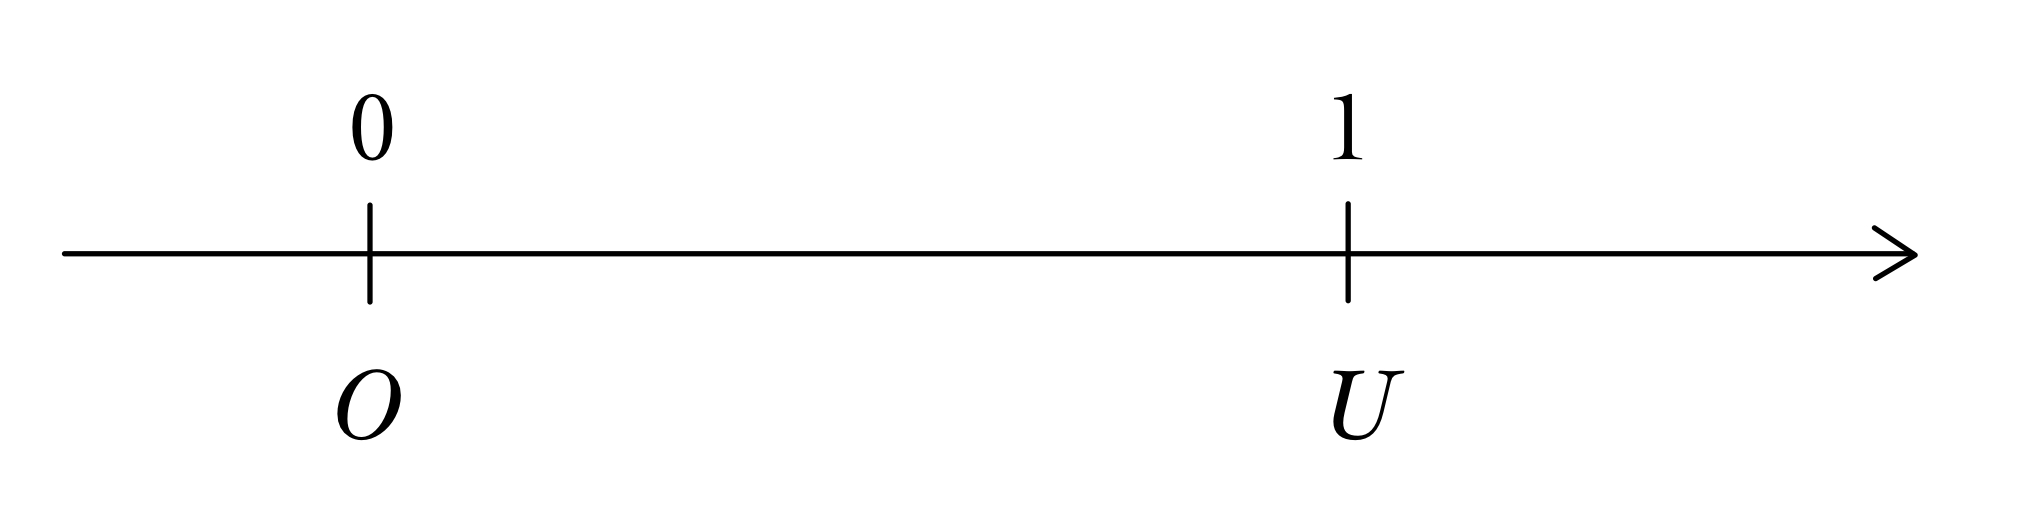
\includegraphics[width=0.5\textwidth]{number_line.PNG}\figtag{1.1.1}
\end{center}

In this manner we establish a one-to-one correspondence between the points of a line and the numbers of the real number system. Figure 1.2.2 shows some real numbers represented as points on the number line. Positive numbers appear to the right of $0$, negative numbers to the left of $0$.

\begin{center}
    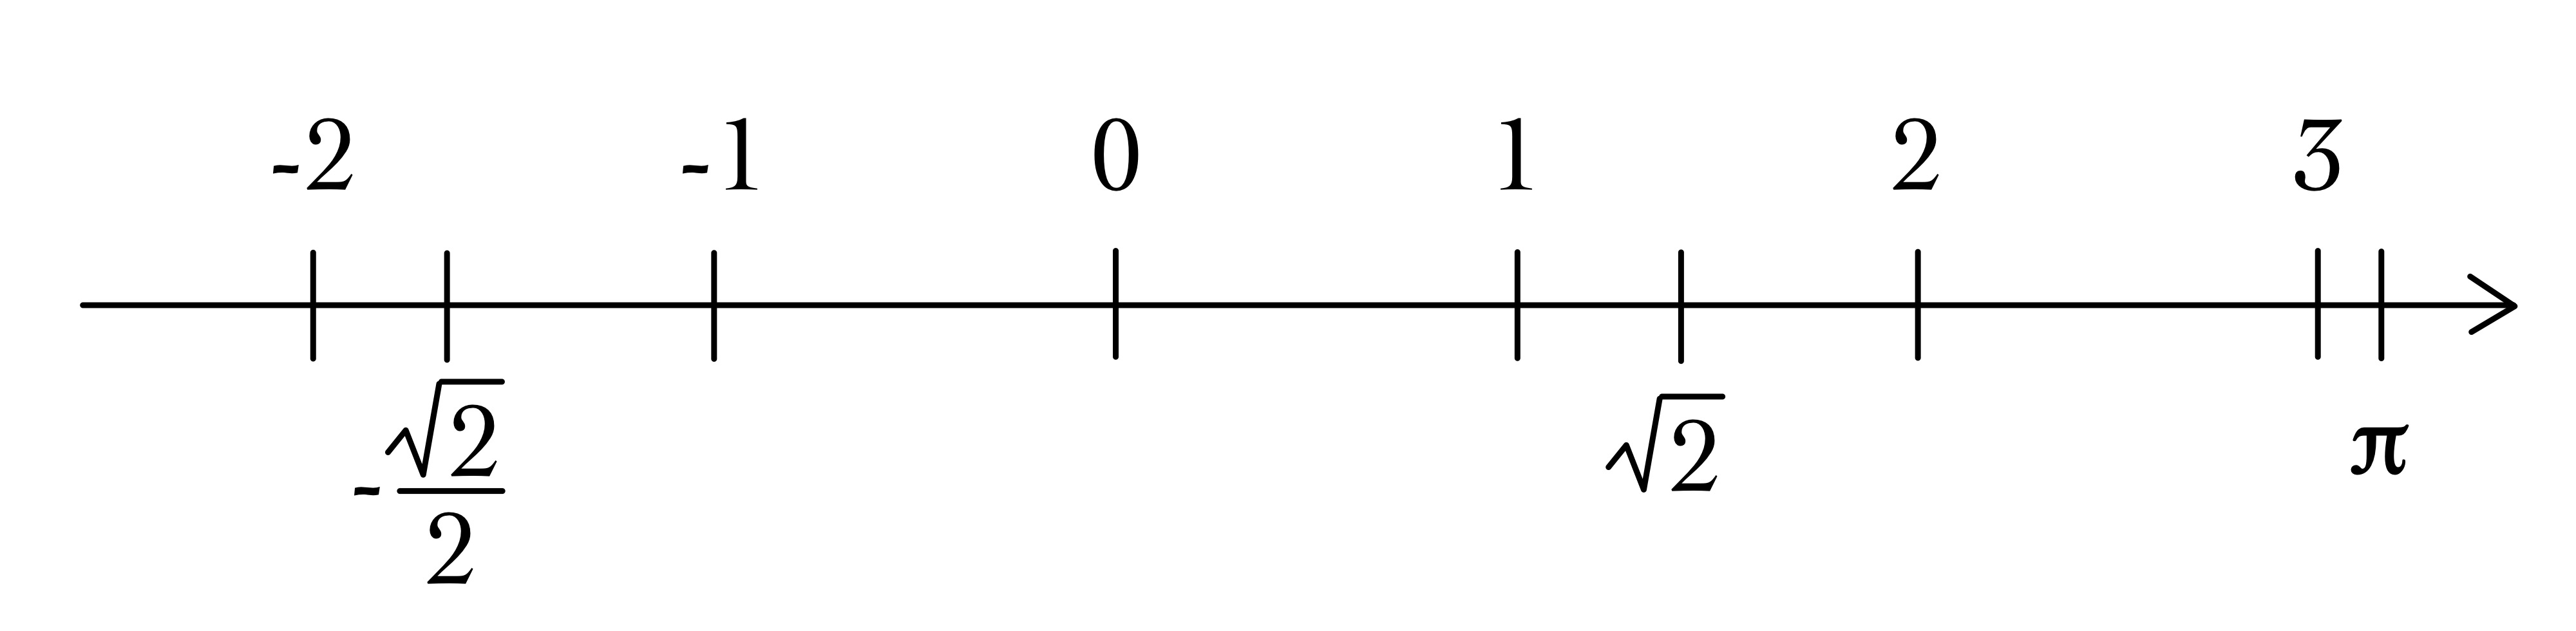
\includegraphics[width=0.65\textwidth]{number_line_example.JPG}\figtag{1.1.2}
\end{center}

\subsection*{Absolute Value}

Let $a\in\bbR$. The symbol $|a|$ is called ``the absolute value of $a$,'' and is defined by \vspace*{0.5em} \begin{equation*}
    |a|=\left\{\begin{array}{rl}a,&\quad\text{if $a\geq0$,}\\-a&\quad\text{if $a<0$.}\end{array}\right.\\[0.5em]
\end{equation*} The geometric meaning of $|a|$ is the distance between $a$ and $0$. Moreover, $|a-b|$ is the distance between $a$ and $b$.

We have some properties regarding the absolute values. 

\begin{theorem}
    Let $a, b\in\bbR$. The following statements hold.
    \begin{enumerate}
        \item $|a|=0$ if and only if $a=0$.
        \item $|-a|=|a|$.
        \item $|ab|=|a||b|$.
        \item (\textit{Triangle Inequality}) $|a+b|\leq|a|+|b|$.
        \item (\textit{Reverse Triangle Inequality}) $||a|-|b||\leq|a-b|$.
        \item $|a^2|=|a|^2=a^2$.
    \end{enumerate}
\end{theorem}

\subsection*{Interval}

Accurately, intervals are connected subsets in the real number system. We use a pair of parentheses with a comma $(\cdot, \cdot)$ to indicate open intervals and use a pair of brackets with a comma $[\cdot, \cdot]$ to indicate closed intervals.

Suppose $a<b$. The open interval $(a, b)$ is the set of all numbers between $a$ and $b$: $$(a, b)=\{x\in\bbR\mid a<x<b\}.$$
\begin{center}
    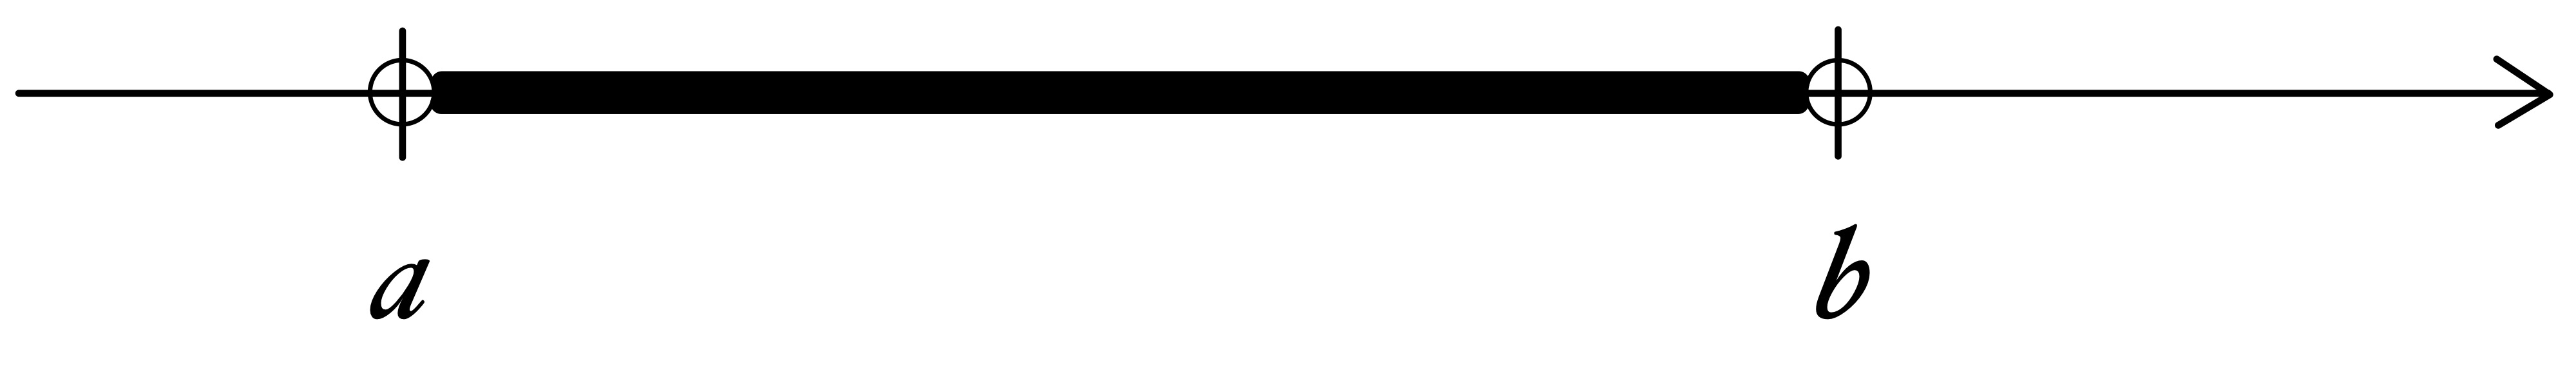
\includegraphics[width=0.45\textwidth]{interval_oo.JPG}
\end{center}
The closed interval $[a, b]$ is the open interval $(a, b)$ with endpoints $a$ and $b$: $$[a, b]=\{x\in\bbR\mid a\leq x\leq b\}.$$
\begin{center}
    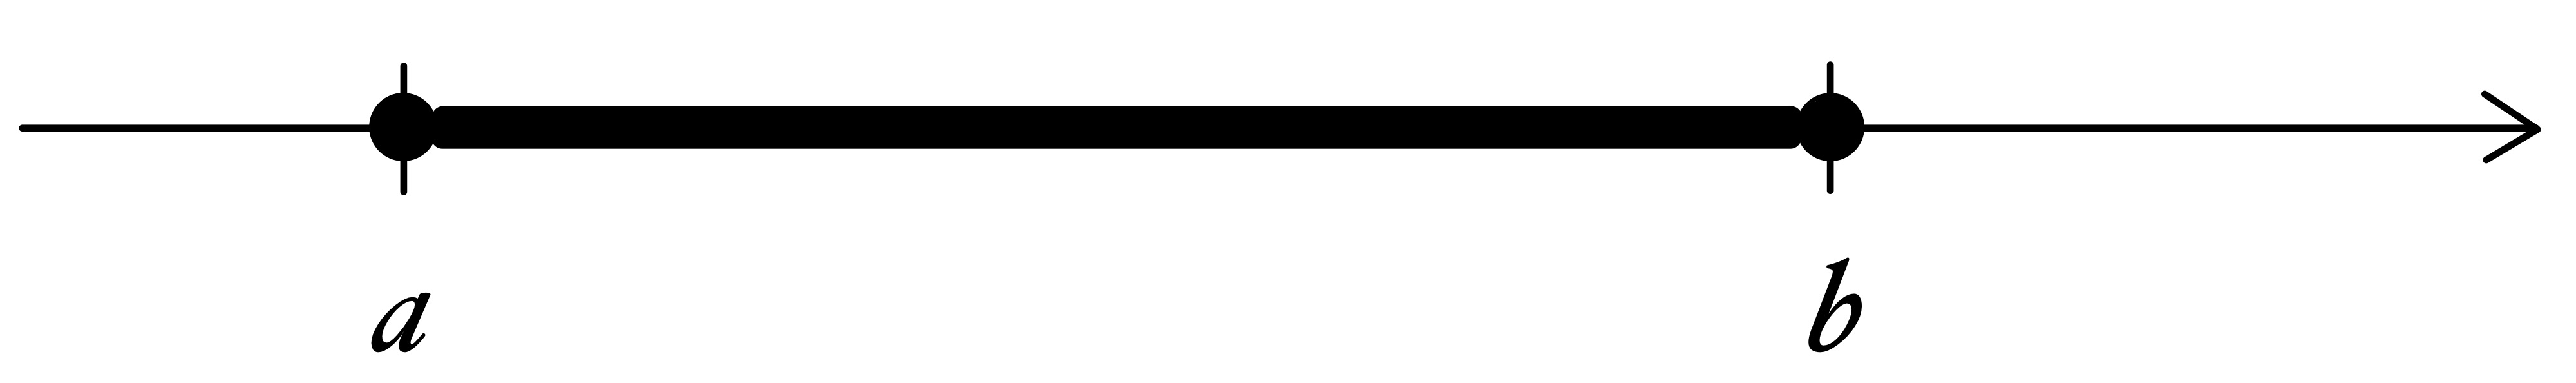
\includegraphics[width=0.45\textwidth]{interval_cc.JPG}
\end{center} We have seven more types of intervals: \begin{align*}
    (a, b]&=\{x\in\bbR\mid a<x\leq b\},\\
    [a, b)&=\{x\in\bbR\mid a\leq x<b\},\\
    (a, \infty)&=\{x\in\bbR\mid x>a\},\\
    [a, \infty)&=\{x\in\bbR\mid x\geq a\},\\
    (-\infty, b)&=\{x\in\bbR\mid x<b\},\\
    (-\infty, b]&=\{x\in\bbR\mid x\leq b\},\\
    (-\infty, \infty)&=\bbR.
\end{align*}

Interval notation is easy to remember: we use a square bracket to include an endpoint and a parenthesis to exclude it. On a number line, inclusion is indicated by a solid dot, exclusion by an open dot. The symbols $\infty$ and $-\infty$, read “infinity” and “negative infinity” (or “minus infinity”), do not represent real numbers. In the intervals listed above, the symbol $\infty$ is used to indicate that the interval extends indefinitely in the positive direction; the symbol $-\infty$ is used to indicate that the interval extends indefinitely in the negative direction.

\subsection*{Basic Algebra}

We use a small number on the top-right of another number to indicate the ``power'', which essentially means the number of multiplication.
\begin{notation}
    Let $r\in\bbR$ and $p\in\bbN\cup\{0\}$. If $p\ne0$, then the number $r^p$ is read ``$r$ to the power $p$'' and is with value $\overbrace{r\times r\times \cdots\times r}^{\text{$p$ times}}$. This explanation only works when the power is a positive integer. If $p=0$ and $r\ne0$, we define $r^0=1$. The number $r$ is called the ``base,'' $p$ is called the ``exponent,'' and $r^p$ is called the ``power.''
\end{notation}

\begin{example}
    By the texts above, we have 
    \begin{enumerate}
        \item $(-2)^2=4$,
        \item $5^4=625$,
        \item $(-1)^5=-1$.
    \end{enumerate}
\end{example}

\begin{notation}
    Let $a>0$ and $p>0$. The number $a^{1/p}$ is called the $p$-th root of $a$ and is the number $b$ such that $b^q=a$; it can also be written as $\sqrt[q]{a}$. If $p=2$, we just write $\sqrt{a}$. The number $a^{-p}$ is the reciprocal of $a^p$.
\end{notation}

We have some special formulas for products and quotients of powers.

\begin{theorem}[Laws of Exponents]
    Let $a>0$ and $p, q\in\mathbb R$. The following hold.
    \begin{enumerate}
        \item $a^{p+q}=a^p+a^q$.
        \item $a^{p-q}=\dfrac{a^p}{a^q}$.
        \item $(a^p)^q=a^{pq}$.
    \end{enumerate}
\end{theorem}

\begin{example}
    Show that $$a^0=1$$ with the laws of exponents given $a>0$.
\end{example}
\textbf{Proof}. Using $$a^{p-q}=\dfrac{a^p}{a^q},$$ we have 
\begin{align*}
    a^0&=a^{1-1}\\
    &=\dfrac{a^1}{a^1}\\
    &=1,
\end{align*}
which coincides the definition. \qed

Furthermore, we can combine products with summations, factorizing an expression, so that we can find a root more easily.

\begin{theorem}[Factorization]
    Let $a, b\in\bbR$. The following hold.
    \begin{enumerate}
        \item $(a+b)^2=a^2+2ab+b^2$.
        \item $(a-b)^2=a^2-2ab+b^2$.
        \item $(a+b)^3=a^3+3a^2b+3ab^2+b^3$.
        \item $(a-b)^3=a^3-3a^2b+3ab^2-b^3$.
        \item $a^2-b^2=(a-b)(a+b)$.
        \item $a^3-b^3=(a-b)(a^2+ab+b^2)$.
        \item $a^n-b^n=(a-b)(a^{n-1}+a^{n-2}b+\cdots+ab^{n-2}+b^{n-1})$.
    \end{enumerate}
\end{theorem}

\begin{example}
    Evaluate the following numbers.
    \begin{enumerate}
        \item $255^2-245^2$.
        \item $25+2950+295^2$.
    \end{enumerate}
\end{example}
\textbf{Solution}. For the first number, we use $$a^2-b^2=(a-b)(a+b)$$ with $a=255$ and $b=245$. Hence, $255^2-245^2=10\cdot500=5000$. For the second number, we use $$(a+b)^2=a^2+2ab+b^2,$$ reversely, with $a=5$ and $b=295$. Hence, $25+2950+295^2=(300)^2=90000$. \qed

\begin{example}
    Factorize the following expressions.
    \begin{enumerate}
        \item $x^2-4x+3$.
        \item $x^2+2x-3$.
        \item $x^2+6x+8$.
    \end{enumerate}
\end{example}
\textbf{Solution}. For the first expression, obeserve that $-4=(-3)+(-1)$ and $(-3)\cdot(-1)=+3$. Hence, $$x^2-4x+3=(x-3)(x-1).$$ For the second expression, obeserve that $2=3+(-1)$ and $3\cdot(-1)=-3$. Hence, $$x^2+2x-3=(x+3)(x-1).$$ For the last expression, observe that $6=2+4$ and $2\cdot4=8$. Hence, $$x^2+6x+8=(x+2)(x+4).$$ \qed

Factorization is crucial for solving inequalities and finding roots.

\begin{theorem}[Quadratic Formula]
    Let $a\ne0$, $b, c\in\bbR$. The roots of the equation $$ax^2+bx+c=0$$ are $$x=\dfrac{-b\pm\sqrt{b^2-4ac}}{2a}.$$ The expression $b^2-4ac$ inside the square root is called the ``discriminant'' and is denoted by $D$. If $D>0$, the equation has two distinct real roots. If $D=0$, the equation has one real root. If $D<0$, the equation has two complex roots.
\end{theorem}

\begin{example}
    Solve the equation $$2x^2+3x-2=0.$$
\end{example}
\textbf{Solution}. Using the quadratic formula, $$x=\dfrac{-3\pm\sqrt{3^2+4\cdot2\cdot(-2)}}{2\cdot 2}.$$ Hence, $x=\dfrac{1}{2}$ or $x=-2$. \qed

\subsection*{Exercise}
\begin{enumerate}[label=\arabic*.]
    \item Answer the following questions.
    \begin{enumerate}
        \item We have four people, Anne, Bell, Christine, and Derek, comparing their heights. Suppose Christine is shorter than Anne, Bell is taller than Derek, and Christine is taller than Bell. Arrange them with their heights.
        \item Suppose $a+2=b+20=c-4$. What is the biggest number? What is the smallest number?
    \end{enumerate}
    \item Determine true or false for each of the following statements.
    \begin{enumerate}
        \item $1$ is the smallest positive integer.
        \item $-1$ is the smallest negative integer.
        \item $0$ is an integer.
        \item $1$ is the smallest positive integer.
    \end{enumerate}
    \item Answer the following questions.
    \begin{enumerate}
        \item How many points are there is with unit length $4$ to the origin?
        \item Evaluate the following expressions.
        \begin{multicols}{4}
            \begin{enumerate}[label=\alph*.]
                \item $|-5|-|8|$.
                \item $|-3-7|$.
                \item $|5-\sqrt{5}|$.
                \item $|2-\pi|$.
            \end{enumerate}
        \end{multicols}
        \item Does the equation $\sqrt{a^2}=a$ hold for all $a\in\bbR$?
        \item Suppose moving $6$ meters to the right of the origin can be denoted as $+2$. How can moving $15$ meters to the left of the origin be denoted?
        \item There are three points $A$, $B$, and $C$ on the number line, with coordinate $1$, $6$, and $8$, respectively. Suppose one set the origin to $B$ without changing the unit length. What is the coordinate of $A$? What is the coordinate of $C$?
        \item If $a-b=18$ and $|a|=|b|$, what are $a$ and $b$?
        \item If $a$ and $b$ are with different signs, i.e., $ab<0$, and $|a|=|b|$, what is the value of $a+b$?
        \item Suppose $a$ and $b$ are all negative. If $|a|>|b|$, what is the order between $a$ and $b$?
    \end{enumerate}
    \item Answer the following questions.
    \begin{enumerate}
        \item If $3|a+2|+2|b-7|=0$, what are $a$ and $b$?
        \item If $|4-a|=1$, what is $a$?
        \item If $a>0$, what is $|a|$?
        \item If $a<0$, what is $|a|$?
        \item How many integers $a$ are there satisfying $4<|a|<7$?
        \item How many integers $c$ are there satisfying $|c|\leq 4$?
        \item If $|a-2|=2$, what is $a$?
        \item If $|c+2|=8$, what is $c$?
    \end{enumerate}
    \item Answer the following questions.
    \begin{enumerate}
        \item What is $[0, 2]\cap(2, 4)$?
        \item What is $[0, 1]\setminus(0, \infty)$?
        \item What is the interval $I$ such that only elements $x$ in $I$ suffice $|x|\leq 3$?
        \item What is the interval $J$ such that only elements $x$ in $J$ suffice $x^2<16$?
    \end{enumerate}
    \item Answer the following questions.
    \begin{enumerate}
        \item If $25^{3m}=3$ and $5^{7n}=\dfrac{1}{3}$, what is the value of $(6m+7n-2)^5$?
        \item If $8^{2a}=4$, what is the value of $8^{6a}$?
        \item If $x^{2a}=3$, what is the value of $\dfrac{x^{3a}-x^{-a}}{x^{3a}+x^{-a}}$?
        \item If $a\cdot567^3=10^3$ and $\dfrac{a}{10^3}=b$, what is the value of $a\cdot b$?
    \end{enumerate}
    \item Factorize the following expressions.
    \begin{multicols}{2}
        \begin{enumerate}
            \item $x(b-c)-y(c-b)$.
            \item $(x-a)(x-3)+(3-x)(x-b)$.
            \item $(x^2+6x)^2-9^2$.
            \item $(x^2+3x)^2-(x+4)^2$.
            \item $x^2+4x+4-y^2$.
            \item $9x^2+6x+1$.
        \end{enumerate}
    \end{multicols}
    \item Find the real roots of the equation.
    \begin{multicols}{2}
        \begin{enumerate}
            \item $x^2-x-2=0$.
            \item $x^2-9=0$.
            \item $x^2-6x+9=0$.
            \item $x^2+8x+16=0$.
            \item $x^2-2x+5=0$.
            \item $(x-3)^2-16=0$.
        \end{enumerate}
    \end{multicols}
\end{enumerate}

\section{Inequalities}

Inequalities can be similarly solved like one solving an equation, adding the same number to both sides or by multiplying both sides by the same positive number. The relation will be reversed when multiplied both sides by the same negative number.

\begin{example}
    Solve the inequality $$-4(3-x)\leq 12.$$
\end{example}
\textbf{Solution}. Multiplying both sides by $\dfrac{1}{4}$, we have $$x-3\leq 3.$$ Adding $3$ to both sides, we have $$x\leq 6.$$ Hence, the solution set is the interval $(-\infty, 6]$. \qed

\begin{example}
    Solve the inequality $$x^2-4x+3>0.$$
\end{example}
\textbf{Solution}. Factorizing the expression on the left, we have $$(x-3)(x-1)>0.$$ The inequality only holds when the expression $(x-3)$ and the expression $(x-1)$ are with the same sign. That is, the inquality only holds when \begin{enumerate}
    \item $x-3>0$ and $x-1>0$, or
    \item $x-3<0$ and $x-1<0$.
\end{enumerate}
For the first scenario, $(3, \infty)$ is the set of solutions. For the second scenario, $(-\infty, 1)$ is the set of solutions. Hence, the set of solutions for the inequality is $(-\infty, 1)\cup(3, \infty)$. \qed

\begin{example}
    Solve the inequality $$|x+2|<3.$$
\end{example}
\textbf{Solution}. Using the geometric meaning of the absolute value, the set of solutions is the set containing points with distance less than $3$ to point $-2$. Hence, the set of solutions is $(-5, 1)$. \qed\\
\textbf{Alternative Solution}. We can write $|x+2|<3$ as $-3<x+2<3.$ Adding $-2$ to each expression of the inequalities, we have $-5<x<1.$\qed

\begin{theorem}[Triangle inquality]
    Let $a, b\in\bbR$. The inequality $$|a+b|\leq |a|+|b|$$ must hold.
\end{theorem}
\textbf{Proof}. We have the natural equality $2ab\leq2|ab|$. Adding $a^2+b^2$ to both sides, we have $$a^2+2ab+b^2\leq |a|^2+2|a||b|+|b|^2.$$ Since both sides are non-negative, taking square roots yeilds $|a+b|\leq |a|+|b|.$ \qed

\subsection*{Exercise}
\begin{enumerate}[label=\arabic*.]
    \item Solve the following inqualities. Afterwards, express the solution set as an interval or as the union of intervals and mark the solution set on a number line.
    \begin{multicols}{3}
        \begin{enumerate}
            \item $2+3x<5$.
            \item $16x+64\leq16$.
            \item $7x(x-4)^2<0$.
            \item $|x|<2$.
            \item $0<|x|<1$.
            \item $|3x+1|>5$.
        \end{enumerate}
    \end{multicols}
    \item Each of the following sets is the solution of an inequality of the form $|x-c|<\delta$. Find $c$ and $\delta$.
    \begin{multicols}{3}
        \begin{enumerate}
            \item $(-3, 3)$.
            \item $(-3, 7)$.
            \item $(-7, 3)$
            \item $(0, 4)$.
            \item $(0, b)$.
            \item $(a, b)$.
        \end{enumerate}
    \end{multicols}
    \item Given that $x>1$, arrange the following in order: $$1, x, \sqrt{x}, \dfrac{1}{x}, \dfrac{1}{\sqrt{x}}.$$
    \item Given that $0<x<1$, arrange the following in order: $$1, x, \sqrt{x}, \dfrac{1}{x}, \dfrac{1}{\sqrt{x}}.$$
\end{enumerate}

\section{Functions}

Functions can be imagined as a black box. You throw a parameter $x$ into the black box $f$, and then you obtain the result $f(x)$. Mathematically speaking, a function is a correspondence between two sets, domain and range. For example, a teacher is marking exams for students. There are twenty questions in total. A student gets five points with a correct answer to a question. In this case, the score is a function of the number of correct answers. In mathematical language, we say the score is $f_{\text{score}}(x)=5x$, where $x$ is the number of correct answers. Since the number of correct answers can only be positive integers among $0$ and $20$, we say the domain (the set where the function is valid) is $\{0, 1, 2, \dots, 19, 20\}$. The range, the set with all positive outcomes for the function, is $\{0, 5, 10, \dots, 95, 100\}$ in this case.

To be more specific, we use a colon ``$:$'' and an arrow ``$\to$'' to indicate the function and its domain and codomain (a set that contains the range). One generally indicates codomain since one does not know exactly the range is. For example, I can write $f_{\text{score}}:\{0, 1, 2, \dots, 19, 20\}\to\bbN$, which indicates that the domain of the function $f_{\text{score}}$ is $\{0, 1, 2, \dots, 19, 20\}$, and all the outputs will be in $\bbN$.

Take another familiar example, the square function $f_{\text{square}}$. The square function outputs the square of an input. Since you can square any real numbers, we write $f_{\text{square}}:\bbR\to\bbR$ with $f(x)=x^2$ for all $x\in\bbR$, or more specificly, $f_{\text{square}}:\bbR\to\bbR_{\geq0}$ with $f(x)=x^2$ for all $x\in\bbR$. One can use the arrow with a small stroke on the left ``$\mapsto$'' to indicate the way of mapping. For example, $x\mapsto x^2$ is the square function. We are familiar with the absolute value. In fact, the absolute value is a function with domain $\bbR$ and range $[0, \infty)$.

Usually, we call the input $x$ the independent variable (or argument), and we call the output $y$ the dependent variable, since $y$ varies on $x$.

\begin{definition}[Injective, Surjective, and Bijective]
    A function $f:X\to Y$ is \underline{injective} if $x_1\ne x_2\in X$ implies $f(x_1)\ne f(x_2)$. A function $g:X\to Y$ is \underline{surjective} if there exists a $x\in X$ such that $f(x)=y$ for all $y\in Y$. A function is bijective if it is surjective and injective.
\end{definition}

\begin{definition}[Graph]
    Let $f:X\to Y$ be a function. The \underline{graph} of $f$ is the set $$\{(x, y)\mid x\in X\text{ and }y=f(x)\}.$$
\end{definition}

\subsection*{Symmetry}

\begin{definition}[Even and Odd]
    A function $f:X\to Y$ is said to be \underline{even} if $f(x)=f(-x)$ for all $x\in X$. A function $g:X\to Y$ is said to be \underline{odd} if $f(x)=g(-x)$ for all $x\in X$.
\end{definition}

Functions in both genres are all called ``symmetric'' since an even function is symmetric from the $y$-axis, and an odd function is symmetric from the origin.

\begin{example}
    Determine whether the following functions are even, odd, or neither.
    \begin{enumerate}
        \item $f_1(x)=x$.
        \item $f_2(x)=x+1$.
        \item $f_3(x)=|x|$.
        \item $f_4(x)=x^2$.
        \item $f_5(x)=x^3$.
        \item $f_6(x)=2^x+2^{-x}$.
    \end{enumerate}
\end{example}
\textbf{Solution}. The function $f_1$ is odd since $f_1(x)=x=-f_1(x)=-(-x)$. The function $f_2$ is neither even nor odd. The function $f_3$ is even since $|x|=|-x|$. The function $f_4$ is also even. The function $f_5$ is odd. The function $f_6$ is even since $f_6(x)=2^x+2^{-x}=f_6(-x)=2^{-x}+2^x$. \qed

\subsection*{Exercise}

\begin{enumerate}[label=\arabic*.]
    \item Calculate $f(0), f(1), f(-1)$ with the following functions.
    \begin{multicols}{3}
        \begin{enumerate}
            \item $f(x)=|x|$.
            \item $f(x)=x^3$.
            \item $f(x)=2x^2-3x+2$.
            \item $f(x)=\dfrac{2x-1}{x^2+4}$.
            \item $f(x)=\sqrt{x^2+2x+5}$.
            \item $f(x)=|x+3|-5x$.
        \end{enumerate}
    \end{multicols}
    \item Calculate $f(a), f(-a), f(a+h), \dfrac{f(a+h)-f(a)}{h}$ with the following functions.
    \begin{multicols}{2}
        \begin{enumerate}
            \item $f(x)=3x+2$.
            \item $f(x)=x^2-2x$.
            \item $f(x)=2x^2-3x$.
            \item $f(x)=\dfrac{1}{x-2}$.
        \end{enumerate}
    \end{multicols}
    \item Give the domain and range of the function.
    \begin{multicols}{2}
        \begin{enumerate}
            \item $f(x)=|x|$.
            \item $f(x)=\dfrac{1}{x^2}$.
            \item $f(x)=\sqrt{x-3}$.
            \item $f(x)=\dfrac{1}{\sqrt{2-x}}$.
        \end{enumerate}
    \end{multicols}
    \item Give the domain and range of the function and sketch the graph of the function.
    \begin{multicols}{2}
        \begin{enumerate}
            \item $f(x)=1$.
            \item $f(x)=-1$.
            \item $f(x)=x$
            \item $f(x)=2x$.
            \item $f(x)=2x+1$.
            \item $f(x)=2x-1$.
            \item $f(x)=|x|$.
            \item $f(x)=|x-1|$.
            \item $f(x)=|x+1|$.
            \item $f(x)=\left\{\begin{array}{rl}
                -1,\quad&\text{if $x<0$,}\\1,\quad&\text{if $x>0$}.
            \end{array}\right.$
        \end{enumerate}
    \end{multicols}
    \item Determin whether the following functions are even, odd, or neither.
    \begin{multicols}{2}
        \begin{enumerate}
            \item $f(x)=x^2+1$.
            \item $f(x)=\dfrac{x^2}{1-|x|}$.
            \item $f(x)=x+\dfrac{1}{x}$.
            \item $f(x)=\sqrt[5]{x-x^3}$.
        \end{enumerate}
    \end{multicols}
\end{enumerate}

\section{Elementary Functions}

The functions that figure most prominently in single-variable calculus are the polynomial functions, the rational functions, the trigonometric functions, the exponential functions, and the logarithmic functions. These functions are generally known as the elementary functions.

\subsection*{Polynomial Functions}

\begin{definition}[Polynomial]
    Let $n\in\bbN\cup\{0\}$. An expression of the form $$a_nx^n+a_{n-1}x^{n-1}+\cdots+a_1x+a_0$$ with $a_i\in\bbR$, $i=0, 1, \dots, n$, is a \underline{polynomial}. This is called a real polynomial of degree $n$.
\end{definition}

\begin{example}
    The following are polynomials.
    \begin{enumerate}
        \item $x^2+x+1$.
        \item $-\pi x^4-7$.
        \item $x^{256}$.
        \item $0$.
    \end{enumerate}
\end{example}

\begin{example}
    The following are \textbf{NOT} polynomials.
    \begin{enumerate}
        \item $x+1+\dfrac{1}{x}$.
        \item $|x|+5$.
        \item $\sqrt{2x}-7$.
    \end{enumerate}
\end{example}

\begin{definition}[Polynomial Function]
    A \underline{polynomial function} $P$ is a function with output a polynomial, i.e., $P(x)=a_nx^n+a_{n-1}x^{n-1}+\cdots+a_1x+a_0$.
\end{definition}

\begin{theorem}[Fundamental Theorem of Algebra]
    Every single-variable real polynomial of degree $n$ has exactly $n$ complex roots counted with multiplicity.
\end{theorem}

\subsection*{Rational Functions}

\begin{definition}[Rational Function]
    A \underline{rational function} is the quotient of two polynomial functions, i.e., $R(x)=\dfrac{P_1(x)}{P_2(x)}$.
\end{definition}

A rational function will have a vertical asymptote at $a$ such that $P_2(a)=0$. For example, the function $f(x)=\dfrac{1}{x}$ has a vertical asymptote at $0$. See Figure 1.4.1. We will talk about this in Chapter 4.

\begin{center}
    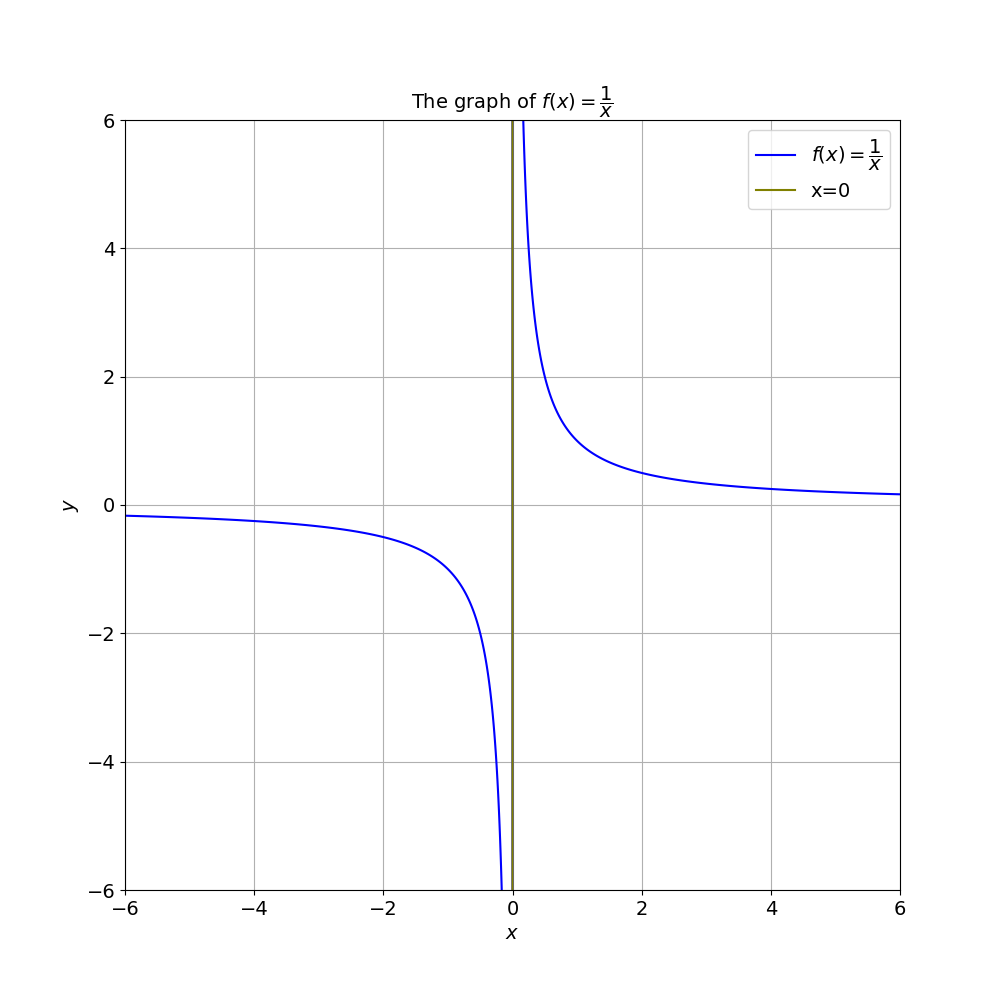
\includegraphics[width=0.5\textwidth]{reciprocal_of_x.png}\figtag{1.4.1}
\end{center}

\begin{example}
    Find vertical asymptotes of the following functions.
    \begin{enumerate}
        \item $f_1(x)=\dfrac{1}{x^2+4x+4}$.
        \item $f_2(x)=\dfrac{1}{x^2-1}$.
    \end{enumerate}
\end{example}
\textbf{Solution}. For function $f_1$, since $x^2+4x+4=(x+2)^2$, the vertical asymptote is $x=-2$. For function $f_2$, since $x^2-1=(x+1)(x-1)$, the vertical asymptotes are $x=1$ and $x=-1$. \qed

\subsection*{Trigonometric Functions}

Trigonometric functions are originally the ratio between sides of a right triangle. For example, if I have a triangle with lengths $a, b, c$ and an angle $\theta$.

\begin{center}
    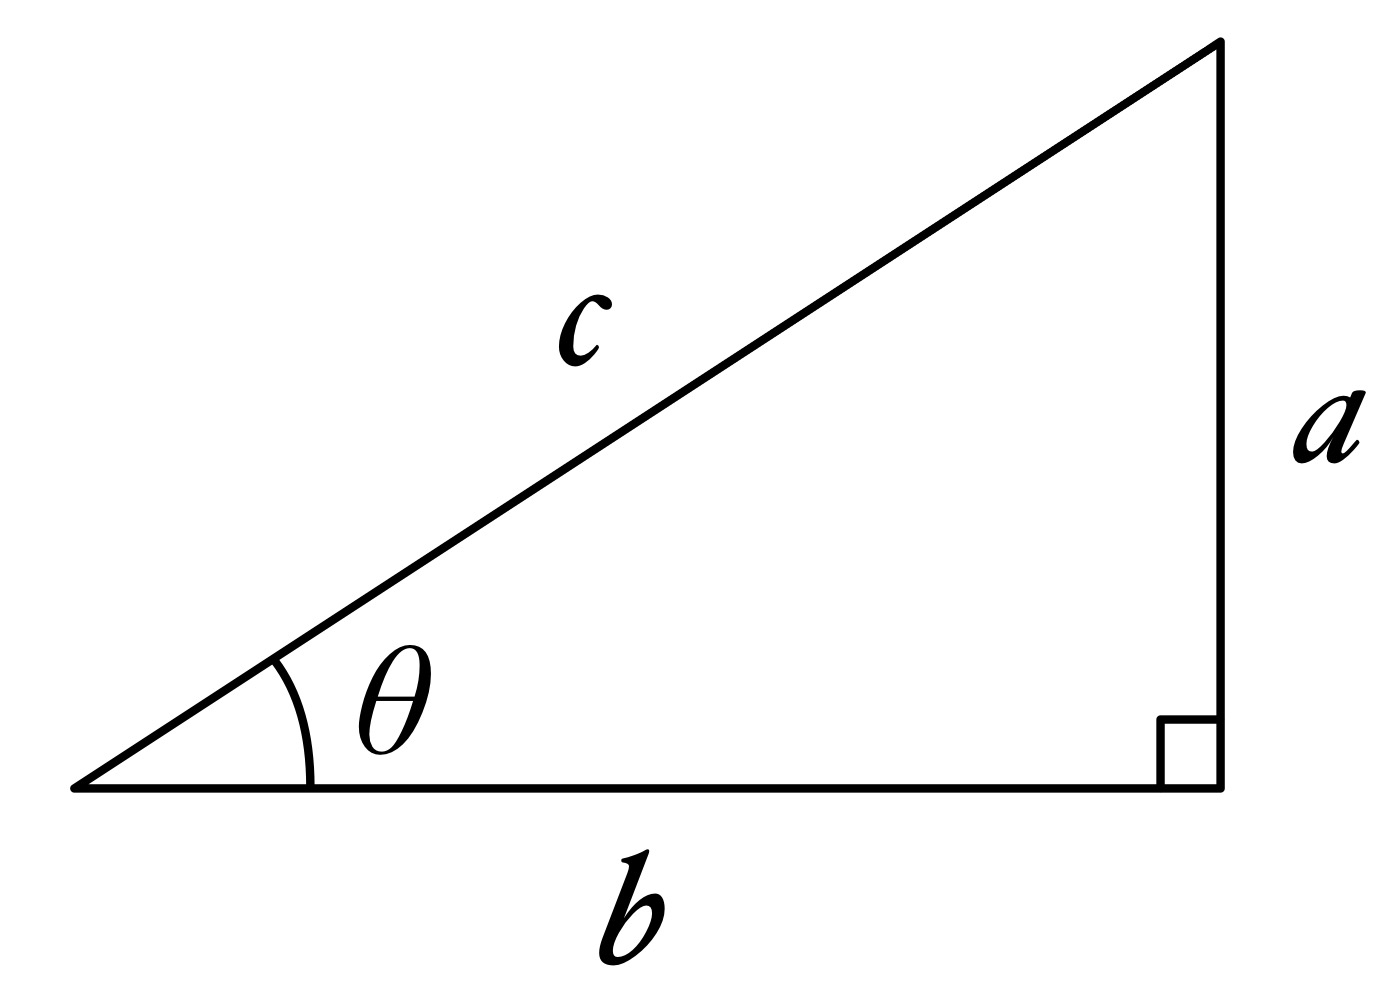
\includegraphics[width=0.2\textwidth]{triangle.JPG}\figtag{1.4.2}
\end{center}

The ratio $\dfrac{a}{c}$ of the length of the hypotenuse $c$ to the length of the opposite leg $a$ is called $\sin\theta$. The ratio $\dfrac{b}{c}$ of the length of the hypotenuse $c$ to the length of the adjecent leg $b$ is called $\cos\theta$. The ratio $\dfrac{\sin\theta}{\cos\theta}$ is called $\tan\theta$, is also the ratio of the length of the adjecent leg $b$ to the length of the opposite leg $a$.

\subsubsection*{Radian Measure}

Degree measure, traditionally used to measure angles, has a serious
drawback. It is artificial; there is no intrinsic connection between a degree and the geometry of a rotation. Why choose $360^\circ$ for one complete revolution? Why not $100^\circ$ or $400^\circ$? There is another way of measuring angles that is more natural and lends itself better to the methods of calculus: measuring angles in radians.

We first introduce $\pi$, the ratio of the length of a half circumference of a circle to the length diameter of the circle. Since a hald circumference is just a half circle, we say that $\pi\ \text{rad}$ is $180^\circ$. Hence, $2\pi\ \text{rad}$ is $360^\circ$. The following table gives some common angles (rotations) measured both in degrees and in radians.

\begin{center}
    \begin{tabular}{|cccccccccccc|}
        \hline
        degrees & $0^\circ$ & $30^\circ$ & $45^\circ$ & $60^\circ$ & $90^\circ$ & $120^\circ$ & $135^\circ$ & $150^\circ$ & $180^\circ$ & $270^\circ$ & $360^\circ$\\
        \hline
        radians & $0$ & $\dfrac{1}{6}\pi$ & $\dfrac{1}{4}\pi$ & $\dfrac{1}{3}\pi$ & $\dfrac{1}{2}\pi$ & $\dfrac{2}{3}\pi$ & $\dfrac{3}{4}\pi$ & $\dfrac{5}{6}\pi$ & $\pi$ & $\dfrac{3}{2}\pi$ & $2\pi$\\[0.2em]
        \hline
    \end{tabular}
\end{center}

\subsubsection*{Sine and Cosine}

Let $\theta$ be any real number. The rotation $\theta$ takes the point $A$ with coordinates $(1, 0)$ to some point $P$, also on the unit circle. The coordinates of $P$ are completely determined by $\theta$ and have names related to $\theta$. The second coordinate of $P$ is $\sin\theta$, and the first coordinate of $P$ is $\cos\theta$. Figure 1.4.3 illustrates the idea. To simplify the diagram, we have taken $\theta$ from $0$ to $2\pi$.

For each real $\theta$, the rotation $\theta$ and the rotation $\theta+2\pi$ take the point $A$ to exactly the same point $P$. If follows that for each $\theta$, $$\sin(\theta+2\pi)=\sin\theta\qquad\text{and}\qquad\cos(\theta+2\pi)=\cos\theta.$$

\begin{center}
    \begin{minipage}{0.48\textwidth}
        \begin{center}
            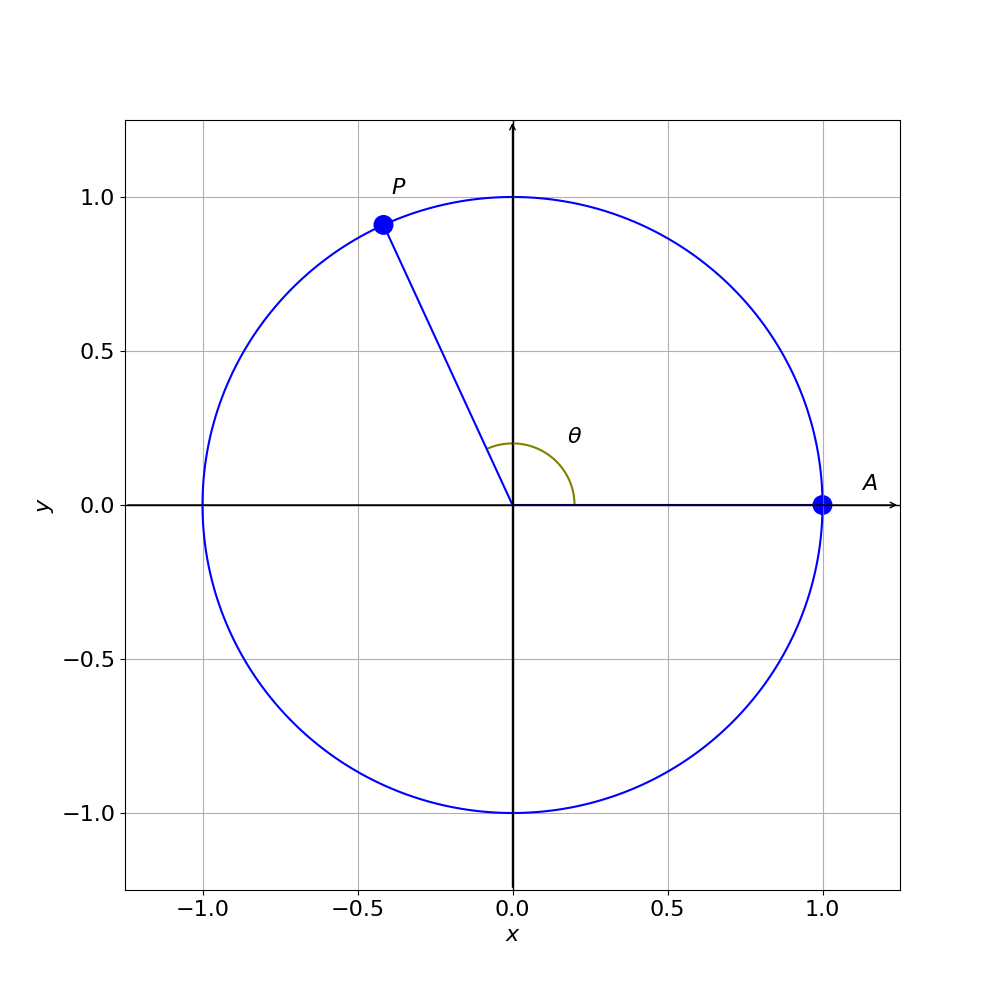
\includegraphics[width=0.85\textwidth]{unit_circle_1.png}\figtag{1.4.3}
        \end{center}
    \end{minipage}
    \begin{minipage}{0.48\textwidth}
        \begin{center}
            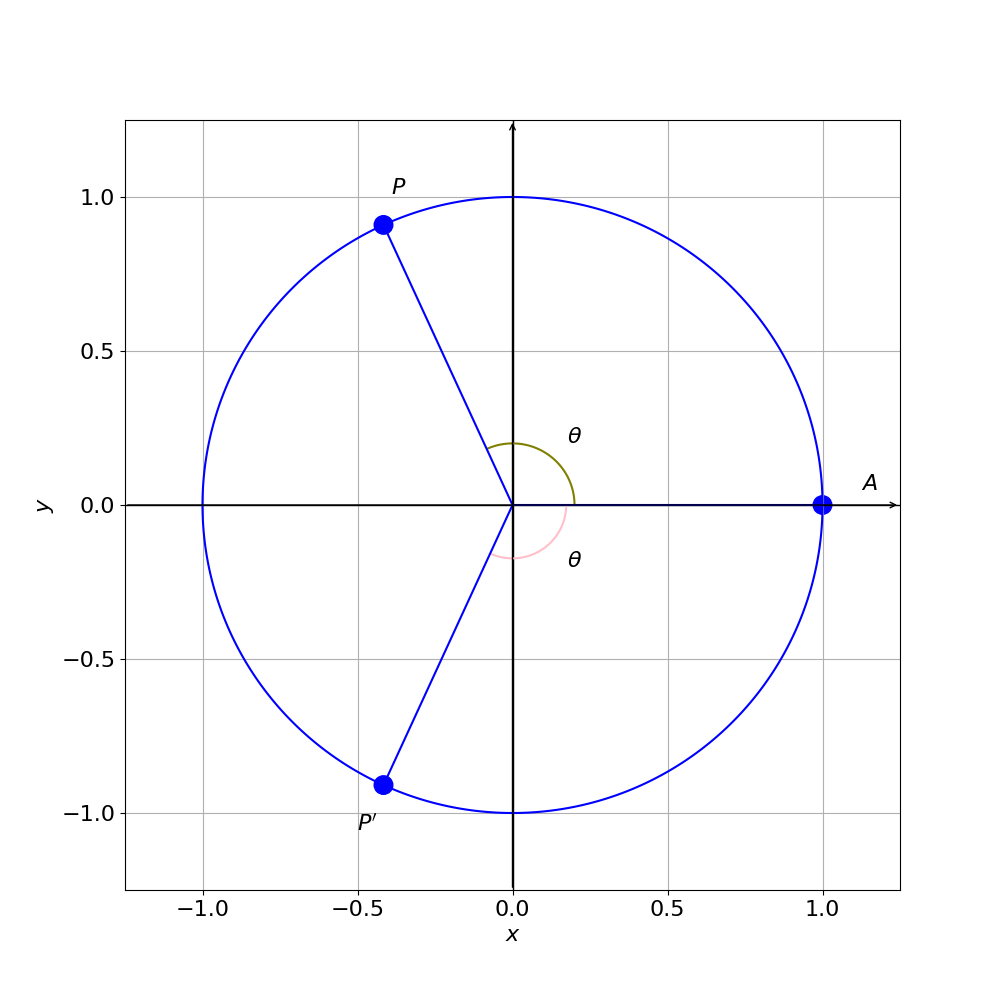
\includegraphics[width=0.85\textwidth]{unit_circle_2.png}\figtag{1.4.4}
        \end{center}
    \end{minipage}
\end{center}

\vspace*{1.5em}

A rotation of $\pi\ \text{rad}$ takes each point to the point antipodal to it: $(x, y)\mapsto(-x, -y)$. Thus, $$\sin(\theta+\pi)=-\sin\theta\qquad\text{and}\qquad\cos(\theta+\pi)=-\cos\theta.$$

In Figure 1.4.4, we consider two rotations, a positive rotation $\theta$ and its negative counterpart $-\theta$, from point $A$ respectively to point $P$ and to point $P'$. From the figure, you can see that $$\sin(-\theta)=-\sin\theta\qquad\text{and}\qquad\cos(-\theta)=\cos\theta.$$

\subsubsection*{Tangent, Cotangent, Secant, Cosecant}

We have four more trigonometric functions: the tangent, the cotangent, the secant, the cosecant. These are obtained as follows: $$\tan\theta=\dfrac{\sin\theta}{\cos\theta},\qquad\cot\theta=\dfrac{\cos\theta}{\sin\theta},\qquad\sec\theta=\dfrac{1}{\cos\theta},\qquad\text{and}\qquad\csc\theta=\dfrac{1}{\sin\theta}.$$ Note that the tangent function is an odd function, $$\tan(-\theta)=\dfrac{\sin(-\theta)}{\cos(-\theta)}=\dfrac{-\sin\theta}{\cos\theta}=-\tan\theta.$$

\subsubsection*{Identities}

\begin{theorem}[Trigonometric Identity]
    Let $\theta, \alpha, \beta\in\bbR$. The following hold.
    \begin{enumerate}
        \item $(\sin\theta)^2+(\cos\theta)^2=1, \qquad (\tan\theta)^2+1=(\sec\theta)^2,\qquad 1+(\cot\theta)^2=(\csc\theta)^2$.
        \item $\sin(\theta+2\pi)=\sin\theta,\qquad\cos(\theta+2\pi)=\cos\theta,\qquad\tan(\theta+\pi)=\tan\theta$.
        \item $\sin(-\theta)=-\sin\theta,\qquad\cos(-\theta)=\cos\theta,\qquad\tan(-\theta)=-\tan(\theta)$.
        \item $\sin(\alpha+\beta)=\sin\alpha\cos\beta+\cos\alpha\sin\beta,\qquad\cos(\alpha+\beta)=\cos\alpha\cos\beta-\sin\alpha\sin\beta$.
    \end{enumerate}
\end{theorem}

\subsection*{Exponential Functions and Logarithmic Function}

\begin{definition}[Exponential Function]
    Let $a>0$ with $a\ne1$. Let $f:\bbR\to\bbR^+$ be a function defined by $f(x)=a^x$. The function $f$ is called an \underline{exponential function} with base $a$.
\end{definition}

\begin{definition}[Logarithmic Function]
    Let $b>0$ with $b\ne 1$. Let $g:\bbR^+\to\bbR$ be defined by $b^{g(x)}=x$. Then $g(x)$ is well-defined function and is called a \underline{logarithmic function}. The function $g$ is denoted by $\log_b$.
\end{definition}

\begin{theorem}
    Let $a>0$ with $a\ne 0$. Then, $a^{\log_a(x)}=x$. That is, the exponential function and the logarithmic function are inverse functions.
\end{theorem}

\subsection*{Exercise}

\begin{enumerate}[label=\arabic*.]
    \item State whether the function is a polynomial function, a rational function, or neither. If it is a polynomial function, give the degree.
    \begin{multicols}{2}
        \begin{enumerate}
            \item $f(x)=3$.
            \item $f(x)=x^2+x-\dfrac{1}{6}$
            \item $f(x)=-x^{-1}$.
            \item $f(x)=\dfrac{x^2-4}{\sqrt{2}}$.
            \item $f(x)=\dfrac{x^2-2x-8}{x+2}$.
            \item $f(x)=\dfrac{(\sqrt{x}+2)(\sqrt{x}-2)}{x^2+4}$.
            \item $f(x)=\dfrac{1}{x^2-4}$.
            \item $f(x)=x+\dfrac{1}{x}$.
        \end{enumerate}
    \end{multicols}
    \item Convert the degree measure into radian measure.
    \begin{multicols}{4}
        \begin{enumerate}
            \item $225^\circ$.
            \item $-210^\circ$.
            \item $450^\circ$.
            \item $1^\circ$.
        \end{enumerate}
    \end{multicols}
    \item Convert the radian measure into degree measure.
    \begin{multicols}{4}
        \begin{enumerate}
            \item $-3\pi/2$.
            \item $5\pi/4$.
            \item $2$.
            \item $-\sqrt{3}$.
        \end{enumerate}
    \end{multicols}
    \item Compute $\sin\theta$ and $\cos\theta$ with $\theta=0, \dfrac{\pi}{6}, \dfrac{\pi}{4}, \dfrac{\pi}{3}, \dfrac{\pi}{2}, \dfrac{2\pi}{3}, \dfrac{3\pi}{4}, \pi.$
    \item Given the fact that $\log_{10}a=3$, what is the value of $a$?
    \item Given the fact that $\log_{2}b=10$, what is the value of $b$?
    \item Given the fact that $a=10^{3.5}$, what is the value of $\log_{10}a$?
    \item Given the fact that $b=2^{24}$, what is the value of $\log_{2}b$?
    \item Given the fact that $c=2^{128}$, what is the value of $\log_{4}b$?
    \item Given the fact that $d=2^{256}$, what is the value of $\log_{16}b$?
    
\end{enumerate}


\section{Operations on Functions}

\setlength{\delimitershortfall}{0pt}

Just like numbers, we can add functions $$(f+g)(x)=f(x)+g(x),$$ multiply functions $$(fg)(x)=f(x)\cdot g(x),$$ and divide functions $$\left(\dfrac{f}{g}\right)(x)=\dfrac{f(x)}{g(x)}$$ given that $g(x)\ne 0$. We can also multiply a function $f$ by a real number $\alpha$ $$(\alpha f)(x)=\alpha\cdot f(x).$$

\setlength{\delimitershortfall}{13.5pt}

\begin{example}
    Let $f(x)=\sqrt{x+3}$ and $g(x)=\sqrt{5-x}-2$.
    \begin{enumerate}
        \item Determine the domain of $f$, of $g$, and of $f+g$.
        \item Specify $(f+g)(x)$.
    \end{enumerate}
\end{example}
\textbf{Solution}. Note that the number in the square root cannot be less than zero. The domain of $f$ is $[-3, \infty)$, and the one of $g$ is $(-\infty, 5]$. Hence, the domain of $f+g$ is $[-3, \infty)\cap(-\infty, 5]=[-3, 5]$. The function $(f+g):[-3, 5]\to\bbR$ is defined by $(f+g)(x)=\sqrt{x+3}+\sqrt{5-x}-2$. \qed

Aside from the operations you already knew, there is a new operation, called ``composition.''

\begin{definition}[Composition]
    Let $f:\tilde{X}\to X$ and $g:X\to Y$. We define the \underline{composition} of $f$ with $g$, denoted by $f\circ g$, by $(f\circ g)(x)=f(g(x))$.
\end{definition}

\begin{example}
    Find $(f_i\circ g_i)(x)$ and $(g_i\circ f_i)(x)$ for the following functions.
    \begin{enumerate}
        \item $f_1(x)=x^2, \quad g_1(x)=\sin x$.
        \item $f_2(x)=x^2-1, \quad g_2(x)=\sqrt{3-x}$.
    \end{enumerate}
\end{example}
\textbf{Solution}. For the first pair of functions, $(f_1\circ g_1)(x)=(\sin x)^2$ and $(g_1\circ f_1)(x)=\sin(x^2)$. For the second pair, $(f_2\circ g_2)(x)=|x-3|-1$ and $(g_2\circ f_2)(x)=\sqrt{4-x^2}$. \qed

Note that the domain and range will change after composition.

\subsection*{Exercise}

\setlength{\delimitershortfall}{0pt}

\begin{enumerate}[label=\arabic*.]
    \item Let $f(x)=x+\dfrac{1}{\sqrt{x}}$ and $g(x)=-\sqrt{x}$. Find the following function.
    \begin{multicols}{4}
        \begin{enumerate}
            \item $2f$.
            \item $2g$.
            \item $6f$.
            \item $3g$.
            \item $6f+3g$.
            \item $f-g$.
            \item $fg$.
            \item $\dfrac{f}{g}$.
        \end{enumerate}
    \end{multicols}
    \item Suppose $f$ and $g$ are odd. What can you conclude about $fg$?
    \item Suppose $f$ and $g$ are even. What can you conclude about $fg$?
    \item Given a function $f:\bbR\to\bbR$. Show that the function $g(x)=f(x)+f(-x)$ is even.
    \item Given a function $f:\bbR\to\bbR$. Show that the function $h(x)=f(x)-f(-x)$ is odd.
    \item Show that every function $f$ can be decomposed into an odd function $o$ and an even function $e$. That is, for every function $f$, we have $f=o+e$, where $o$ is odd and $e$ is even.
    \item Find $f$ such that $f\circ g=F$ for the following functions.
    \begin{enumerate}
        \item $g(x)=\dfrac{1+x^2}{1+x^4}, \quad F(x)=\dfrac{1+x^4}{1+x^2}$.
        \item $g(x)=x^2, \quad F(x)=ax^2+b$.
        \item $g(x)=3x, \quad F(x)=2\sin(3x)$.
        \item $g(x)=-x^2, \quad F(x)=\sqrt{a^2+x^2}$.
    \end{enumerate}
    \item Find $g$ such that $f\circ g=F$ for the following functions.
    \begin{enumerate}
        \item $f(x)=x^3, \quad F(x)=(1-1/x^4)^2$.
        \item $f(x)=x+\dfrac{1}{x}, \quad F(x)=a^2x^2+\dfrac{1}{a^2x^2}$.
        \item $f(x)=x^2+1, \quad F(x)=(2x^3-1)^2+1$.
        \item $f(x)=\sin x, \quad F(x)=\sin\left(\dfrac{1}{x}\right)$.
    \end{enumerate}
    \item Find $f\circ g$ and $g\circ f$.
    \begin{enumerate}
        \item $f(x)=x^2, \quad g(x)=\sqrt{x}$.
        \item $f(x)=3x+1, \quad g(x)=x^2$.
        \item $f(x)=1-x^2, \quad g(x)=\sin x$.
        \item $f(x)=x^3+1, \quad g(x)=\sqrt[3]{x-1}$.
    \end{enumerate}
    \item Find $f\circ g\circ h$ if $f(x)=\dfrac{1}{x}, g(x)=x^2+1, h(x)=\cos x$.
    \item Suppose $f, g, h$ are functions. Is $(f\circ g)\circ h$ always equal to $f\circ(g\circ h)$?
\end{enumerate}

\setlength{\delimitershortfall}{13.5pt}

% Continuous limit
\chapter{Limits and Continuity}

We could begin by saying that limits are important in calculus, but that would be a major understatement. Without limits, calculus would not exist. Every single notion of calculus is a limit in one sense or another.

\section{The Idea of Limit}

Technically there are several limit processes, but they are all very similar. Once you master one of them, the others will pose few difficulties. The limit process that we start with is the one that leads to the notion of continuity and the notion of differentiability. At this stage our approach is completely informal. All we are trying to do here is lay an intuitive foundation for the mathematics that begins in Section 2.2.

The idea of limit is simple. We first fix the point on the $x$-axis that we care, say $c$. The limit speaks for only one thing: how does the function behave near $c$? Just near $c$ but not equal to $c$. If there is a point $L$ on the $y$-axis such that $f(x)$ can get closer to it as $x$ gets closer to $c$ (not equal to $c$), we simply say the limit of $f(x)$ as $x$ approaches $c$ is $L$ and write $$\lim_{x\to c}f(x)=L.$$

\begin{example}
    Find $\displaystyle\lim_{x\to c_i}f_i(x)$ for the following.
    \begin{enumerate}
        \item $f_1(x)=4x+5, \quad c_1=2$.
        \item $f_2(x)=\sqrt{1-x}, \quad c_2=-8$.
    \end{enumerate}
\end{example}
\textbf{Solution}. For $\displaystyle\lim_{x\to c_1}f_1(x)$, since $4x+5$ tends to $13$ when $x$ tends to $2$, $\displaystyle\lim_{x\to 2}4x+5=13$. For $\displaystyle\lim_{x\to c_2}f_2(x)$, since $\sqrt{1-x}$ tends to $3$ when $x$ tends to $-8$, $\displaystyle\lim_{x\to -8}\sqrt{1-x}=3$. \qed

The limit is not relavent whether the function is defined at $c$ or not. Limit is just about how the function behaves near $c$ and not at $c$. Take a look at the three cases in Figure 2.1.1. 

\begin{center}
    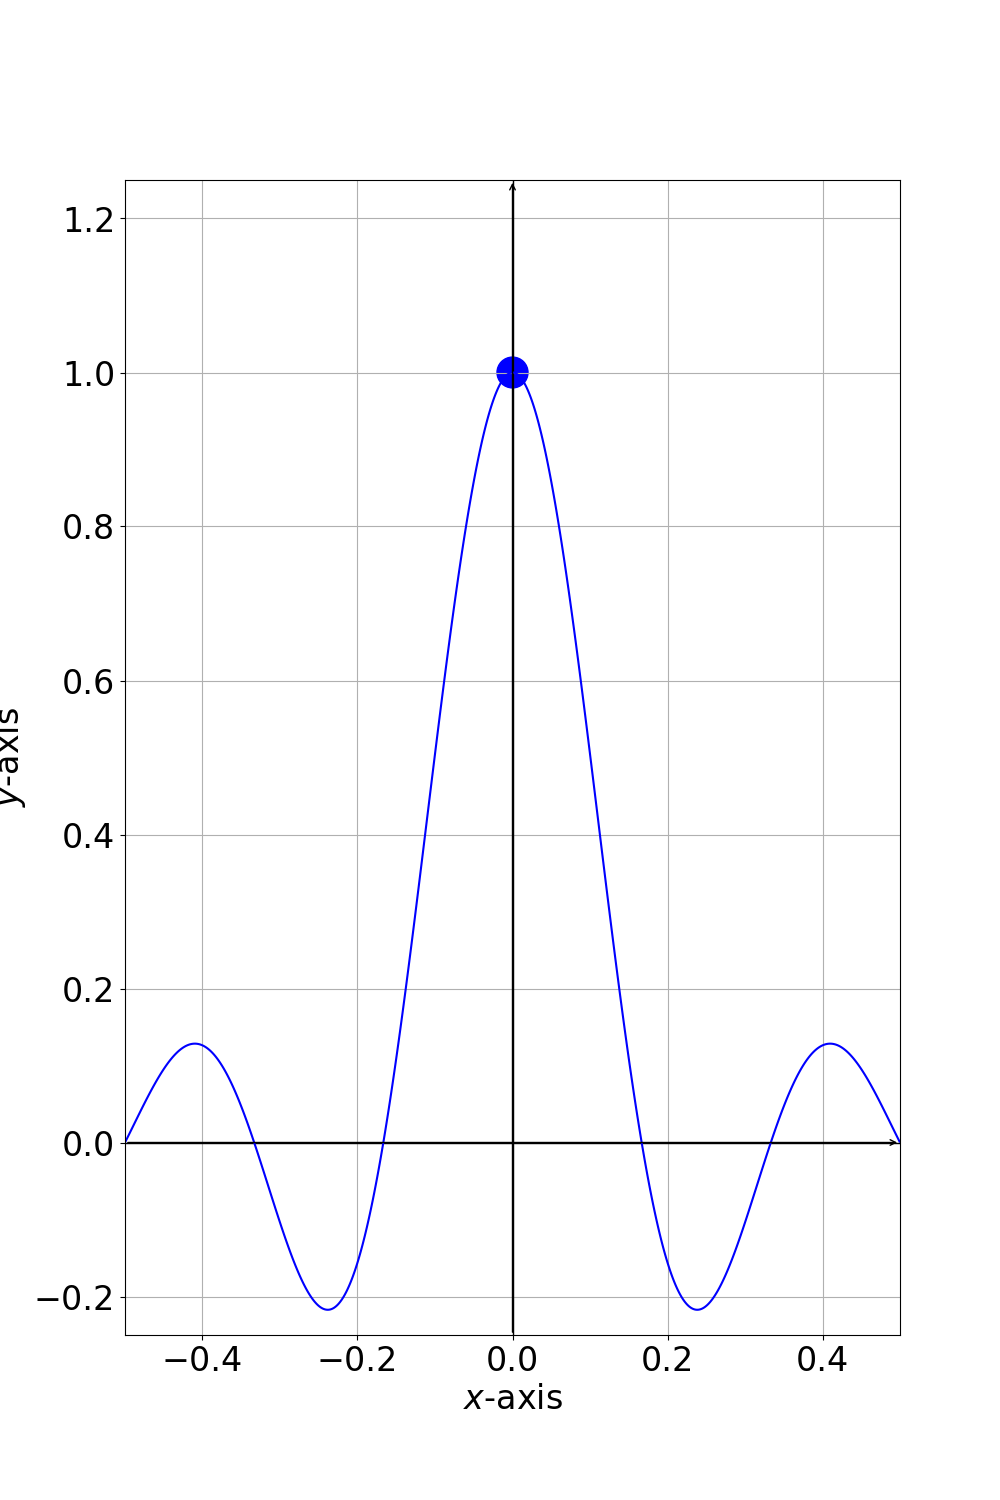
\includegraphics[width=0.32\textwidth]{defined_or_not_1.png}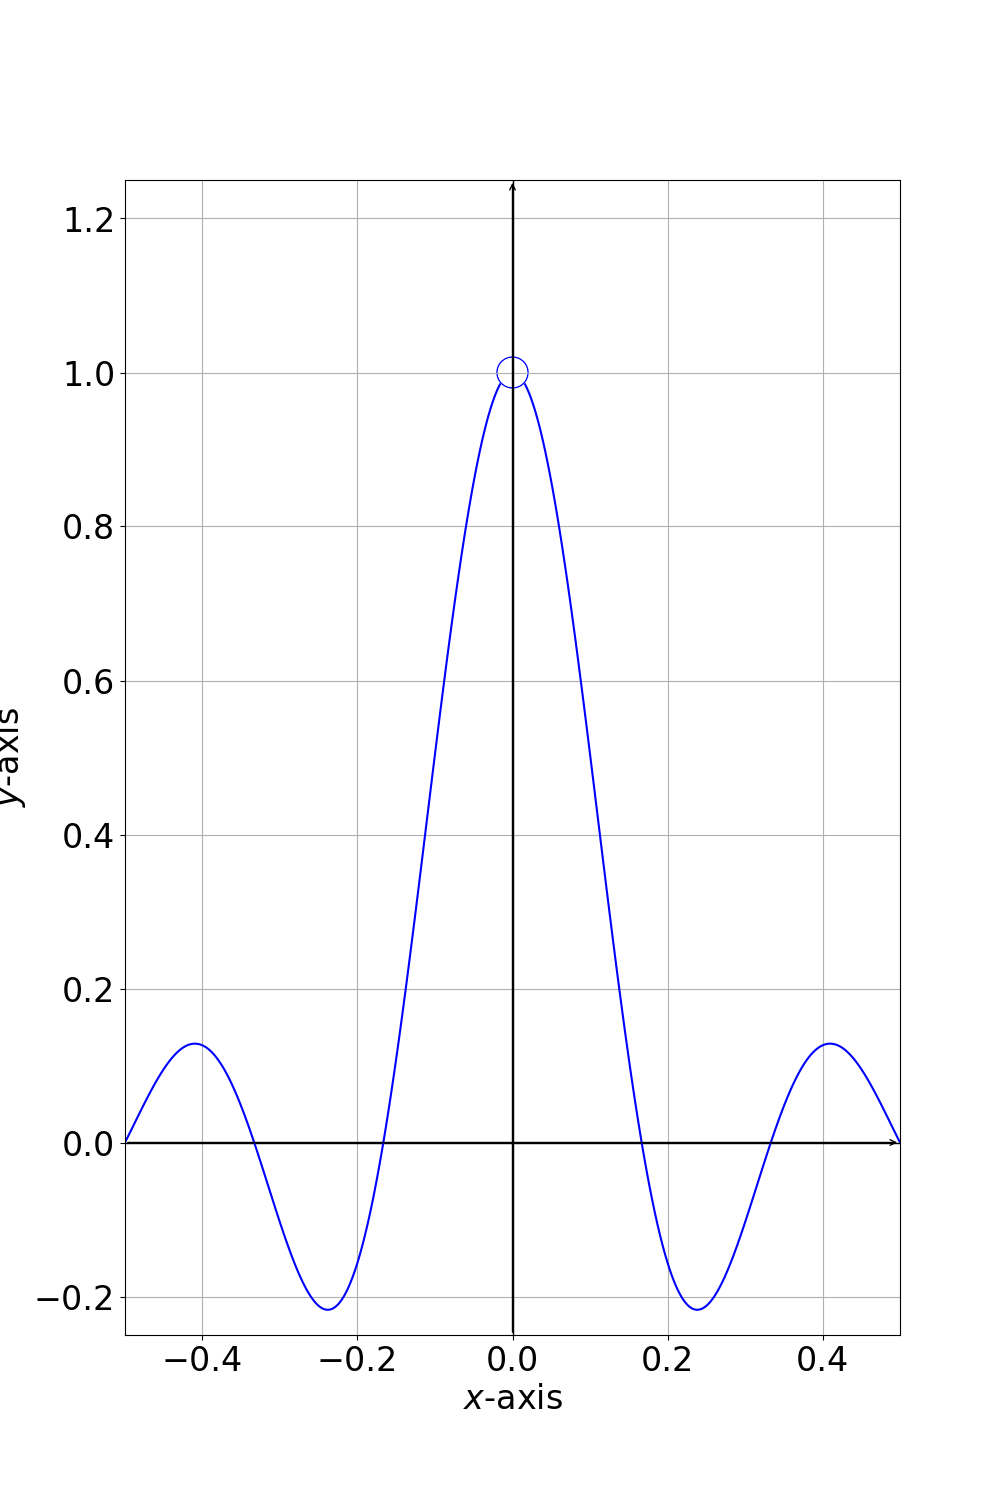
\includegraphics[width=0.32\textwidth]{defined_or_not_2.png}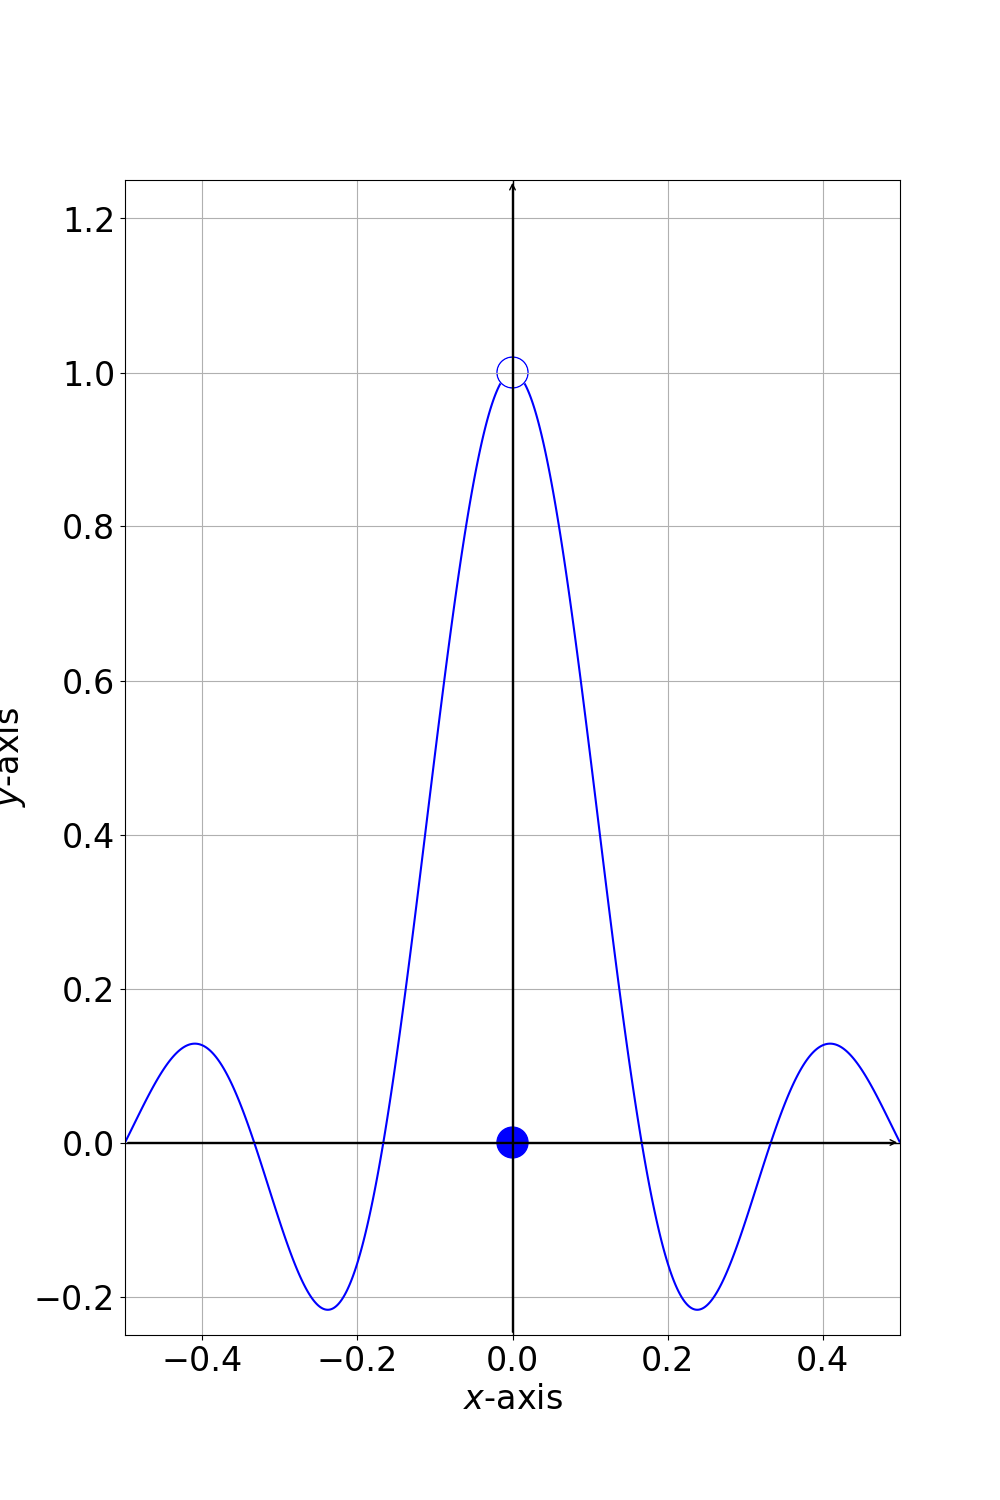
\includegraphics[width=0.32\textwidth]{defined_or_not_3.png}\figtag{2.1.1}
\end{center}

The first case is that the value of the function equals the limit $f(0)=1$. The second case is that $f$ is not defined at $0$. The third case is that the value of the function does not equal the limit $f(0)\ne 1$. However, in these three cases, $$\lim_{x\to 0}f(x)=1.$$

\begin{example}
    Find $\displaystyle\lim_{x\to c_i}f_i(x)$ for the following.
    \begin{enumerate}
        \item $f_1(x)=\dfrac{x^2-9}{x-3}, \quad c_1=3$.
        \item $f_2(x)=\dfrac{x^3-8}{x-2}, \quad c_2=2$.
    \end{enumerate}
\end{example}
\textbf{Solution}. For $\displaystyle\lim_{x\to c_1}f_1(x)$, the function $f_1$ is not defined at $3$. However, to find the limit at $3$, it does not matter whether $f_1$ is defined at $3$ or not. We just care about $f_1$ near $3$ but not equal to $3$. For $x\ne 3$, $\dfrac{x^2-9}{x-3}=x+3$. Hence, $\displaystyle\lim_{x\to 3}\dfrac{x^2-9}{x-3}=\lim_{x\to 3}x+3=6$. For $\displaystyle\lim_{x\to c_2}f_2(x)$, the function $f_2$ is not defined at $2$. However, for $x\ne 2$, $\dfrac{x^3-8}{x-2}=x^2+2x+4$. Hence, $\displaystyle\lim_{x\to 2}\dfrac{x^3-8}{x-2}=\lim_{x\to 2}x^2+2x+4=12$. \qed

One can make $x$ approach $c$ either from the right side or from the left side. Sometimes, a function cannot have a limit with approaches from both sides. The ``one-sided limits'' may exist. We write $$\lim_{x\to c^-}f(x)=L$$ to indicate that $f(x)$ approaches $L$ when $x$ approaches $c$ from the left, and we write $$\lim_{x\to c^+}f(x)=L$$ to indicate that $f(x)$ approaches $L$ when $x$ approaches $c$ from the right.

\begin{example}
    Find the left-hand-side limit $\displaystyle\lim_{x\to 2^-}f(x)$ and the right-hand-side limit $\displaystyle\lim_{x\to 2^+}f(x)$ in Figure 2.1.2. Note that $f$ is not defined at $2$.
\end{example}
\textbf{Solution}. From the figure, we have $\displaystyle\lim_{x\to 2^-}f(x)=1$ and $\displaystyle\lim_{x\to 2^+}f(x)=-1$. \qed

For a limit to exist, both the left-hand-side limit and the right-hand-side limit must exist and equal.

\begin{example}
    Let $f(x)=\dfrac{x}{|x|}$ defined on $(-\infty, 0)\cup(0, \infty)$. Note that $f(x)=1$ for $x>0$ and $f(x)=-1$ for $x<0$. Find the two one-sided limits of $f$ at $0$ and show that the limit of $f$ at $0$ does not exist.
\end{example}
\textbf{Solution}. Since $f(x)=1$ for $x>0$, we easily have $\displaystyle\lim_{x\to 0^+}f(x)=1$ regardless of the fact that $f$ is not defined at $0$. Similarly, $\displaystyle\lim_{x\to 0^-}f(x)=-1$. Since the left-hand-side limit and the right-hand-side limit are not equal, the limit does not exist. \qed

\begin{center}
    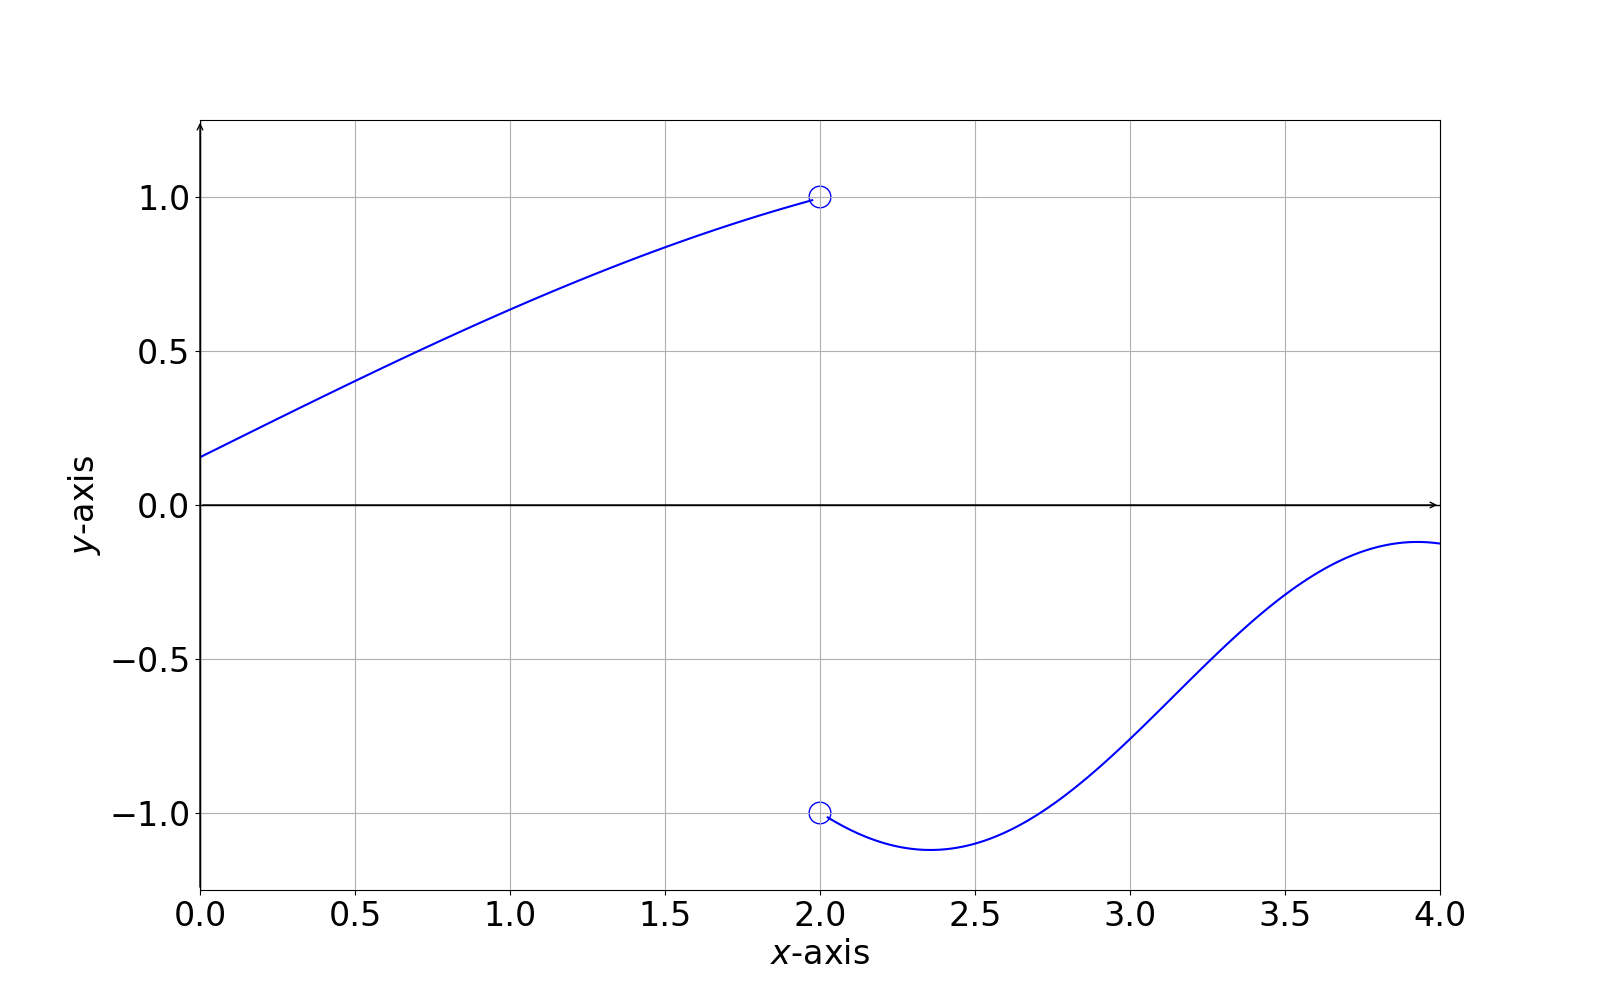
\includegraphics[width=0.6\textwidth]{jumpy.png}\figtag{2.1.2}
\end{center}

\begin{remark}
    For a limit to exist, it must be finite. Otherwise, we say the limit does not exist. However, if a limit does not exist, it might be either oscillating or unbounded (infinite).
\end{remark}

\begin{example}
    In Figure 2.1.3, the limits $\displaystyle\lim_{x\to 3} f(x)$ and $\displaystyle\lim_{x\to 9} f(x)$ do not exist since the function is unbounded near $3$ and $9$.
\end{example}

\begin{example}
    In Figure 2.1.4, the graph of $f(x)=\dfrac{1}{x-2}$ is depicked. As $x$ approaches $4$, $\dfrac{1}{x-2}$ approaches $\dfrac{1}{2}$. Hence, $\displaystyle\lim_{x\to 4}\dfrac{1}{x-2}=\dfrac{1}{2}$. However, as approaches $2$, $\dfrac{1}{x-2}$ gets larger and larger, and $\dfrac{1}{x-2}$ is hence unbounded.
\end{example}

\begin{example}
    Let $$f(x)=\left\{\begin{array}{rl}
        1-x^2, \quad & \text{if $x<1$},\\\dfrac{1}{x-1}, \quad & \text{if $x>1$}.
    \end{array}\right.$$ Find the two one-sided limits of $f$ at $1$ and show that the limit of $f$ at $1$ does not exist.
\end{example}
\textbf{Solution}. For $x<1$, $f(x)=1-x^2$. Thus, $$\lim_{x\to1^-}f(x)=0.$$ For $x>1$, $f(x)=\dfrac{1}{x-1}$. Thus, as $x$ approaches $1$ from the right side, $f(x)$ get larger and larger, and $\dfrac{1}{x-1}$ is hence unbounded. Therefore, $\displaystyle\lim_{x\to 1}f(x)$ does not exist.

\begin{center}
    \begin{minipage}{0.485\textwidth}
        \begin{center}
            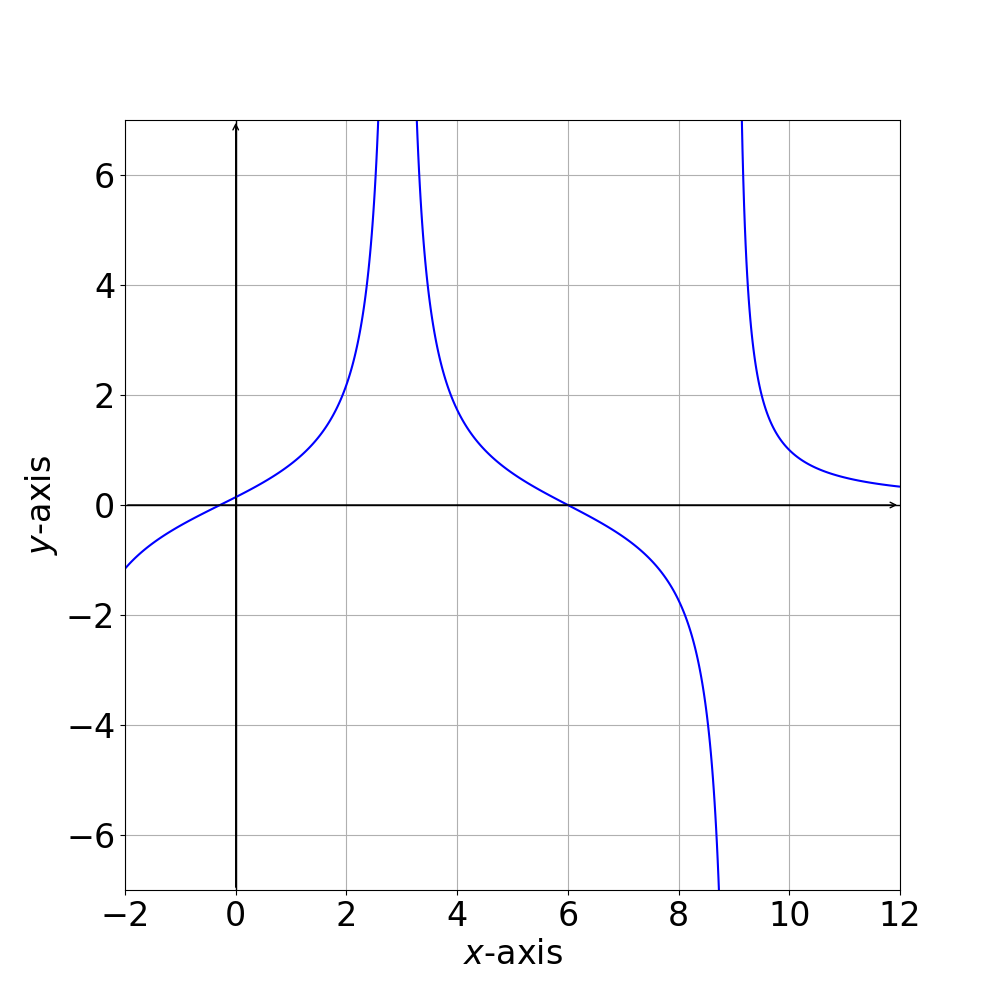
\includegraphics[width=0.85\textwidth]{critical.png}\figtag{2.1.3}
        \end{center}
    \end{minipage}
    \begin{minipage}{0.485\textwidth}
        \begin{center}
            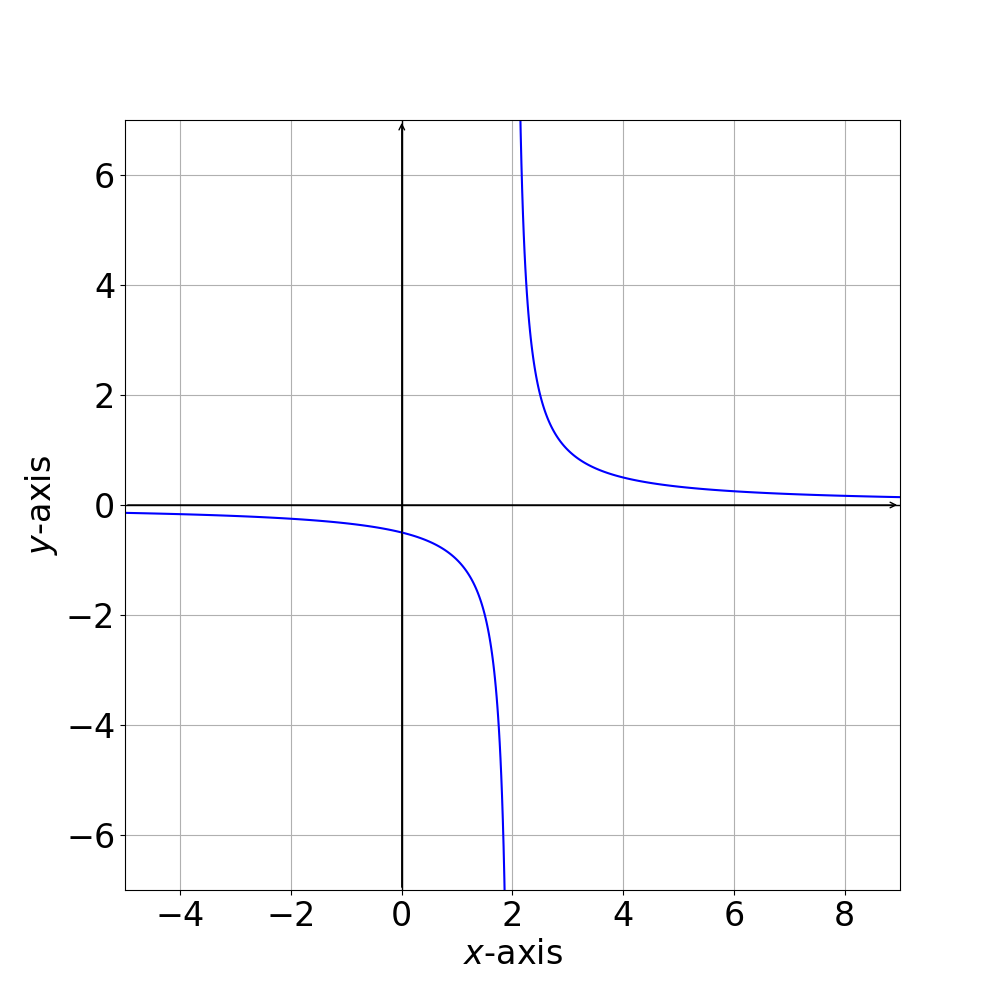
\includegraphics[width=0.85\textwidth]{limit_reciprocal.png}\figtag{2.1.4}
        \end{center}
    \end{minipage}
\end{center}

\subsection*{Exercise}

\begin{enumerate}[label=\arabic*.]
    \item Find $\displaystyle\lim_{x\to c^-}f(x), \lim_{x\to c^+}f(x), \lim_{x\to c}f(x), f(c)$ with the given graph of $f$ and number $c$.
    \begin{multicols}{2}
        \begin{enumerate}
            \item $c=2$.\\
            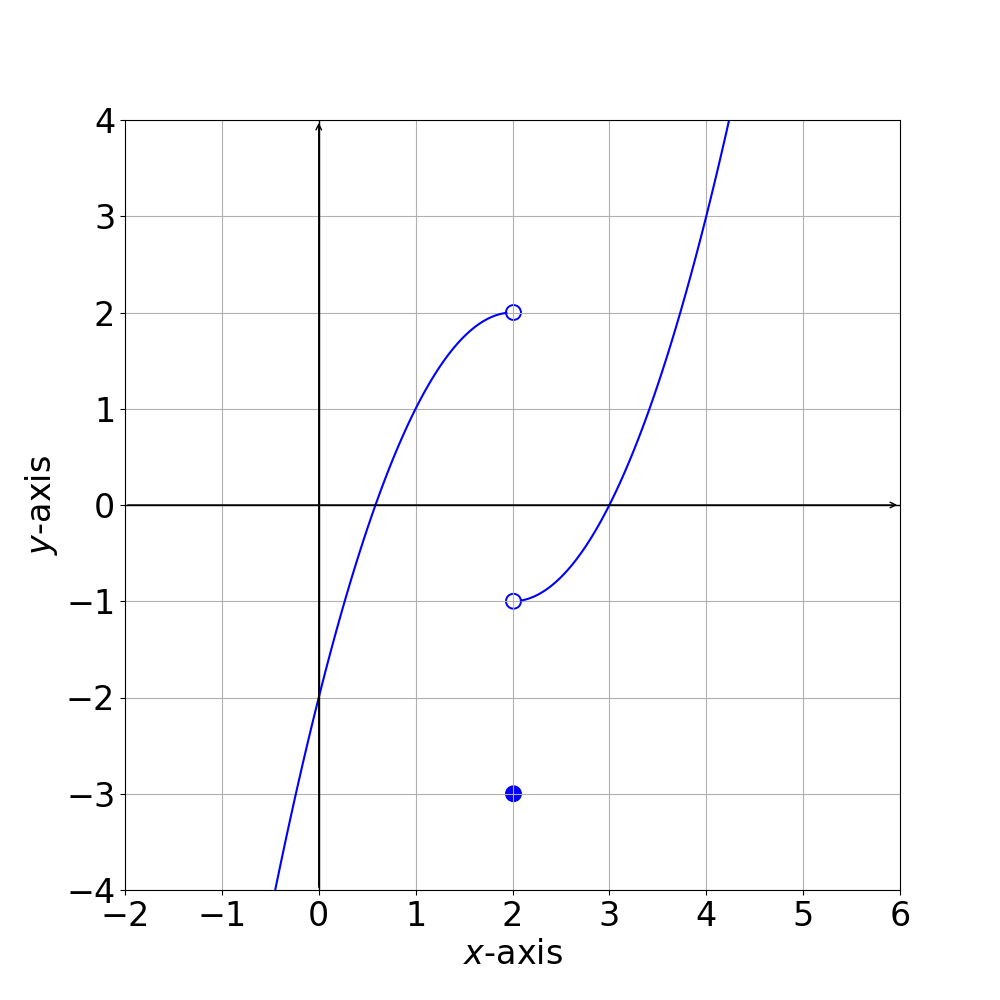
\includegraphics[width=0.41\textwidth]{limit_ex_1.png}\\
            \phantom{\ }
            \item $c=3$.\\
            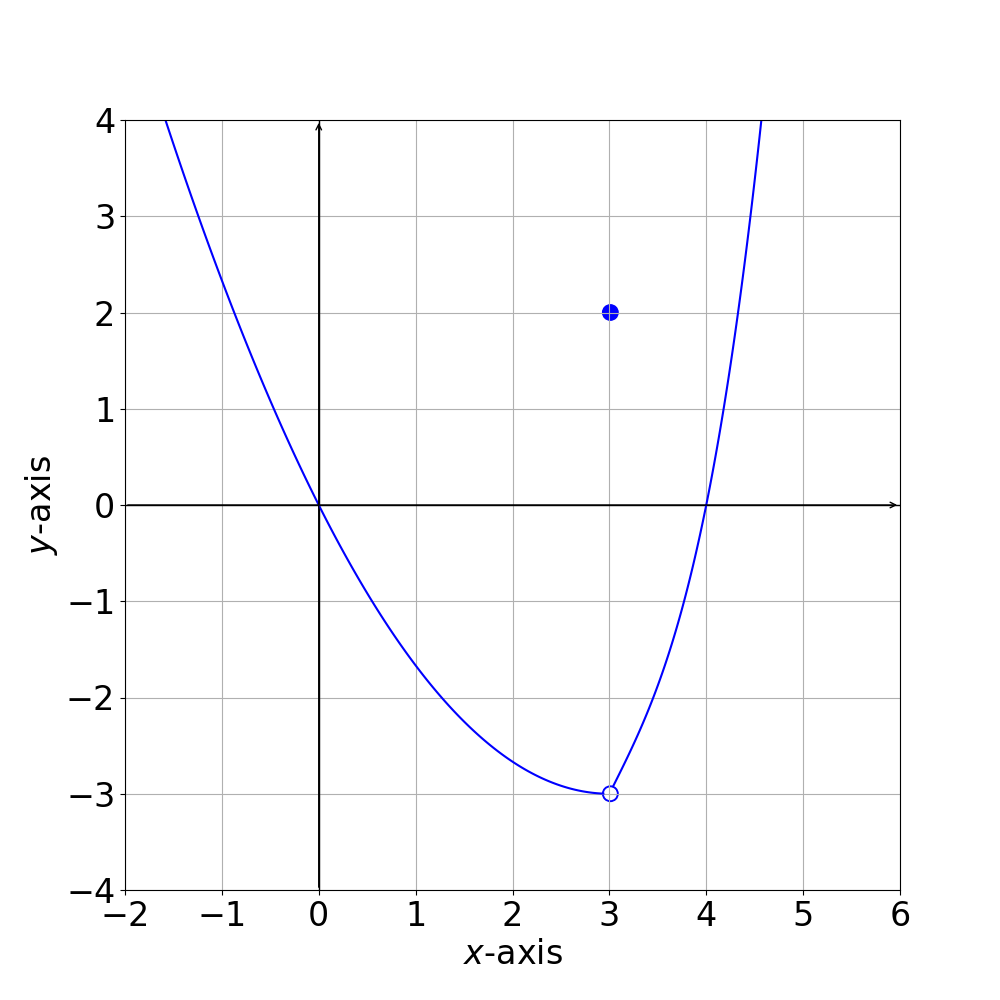
\includegraphics[width=0.41\textwidth]{limit_ex_2.png}\\
            \phantom{\ }
            \item $c=3$.\\
            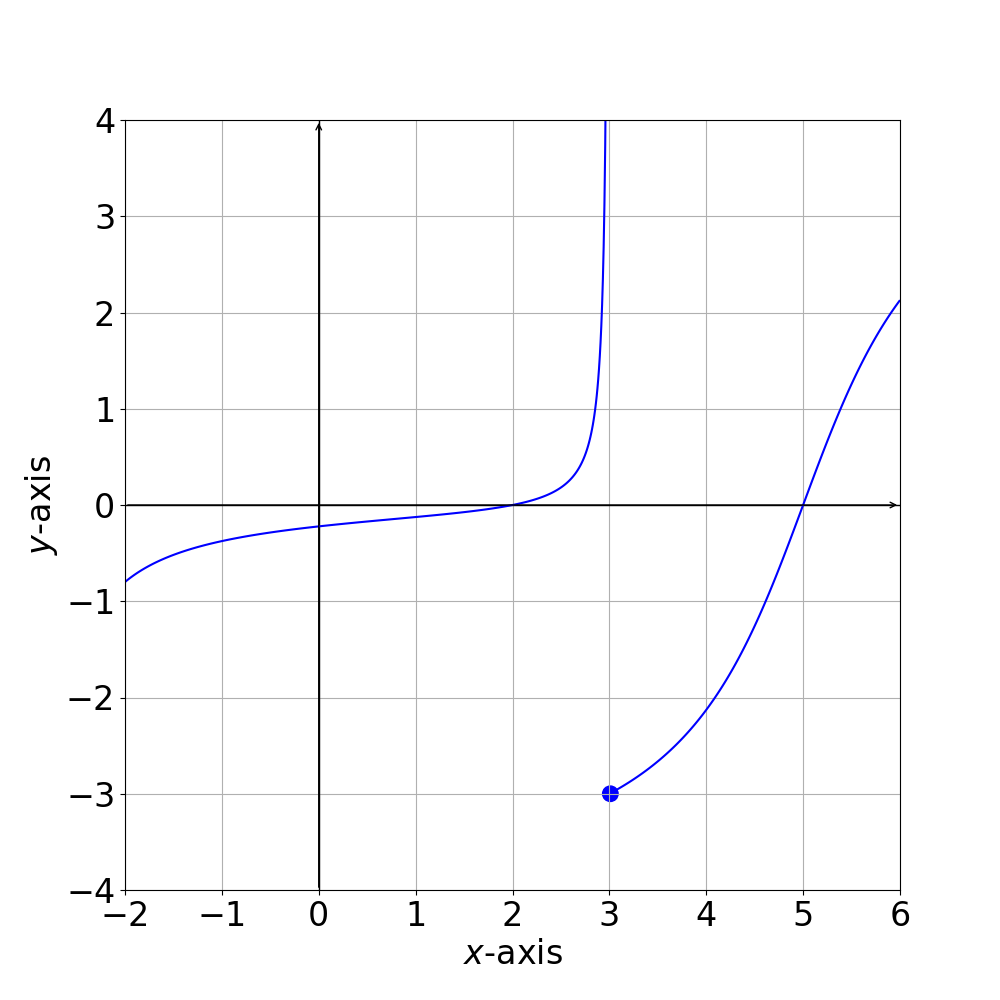
\includegraphics[width=0.41\textwidth]{limit_ex_3.png}
            \item $c=4$.\\
            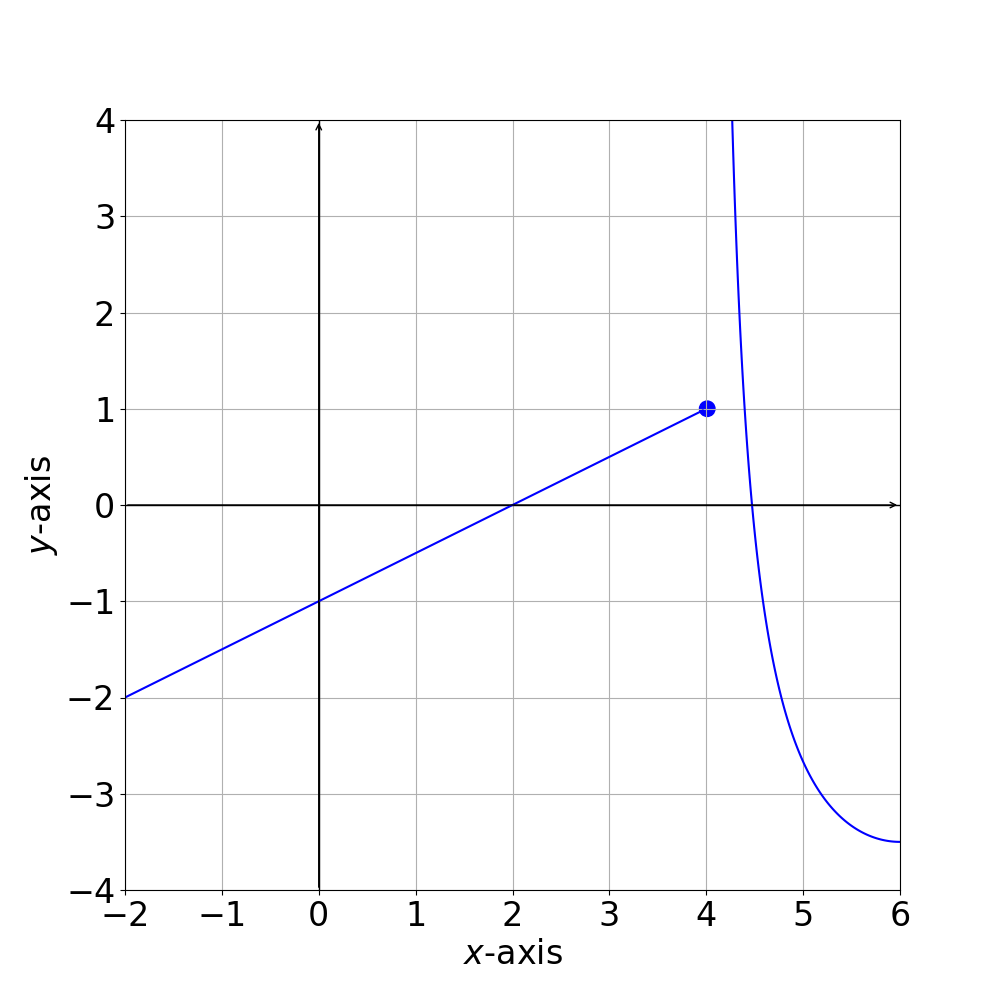
\includegraphics[width=0.41\textwidth]{limit_ex_4.png}
            \item $c=-2$.\\
            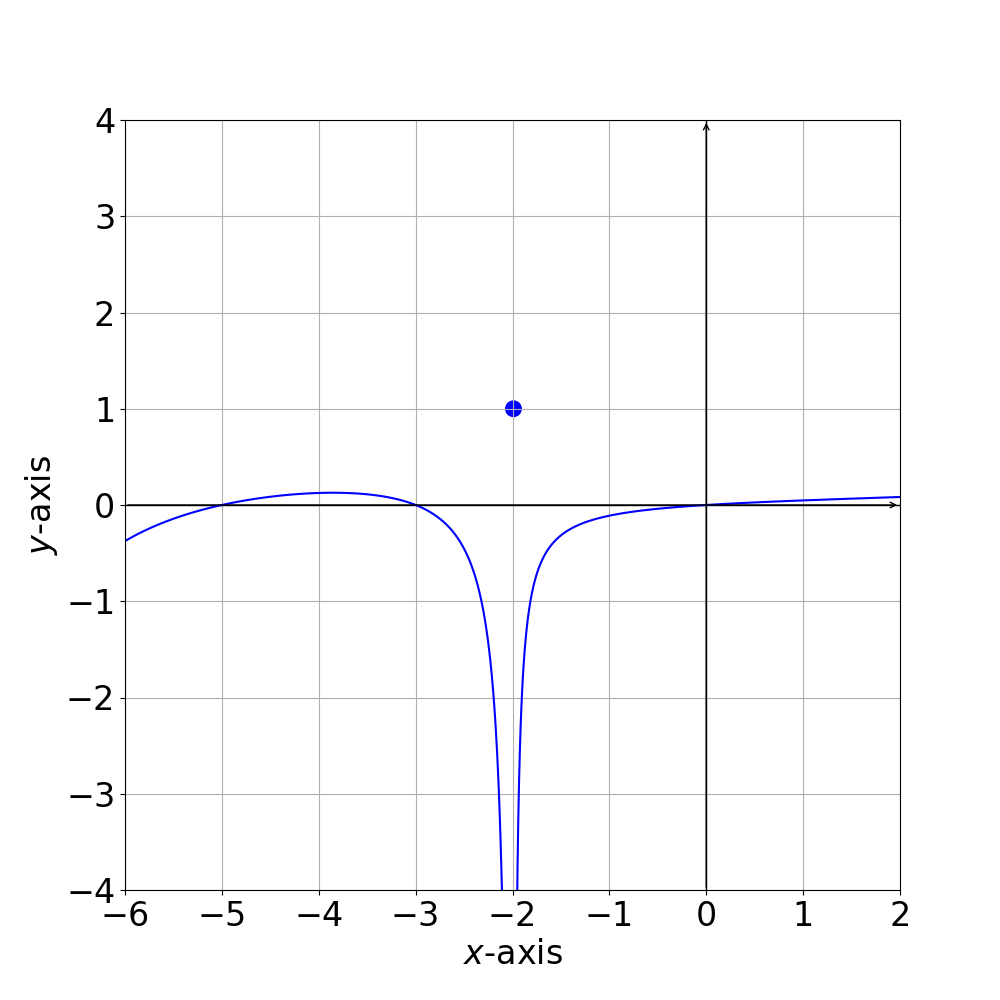
\includegraphics[width=0.41\textwidth]{limit_ex_5.png}
            \item $c=1$.\\
            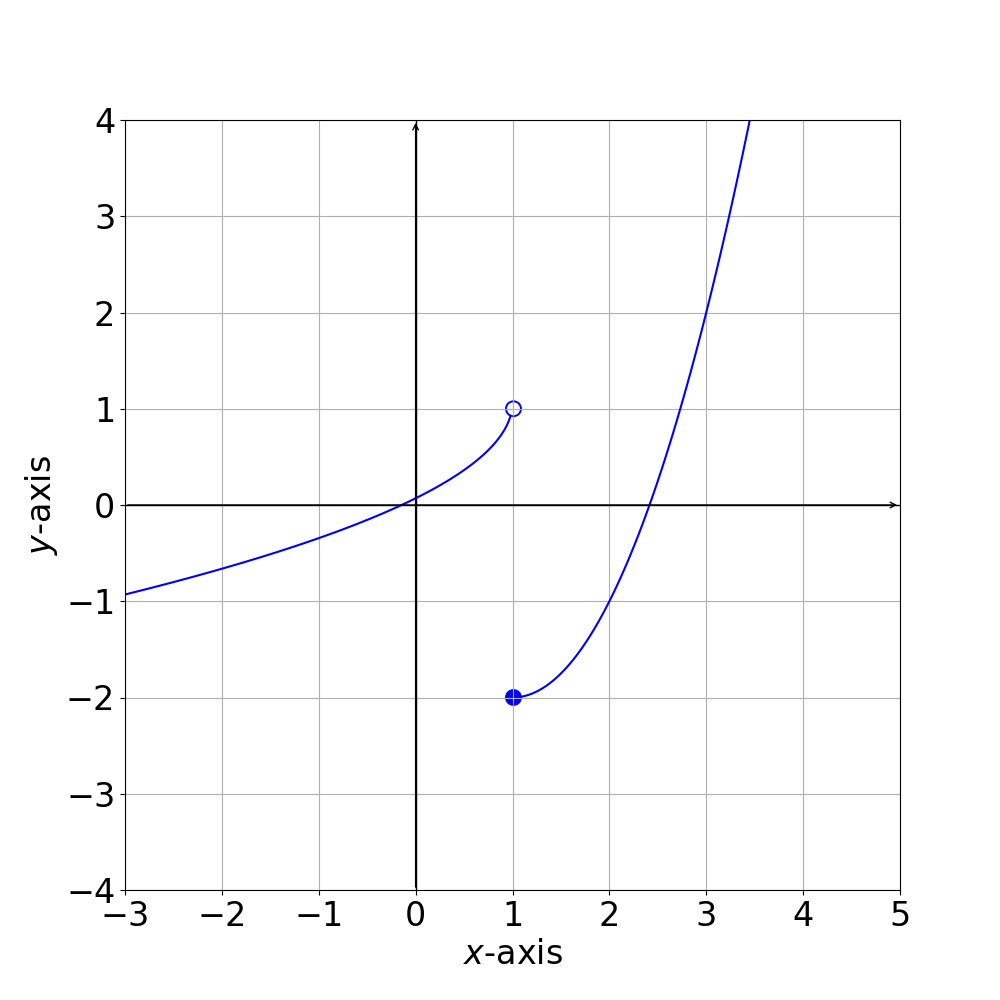
\includegraphics[width=0.41\textwidth]{limit_ex_6.png}
        \end{enumerate}
    \end{multicols}
    \item Decide on intuitive grounds whether the indicated limit exists. Evaluate it if it exists.
    \begin{enumerate}
        \begin{multicols}{2}
            \item $\displaystyle\lim_{x\to 2}2x-1$.
            \item $\displaystyle\lim_{x\to-2}x^2-2x+4$.
            \item $\displaystyle\lim_{x\to 1}2-5x$.
            \item $\displaystyle\lim_{x\to 0}\dfrac{1}{|x|}$.
            \item $\displaystyle\lim_{x\to 3}\dfrac{2x-6}{x-3}$.
            \item $\displaystyle\lim_{x\to 1}x+\dfrac{1}{x}$.
            \item $\displaystyle\lim_{x\to 1}\dfrac{x^2-1}{x-1}$.
            \item $\displaystyle\lim_{x\to 1}\dfrac{x^3-1}{x-1}$.
            \item $\displaystyle\lim_{x\to 1}\dfrac{x^3-1}{x+1}$.
            \item $\displaystyle\lim_{x\to 1}\dfrac{x^2+1}{x^2-1}$.
        \end{multicols}
        \item $\displaystyle\lim_{x\to 0}f(x)$ with $f(x)=\left\{\begin{array}{rl}
            1, \quad & \text{if $x\ne0$},\\
            3, \quad & \text{if $x=0$}.
        \end{array}\right.$
        \item $\displaystyle\lim_{x\to 1}f(x)$ with $f(x)=\left\{\begin{array}{rl}
            3x, \quad & \text{if $x<1$},\\
            3, \quad & \text{if $x>1$}.
        \end{array}\right.$
        \item $\displaystyle\lim_{x\to 4}f(x)$ with $f(x)=\left\{\begin{array}{rl}
            x^2, \quad & \text{if $x\ne4$},\\
            0, \quad & \text{if $x=4$}.
        \end{array}\right.$
        \item $\displaystyle\lim_{x\to 0}f(x)$ with $f(x)=\left\{\begin{array}{rl}
            -x^2, \quad & \text{if $x<0$},\\
            x^2, \quad & \text{if $x>0$}.
        \end{array}\right.$
        \item $\displaystyle\lim_{x\to 0}f(x)$ with $f(x)=\left\{\begin{array}{rl}
            x^2, \quad & \text{if $x<0$},\\
            1+x, \quad & \text{if $x>0$}.
        \end{array}\right.$
        \item $\displaystyle\lim_{x\to 1}f(x)$ with $f(x)=\left\{\begin{array}{rl}
            2x, \quad & \text{if $x<1$},\\
            x^2+1, \quad & \text{if $x>1$}.
        \end{array}\right.$
        \item $\displaystyle\lim_{x\to 0}f(x)$ with $f(x)=\left\{\begin{array}{rl}
            1, \quad & \text{if $x\in\mathbb{Q}$},\\
            -1, \quad & \text{if $x\notin\mathbb{Q}$}.
        \end{array}\right.$
        \item $\displaystyle\lim_{x\to 1}f(x)$ with $f(x)=\left\{\begin{array}{rl}
            2x, \quad & \text{if $x\in\mathbb{Q}$},\\
            2, \quad & \text{if $x\notin\mathbb{Q}$}.
        \end{array}\right.$
    \end{enumerate}
\end{enumerate}

\section{Definition of Limit}

Just as previously stated, the limit cares about the behavior of the function $f$ near a point $c$. We say the limit of $f$ at $c$ is $L$ if the value of the function $f(x)$ gets closer to $L$ as $x$ approaches $c$. More generally speaking, we say the limit of $f$ at $c$ is $L$ if the difference between $f(x)$ and $L$ can be assured to be arbitrarily small as $x$ and $c$ are closed enough.

The difference between $f(x)$ and $L$ can be described in mathematical language: $|f(x)-L|$. We want the error of function to be arbitrarily small, say we want the error to be less than $\varepsilon$. We just easily have the inequality $|f(x)-L|<\varepsilon$.

Let's say number $a$ and number $b$ are closed enough if their distance is less than $\delta$. Now, we can use interval to show that $x$ and $c$ are closed enough: $x\in(c-\delta, c)\cup(c, c+\delta)$. This is almost our definition of the limit.

\begin{definition}[Limit]
    Let $f:A\to\bbR$ be a function, where $A\subseteq\bbR$. Let $L\in\bbR$ and $c\in A$. We say the \underline{limit} of $f$ at $c$ is $L$ if for all $\varepsilon>0$, there exists a $\delta>0$ such that $0<|x-c|<\delta$ implies $|f(x)-L|<\varepsilon$. In this case, we write $\displaystyle\lim_{x\to c}f(x)=L$.
\end{definition}

\begin{remark}
    Usually, the choice of $\delta$ depends on $\varepsilon$. The definition does not require a unique difference $\delta$ to work for all error $\varepsilon$, which is quite impossible. Since the error $\varepsilon$ is given before the choice of $\delta$, if we know that a number $\delta_0$ will work as a $\delta$, then any positive number less than $\delta_0$ will work as the interval is smaller.
\end{remark}

\begin{example}
    Show that $$\lim_{x\to 1}2x+1=3.$$
\end{example}
\textit{Sketch of the proof}. We need to find a $\delta$ with connection to $\varepsilon$ such that $|x-1|<\delta$ implies $|2x+1-3|<\varepsilon$. Observe that $|2x+1-3|=2|x-1|$. Now, the question becomes easier, and we just need to select a $\delta$ with the following two inequalities: 
\begin{equation*}
    |x-1|<\delta, \qquad\text{and}\qquad 2|x-1|<\varepsilon.
\end{equation*}
A natural choice is $\delta=\dfrac{\varepsilon}{2}$. However, just like previously stated, any number less than $\dfrac{\varepsilon}{2}$ will work, such as $\dfrac{\varepsilon}{3}, \dfrac{\varepsilon}{4}$.\\
\textbf{Proof}. Let $\varepsilon>0$. Choose $\delta=\dfrac{\varepsilon}{2}$. Then, $0<|x-1|<\delta=\dfrac{\varepsilon}{2}$ implies $|2x+1-3|=2|x-1|<2\cdot\dfrac{\varepsilon}{2}=\varepsilon$. \qed

The proof itself is quite straightforward, but the work beforehand is the essence of the definition.

\begin{example}
    Show that $$\lim_{x\to -1}2-3x=5.$$
\end{example}
\textit{Sketch of the proof}. We need to find a $\delta$ with connection to $\varepsilon$ such that $|x-(-1)|<\delta$ implies $|2-3x-5|<\varepsilon$. Observe that $|2-3x-5|=3|x+1|$. Now, the question becomes easier, and we just need to select a $\delta$ with the following two inequalities: 
\begin{equation*}
    |x+1|<\delta, \qquad\text{and}\qquad 3|x+1|<\varepsilon.
\end{equation*}
A natural choice is $\delta=\dfrac{\varepsilon}{3}$. However, just like previously stated, any number less than $\dfrac{\varepsilon}{3}$ will work.\\
\textbf{Proof}. Let $\varepsilon>0$. Choose $\delta=\dfrac{\varepsilon}{3}$. Then, $0<|x+1|<\delta=\dfrac{\varepsilon}{3}$ implies $|2-3x-5|=3|x+1|<3\cdot\dfrac{\varepsilon}{3}=\varepsilon$. \qed

\begin{proposition}
    Let $c\in\bbR$. Then, $$\lim_{x\to c}x=c.$$
\end{proposition}
\textbf{Proof}. Let $\varepsilon>0$. Choose $\delta=\varepsilon$. Then, $0<|x-c|<\delta=\varepsilon$ implies $|x-c|<\varepsilon$. \qed

\begin{proposition}
    Let $c\in\bbR$ and $r\in\bbR$. Then, $$\lim_{x\to c}r=r.$$
\end{proposition}
\textbf{Proof}. Let $\varepsilon>0$. Choose $\delta$ to be an arbitrary positive number. Then, $|r-r|=0<\varepsilon$. \qed

\begin{proposition}
    Let $c\in\bbR$. Then, $$\lim_{x\to c}|x|=|c|.$$
\end{proposition}
\textbf{Proof}. Let $\varepsilon>0$. Choose $\delta=\varepsilon$. Then, $0<|x-c|<\delta=\varepsilon$ implies $||x|-|c||\leq|x-c|<\varepsilon$. \qed

In fact, we can prove the limit and the value of the function is the same for every polynomial. We now prove the case when the degree is $1$.

\begin{proposition}
    Let $a\ne 0$ and $b\in\bbR$. Let $c\in\bbR$. Then, $$\lim_{x\to c}ax+b=ac+b.$$
\end{proposition}
\textbf{Proof}. Let $\varepsilon>0$. Choose $\delta=\dfrac{\varepsilon}{|a|}$. Then, $0<|x-c|<\delta=\dfrac{\varepsilon}{|a|}$ implies $|ax+b-ac+b|=|a||x-c|<|a|\cdot\dfrac{\varepsilon}{|a|}=\varepsilon$. \qed

\begin{remark}
    If $a\in\bbR$, we just choose $\delta=\dfrac{\varepsilon}{1+|a|}$ to avoid devided by $0$ generally, or we treat two cases differently.
\end{remark}

\begin{proposition}
    Let $c\in\bbR$. Then, $$\lim_{x\to c}x^2=c^2.$$
\end{proposition}
\textit{Sketch of the proof}. We need to find a $\delta$ with connection to $\varepsilon$ such that $|x-c|<\delta$ implies $|x^2-c^2|<\varepsilon$. Observe that $|x^2-c^2|=|x+c||x-c|$. We need to eliminate the term $|x+c|$ to get an easier relation. Since we want $x$ to approach $c$, we may first set $|x-c|<1$. We choose $1$ since it is a number that we are familiar with. One can choose any other positive number. Now, we can estimate the range of $|x+c|$ when $|x-c|<1$. If $|x-c|<1$, it means that $x\in(c-1, c+1)$. Hence, the range of $|x+c|$ is $(2c-1, 2c+1)$. Hence, we know that $|x+c|<\max\{2c-1, 2c+1\}\leq 2|c|+1$. We now just need to select a $\delta$ with the following two inequalities: 
\begin{equation*}
    |x-c|<\delta, \qquad\text{and}\qquad |x+c||x-c|<(2|c|+1)|x-c|<\varepsilon.
\end{equation*}
A natural choice is $\delta=\dfrac{\varepsilon}{2|c|+1}$. One has to remember that we set $|x-c|<1$. So we need to choose $\delta$ that is less than $1$.\\\setlength{\delimitershortfall}{0pt}
\textbf{Proof}. Let $\varepsilon>0$. Choose $\delta=\min\left\{1, \dfrac{\varepsilon}{2|c|+1}\right\}$. Then, $0<|x-c|<\delta=$ implies \begin{align*}
    |x^2-c^2|&=|x+c||x-c|\\
    &<(2|c|+1)\cdot\min\left\{1, \dfrac{\varepsilon}{2|c|+1}\right\}\\
    &\leq\varepsilon.
\end{align*} \qed

\setlength{\delimitershortfall}{13.5pt}

\begin{proposition}
    Let $c\in(0, \infty)$. Then, $$\lim_{x\to c}\sqrt{x}=\sqrt{c}.$$
\end{proposition}
\textbf{Proof}. Let $\varepsilon>0$. Choose $\delta=\sqrt{c}\varepsilon$. Then, $0<|x-c|<\delta=\sqrt{c}\varepsilon$ implies

\begin{align*}
    |\sqrt{x}-\sqrt{c}|&=\dfrac{|x-c|}{\sqrt{x}+\sqrt{c}}\\
    &\leq\dfrac{|x-c|}{\sqrt{c}}\\
    &<\dfrac{\sqrt{c}\varepsilon}{\sqrt{c}}\\
    &=\varepsilon.
\end{align*} \qed

\begin{theorem}
    The following are equivalent.
    \vspace{-1.2em}
    \begin{multicols}{2}
        \begin{enumerate}
            \item $\displaystyle\lim_{x\to c}f(x)=L$.
            \item $\displaystyle\lim_{h\to 0}f(x+h)=L$.
            \item $\displaystyle\lim_{x\to c}f(x)-L=0$.
            \item $\displaystyle\lim_{x\to c}|f(x)-L|=0$.
        \end{enumerate}
    \end{multicols}
    \vspace{0.01em}
\end{theorem}

We can use the same language to construct the two one-sided limits, and state that the limit exists if and only if the two one-sided limits exist and are equal. Note that the two $\delta$'s might not be equal if you are only given that two one-sided limits exists and are equal.

\begin{definition}[Left-Hand-Side Limit]
    Let $f:A\to\bbR$ be a function, where $A\subseteq\bbR$. Let $L\in\bbR$ and $c\in A$. We say the \underline{left-hand-side limit} of $f$ at $c$ is $L$ if for all $\varepsilon>0$, there exists a $\delta>0$ such that $0<c-x<\delta$ implies $|f(x)-L|<\varepsilon$. In this case, we write $\displaystyle\lim_{x\to c^-}f(x)=L$.
\end{definition}

\begin{definition}[Right-Hand-Side Limit]
    Let $f:A\to\bbR$ be a function, where $A\subseteq\bbR$. Let $L\in\bbR$ and $c\in A$. We say the \underline{right-hand-side limit} of $f$ at $c$ is $L$ if for all $\varepsilon>0$, there exists a $\delta>0$ such that $0<x-c<\delta$ implies $|f(x)-L|<\varepsilon$. In this case, we write $\displaystyle\lim_{x\to c^+}f(x)=L$.
\end{definition}

\begin{theorem}
    Let $f:A\to\bbR$ be a function, where $A\subseteq\bbR$. Let $L\in\bbR$ and $c\in A$. The limit $\displaystyle\lim_{x\to c}f(x)=L$ if and only if $\displaystyle\lim_{x\to c^-}f(x)=L$ and $\displaystyle\lim_{x\to c^-}f(x)=L$.
\end{theorem}

\begin{example}
    Evaluate $\displaystyle\lim_{x\to 1}f(x)$ for function $f$ defined by $$f(x)=\left\{\begin{array}{rl}
        1+x^2, \quad & \text{if $x<1$},\\
        3, \quad & \text{if $x=1$},\\
        4-2x, \quad & \text{if $x>1$}.
    \end{array}\right.$$
\end{example}
\textbf{Solution}. The left-hand-side limit $$\lim_{x\to 1^-}f(x)=\lim_{x\to 1^-}4-2x=2$$ and the right-hand-side limit $$\lim_{x\to 1^+}f(x)=\lim_{x\to 1^+}4-2x=2$$ are equal. Hence, the limit $\displaystyle\lim_{x\to 1}f(x)=2$. \qed

\subsection*{Exercise}

\begin{enumerate}[label=\arabic*.]
    \item Decide whether the indicated limit exists. Evaluate it if it exists.
    \begin{enumerate}
        \begin{multicols}{4}
            \item $\displaystyle\lim_{x\to 1}\dfrac{x}{x+1}$.
            \item $\displaystyle\lim_{x\to 0}\dfrac{x^2(1+x)}{2x}$.
            \item $\displaystyle\lim_{x\to 0}\dfrac{x^2(1+x)}{2x^2}$.
            \item $\displaystyle\lim_{x\to 4}\dfrac{x}{\sqrt{x}+1}$.
            \item $\displaystyle\lim_{x\to 1}\dfrac{x^4-1}{x-1}$.
            \item $\displaystyle\lim_{x\to -2}\dfrac{x}{|x|}$.
            \item $\displaystyle\lim_{x\to -1}\dfrac{1-x}{x+1}$.
            \item $\displaystyle\lim_{x\to 3}\dfrac{x-3}{\sqrt{x}-3}$.
            \item $\displaystyle\lim_{x\to 1^+}\dfrac{\sqrt{x-1}}{x}$.
            \item $\displaystyle\lim_{x\to 0^+}\dfrac{x}{|x|}$.
            \item $\displaystyle\lim_{x\to 0^-}\dfrac{x}{|x|}$.
            \item $\displaystyle\lim_{x\to 0}\dfrac{x}{|x|}$.
        \end{multicols}
        \item $\displaystyle\lim_{x\to 2^+}f(x)$ with $f(x)=\left\{\begin{array}{rl}
            2x-1, \quad & \text{if $x\leq 2$},\\
            x^2-x, \quad & \text{if $x>2$}.
        \end{array}\right.$
        \item $\displaystyle\lim_{x\to 2}f(x)$ with $f(x)=\left\{\begin{array}{rl}
            x^2, \quad & \text{if $x<3$},\\
            7, \quad & \text{if $x=3$},\\
            2x+3, \quad & \text{if $x>3$}.
        \end{array}\right.$
        \item $\displaystyle\lim_{x\to 2}f(x)$ with $f(x)=\left\{\begin{array}{rl}
            1, \quad & \text{if $x\in\mathbb{Z}$},\\
            -1, \quad & \text{if $x\notin\mathbb{Z}$}.
        \end{array}\right.$
        \item $\displaystyle\lim_{x\to 0}f(x)$ with $f(x)=\left\{\begin{array}{rl}
            x^2, \quad & \text{if $x\leq 1$},\\
            x, \quad & \text{if $x>1$}.
        \end{array}\right.$
    \end{enumerate}
    \item Find the largest $\delta$ that works for the given $\varepsilon$.
    \begin{multicols}{2}
        \begin{enumerate}
            \item $\displaystyle\lim_{x\to 1}2x=2,\quad \varepsilon=0.1$.
            \item $\displaystyle\lim_{x\to 4}5x=20,\quad \varepsilon=0.5$.
            \item $\displaystyle\lim_{x\to2}\dfrac{x}{2}=1,\quad \varepsilon=0.01$.
            \item $\displaystyle\lim_{x\to2}\dfrac{x}{5}=\dfrac{2}{5},\quad \varepsilon=0.1$.
        \end{enumerate}
    \end{multicols}
\end{enumerate}

\section{Limit Theorems}

We introduce some theorems related to limits here. We will state them and skip the majority of the proof.

\begin{theorem}[Uniqueless of Limit]
    If $\displaystyle\lim_{x\to c}f(x)=L$ and $\displaystyle\lim_{x\to c}f(x)=M$, then $L=M$. That is, the limit of a function at a point is unique.
\end{theorem}

\begin{theorem}[Operations for Limits]\label{lim_op}
    If $\displaystyle\lim_{x\to c}f(x)=L$ and $\displaystyle\lim_{x\to c}g(x)=M$, the following statements hold.
    \begin{enumerate}
        \item $\displaystyle\lim_{x\to c}f(x)+g(x)=L+M$.
        \item $\displaystyle\lim_{x\to c}\alpha\cdot f(x)=\alpha L,\quad \alpha\in\bbR$.
        \item $\displaystyle\lim_{x\to c}f(x)g(x)=LM$.
        \item If $M\ne0$, then $\displaystyle\lim_{x\to c}\dfrac{f(x)}{g(x)}=\dfrac{L}{M}$.
    \end{enumerate}
\end{theorem}

\begin{corollary}
    Let $P$ be a polynomial function. Then, the limit of $P$ at any point $c\in\bbR$ is the value of the function.
\end{corollary}
\textbf{Proof}. Use the two limits $\displaystyle\lim_{x\to c}x=c$ and $\displaystyle\lim_{x\to c}r=r$ with Therorem \ref{lim_op}. \qed

For the special matter in this corollary, the limit equal the value of the function, we say that this kind of functions is continuous. We will talk about this in the next section.

\begin{theorem}
    If $\displaystyle\lim_{x\to c}f(x)=L\ne 0$ and $\displaystyle\lim_{x\to c}g(x)=0$, then $\displaystyle\lim_{x\to c}\dfrac{f(x)}{g(x)}$ does not exist.
\end{theorem}
\textbf{Proof}. Suppose $\displaystyle\lim_{x\to c}\dfrac{f(x)}{g(x)}=M$. On the one hand, since the two limits exist, \begin{align*}
    \lim_{x\to c}\dfrac{f(x)}{g(x)}\cdot g(x)&=\lim_{x\to c}\dfrac{f(x)}{g(x)}\cdot\lim_{x\to c}g(x)\\
    &=M\cdot 0\\
    &=0.
\end{align*} On the other hand, \begin{align*}
    \lim_{x\to c}\dfrac{f(x)}{g(x)}\cdot g(x)&=\lim_{x\to c}f(x)\\
    &=L\\
    &\ne0,
\end{align*} a contradiction. Hence, $\displaystyle\lim_{x\to c}\dfrac{f(x)}{g(x)}$ does not exist. \qed

One have to remember that the numerator must be nonzero; if the numerator and the denominator are both zeros, we cannot apply this theorem.

\begin{example}
    Evaluate the following limits.
    \begin{enumerate}
        \item $\displaystyle\lim_{x\to 2}\dfrac{1/x-1/2}{x-2}$.
        \item $\displaystyle\lim_{x\to 9}\dfrac{x-9}{\sqrt{x}-3}$.
    \end{enumerate}
\end{example}
\textbf{Solution}. For the first expression, \begin{align*}
    \lim_{x\to 2}\dfrac{1/x-1/2}{x-2}&=\lim_{x\to 2}\dfrac{2-x}{2x^2-4x}\\
    &=\lim_{x\to 2}\dfrac{2-x}{2x(x-2)}\\
    &=-\lim_{x\to 2}\dfrac{1}{2x}\\
    &=-\dfrac{1}{4}.
\end{align*} For the second expression, \begin{align*}
    \lim_{x\to 9}\dfrac{x-9}{\sqrt{x}-3}&=\lim_{x\to 9}\dfrac{x-9}{\sqrt{x}-3}\cdot\dfrac{\sqrt{x}+3}{\sqrt{x}+3}\\
    &=\lim_{x\to 9}\dfrac{(x-9)(\sqrt{x}+3)}{|x|-9}\\
    &=\lim_{x\to 9}\sqrt{x}+3\\
    &=6.
\end{align*} The third equation follows since we are looking around $x=9$.\qed

Here comes an extremely important theorem for evaluating trigonometric limits.

\begin{theorem}[Sandwich Theorem]
    Let $f, g, h$ be functions such that $g(x)\leq f(x)\leq h(x)$ for all $x\in(c-\delta, c)\cup(c, c+\delta)$ for some $\delta>0$. If $\displaystyle\lim_{x\to c}g(x)=\lim_{x\to c}h(x)=L$, then $\displaystyle\lim_{x\to c}f(x)=L$.
\end{theorem}

\begin{example}
    In Figure 2.3.1, it can be seen that $0\leq |\sin x|\leq |x|$, where the length of $\tikzarc{AB}$ is $|x|$ and the length of $\overline{AH}$ is $|\sin x|$. Note that the angle between $\overrightarrow{OA}$ and $\overrightarrow{OH}$ is $x$. Using this relation with the sandwich theorem, we can easily have $$\lim_{x\to 0}\sin x=0.$$
\end{example}

\begin{center}
    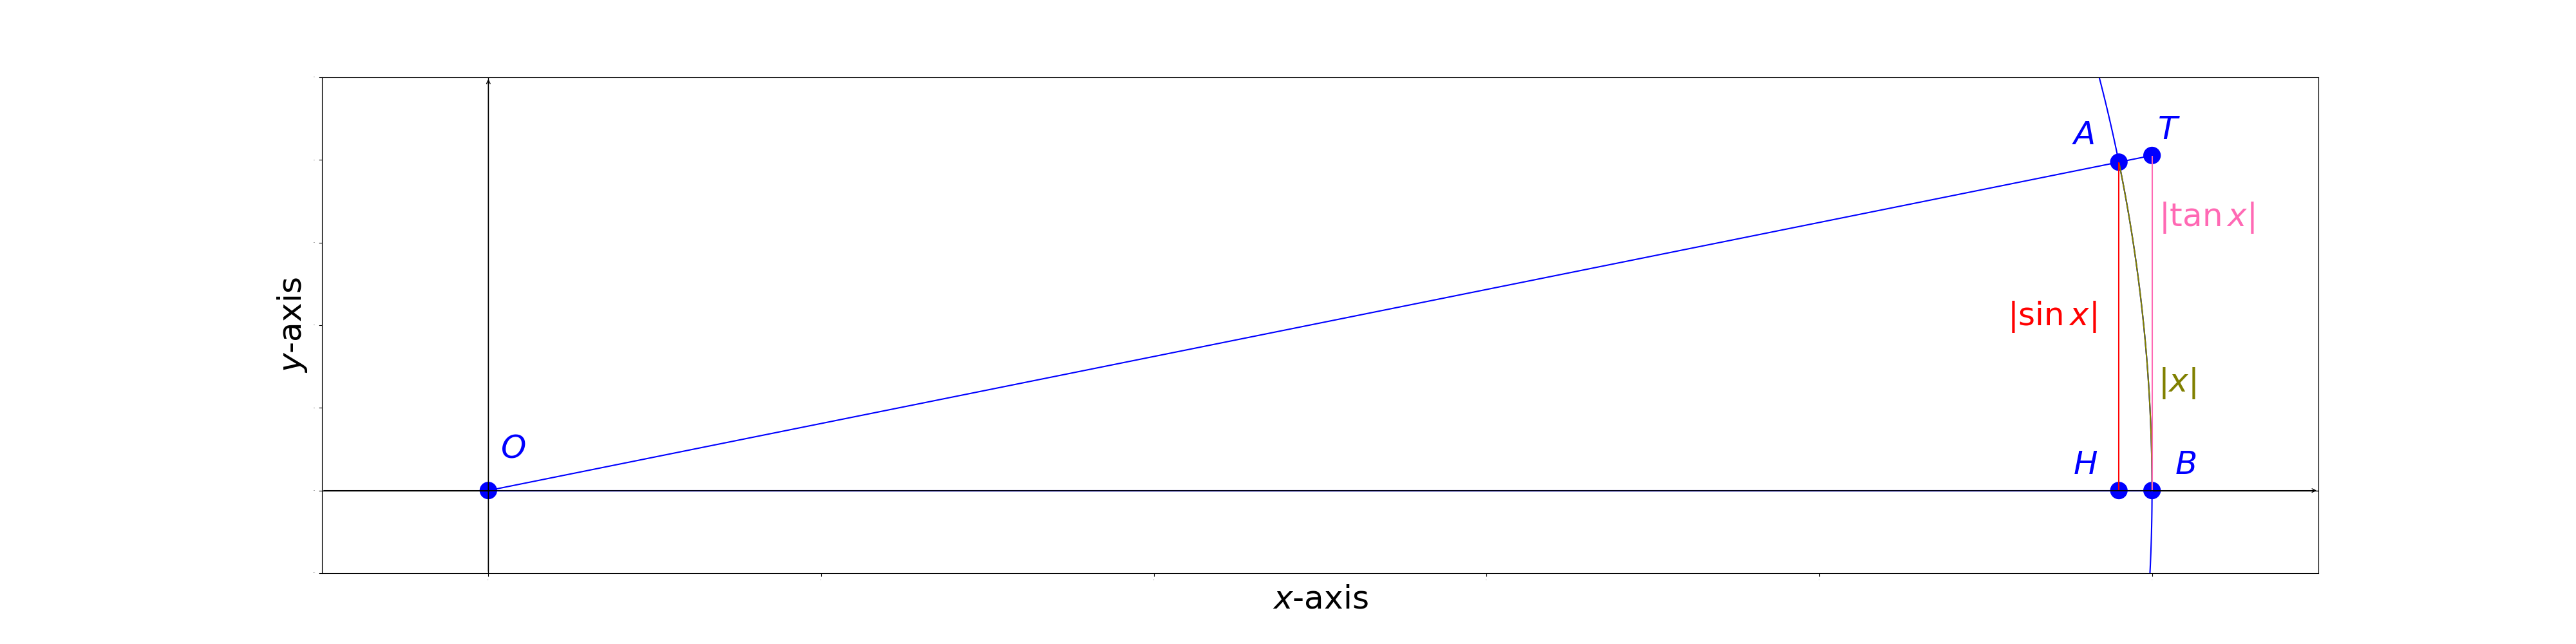
\includegraphics[width=0.79\textwidth]{sandwich_1.png}\figtag{2.3.1}
\end{center}

\begin{example}
    From the last example, we can have $\displaystyle\lim_{x\to 0}\cos x=1$ since $\cos x=\sqrt{1-x^2}$ for $x$ near $0$.
\end{example}

\begin{theorem}
    We have three important trigonometric limits.
    \begin{enumerate}
        \item $\displaystyle\lim_{x\to 0}\dfrac{\sin x}{x}=1$.
        \item $\displaystyle\lim_{x\to 0}\dfrac{1-\cos x}{x}=0$.
        \item $\displaystyle\lim_{x\to 0}\dfrac{1-\cos x}{x^2}=\dfrac{1}{2}$.
    \end{enumerate}
\end{theorem}
\textbf{Proof}. We first show that $\displaystyle\lim_{x\to 0}\dfrac{\sin x}{x}=1$. From Figure 2.3.1, we can see that $\Delta TOB$ contains circular sector $AOB$, and circular sector $AOB$ contains $\Delta AOB$. Hence, we have the inequalities about their area, $$\dfrac{1}{2}\cdot1\cdot |\sin x|\leq\dfrac{1}{2}\cdot1\cdot|x|\leq\dfrac{1}{2}\cdot 1\cdot |\tan x|$$ for $|x|\leq\dfrac{\pi}{2}$. Dividing the inqualities by $\dfrac{|\sin x|}{2}$, we have $$1\leq\dfrac{|x|}{|\sin x|}\leq\dfrac{1}{|\cos x|}.$$ Since $\dfrac{x}{\sin x}$ and $\dfrac{1}{\cos x}$ are positive near $0$, we can pill off the absolute values and take reciprocals of them, having $$1\geq\dfrac{\sin x}{x}\geq\cos x.$$ Since $\displaystyle\lim_{x\to 0}1=1$ and $\displaystyle\lim_{x\to 0}\cos x=1$, we have $\displaystyle\lim_{x\to 0}\dfrac{\sin x}{x}=1$ by the sandwich theorem. The second limit follows from the first limit:
\begin{align*}
    \lim_{x\to 0}\dfrac{1-\cos x}{x}&=\lim_{x\to 0}\dfrac{1-\cos x}{x}\cdot\dfrac{1+\cos x}{1+\cos x}\\
    &=\lim_{x\to 0}\dfrac{1^2-(\cos x)^2}{x(1+\cos x)}\\
    &=\lim_{x\to 0}\dfrac{(\sin x)^2}{x(1+\cos x)}\\
    &=\lim_{x\to 0}\dfrac{\sin x}{x}\cdot\dfrac{\sin x}{(1+\cos x)}\\
    &=\lim_{x\to 0}\dfrac{\sin x}{x}\cdot\lim_{x\to 0}\dfrac{\sin x}{(1+\cos x)}\\
    &=1\cdot0\\
    &=0.
\end{align*} The third limit also follows from the first limit: 

\begin{align*}
    \lim_{x\to 0}\dfrac{1-\cos x}{x^2}&=\lim_{x\to 0}\dfrac{1-\cos x}{x^2}\cdot\dfrac{1+\cos x}{1+\cos x}\\
    &=\lim_{x\to 0}\dfrac{(\sin x)^2}{x^2(1+\cos x)}\\
    &=\lim_{x\to 0}\dfrac{(\sin x)^2}{x^2}\cdot\dfrac{1}{(1+\cos x)}\\
    &=\lim_{x\to 0}\dfrac{(\sin x)^2}{x^2}\cdot\lim_{x\to 0}\dfrac{1}{(1+\cos x)}\\
    &=1^2\cdot\dfrac{1}{2}\\
    &=\dfrac{1}{2}.
\end{align*} \qed

\begin{example}
    Evaluate the following limits.
    \begin{enumerate}
        \item $\displaystyle\lim_{x\to 0}\dfrac{\sin 2x}{5x}$.
        \item $\displaystyle\lim_{x\to 0}x\cot7x$.
    \end{enumerate}
\end{example}
\textbf{Solution}. For the first limit, we set $h=2x$. Then, the limit becomes \begin{align*}
    \lim_{h\to 0}\dfrac{2}{5}\cdot\dfrac{\sin h}{h}&=\dfrac{2}{5}\cdot\lim_{h\to 0}\dfrac{\sin h}{h}\\
    &=\dfrac{2}{5}\cdot1\\
    &=\dfrac{2}{5}.
\end{align*} For the second limit, we set $t=7x$. Then, the limit becomes \begin{align*}
    \lim_{t\to 0}\dfrac{1}{7}\cdot\dfrac{t\cos t}{\sin t}&=\dfrac{1}{7}\cdot\lim_{t\to 0}\cos t\cdot\dfrac{t}{\sin t}\\
    &=\dfrac{1}{7}\cdot\lim_{t\to 0}\cos t\cdot\lim_{t\to 0}\dfrac{t}{\sin t}\\
    &=\dfrac{1}{7}\cdot1\cdot1\\
    &=\dfrac{1}{7}.
\end{align*} \qed

We now define an essential number for our future studies.

\begin{definition}[Euler's Number]
    Let $r\in\bbR$. If $\displaystyle\lim_{h\to 0}\dfrac{r^h-1}{h}=1$, then the number $r$ is called \underline{Euler's number} and is denoted $e$. This number is uniquely defined and has at least three kinds of equivalent definitions. The exponential function is defined with base $e$.
\end{definition}

\subsection*{Exercise}

\begin{enumerate}[label=\arabic*.]
    \item Suppose $\displaystyle\lim_{x\to c}f(x)=4$, $\displaystyle\lim_{x\to c}g(x)=-4$. Evaluate the following limits if one exists. Otherwise, explain the reason that one does not exist.
    \begin{enumerate}
        \begin{multicols}{4}
            \item $\displaystyle\lim_{x\to c}f(x)+g(x)$.
            \item $\displaystyle\lim_{x\to c}f(x)-g(x)$.
            \item $\displaystyle\lim_{x\to c}f(x)g(x)$.
            \item $\displaystyle\lim_{x\to c}f(x)/g(x)$.
        \end{multicols}
    \end{enumerate}
    \item Suppose $\displaystyle\lim_{x\to c}f(x)=2$, $\displaystyle\lim_{x\to c}g(x)=-1$, and $\displaystyle\lim_{x\to c}h(x)=0$. Evaluate the following limits if one exists. Otherwise, explain the reason that one does not exist.
    \begin{enumerate}
        \begin{multicols}{3}
            \item $\displaystyle\lim_{x\to c}\dfrac{2f(x)+g(x)}{2}$.
            \item $\displaystyle\lim_{x\to c}\dfrac{1}{f(x)+2g(x)}$.
            \item $\displaystyle\lim_{x\to c}\dfrac{f(x)}{g(x)}$.
            \item $\displaystyle\lim_{x\to c}\dfrac{h(x)}{f(x)}$.
            \item $\displaystyle\lim_{x\to c}\dfrac{f(x)}{h(x)}$.
            \item $\displaystyle\lim_{x\to c}\dfrac{1}{f(x)-g(x)}$.
        \end{multicols}
    \end{enumerate}
    \item Suppose $\displaystyle\lim_{x\to c}f(x)=3$, $\displaystyle\lim_{x\to c}g(x)=0$, and $\displaystyle\lim_{x\to c}h(x)=-2$. Evaluate the following limits if one exists. Otherwise, explain the reason that one does not exist.
    \begin{enumerate}
        \begin{multicols}{3}
            \item $\displaystyle\lim_{x\to c}\dfrac{2f(x)-2h(x)}{g(x)}$.
            \item $\displaystyle\lim_{x\to c}\dfrac{g(x)(h(x))^3}{f(x)}$.
            \item $\displaystyle\lim_{x\to c}\dfrac{f(x)}{x-c}$.
            \item $\displaystyle\lim_{x\to c}\dfrac{g(x)}{h(x)}$.
            \item $\displaystyle\lim_{x\to c}\dfrac{1}{f(x)-h(x)}$.
            \item $\displaystyle\lim_{x\to c}(3+g(x))^2$.
        \end{multicols}
    \end{enumerate}
    \item Evaluate the following limits if one exists. Otherwise, explain the reason that one does not exist.
    \begin{enumerate}
        \begin{multicols}{4}
            \item $\displaystyle\lim_{x\to 2}3$.
            \item $\displaystyle\lim_{x\to 3}(5-4x)^2$.
            \item $\displaystyle\lim_{x\to -4}x^2+3x-7$.
            \item $\displaystyle\lim_{x\to -2}3|x-1|$.
        \end{multicols}
    \end{enumerate}
    \item Evaluate the following limits if one exists. Otherwise, explain the reason that one does not exist.
    \setlength{\delimitershortfall}{0pt}
    \begin{enumerate}
        \begin{multicols}{3}
            \item $\displaystyle\lim_{x\to 0}\dfrac{x^2-1}{x-1}$.
            \item $\displaystyle\lim_{x\to 3}\dfrac{x^2+x-12}{x-3}$.
            \item $\displaystyle\lim_{x\to 4}\left(\dfrac{1}{x}-\dfrac{1}{4}\right)\left(\dfrac{1}{x-4}\right)$.
            \item $\displaystyle\lim_{h\to 0}h\cdot\left(1-\dfrac{1}{h}\right)$.
            \item $\displaystyle\lim_{x\to 1}\dfrac{x-1}{\sqrt{x}-1}$.
            \item $\displaystyle\lim_{x\to 4}\dfrac{\sqrt{x}-2}{x-4}$.
            \item $\displaystyle\lim_{x\to 0}\dfrac{\sqrt{x^2-4}}{x-2}$.
            \item $\displaystyle\lim_{t\to 0}\dfrac{t+a/t}{t+b/t}$.
            \item $\displaystyle\lim_{h\to 0}h^2\left(1+\dfrac{1}{h}\right)$.
            \item $\displaystyle\lim_{h\to 0}h\left(1+\dfrac{1}{h^2}\right)$.
            \item $\displaystyle\lim_{x\to -4}\dfrac{2x}{x+4}+\dfrac{8}{x+4}$.
            \item $\displaystyle\lim_{x\to -4}\dfrac{2x}{x+4}-\dfrac{8}{x+4}$.
        \end{multicols}
    \end{enumerate}
    \item Evaluate the following limits if one exists. Otherwise, explain the reason that one does not exist.
    \begin{enumerate}
        \begin{multicols}{2}
            \item $\displaystyle\lim_{x\to 4}\dfrac{1}{x}-\dfrac{1}{4}$.
            \item $\displaystyle\lim_{x\to 4}\left(\dfrac{1}{x}-\dfrac{1}{4}\right)\left(\dfrac{1}{x-4}\right)$.
            \item $\displaystyle\lim_{x\to 4}\left(\dfrac{1}{x}-\dfrac{1}{4}\right)\left(x-2\right)$.
            \item $\displaystyle\lim_{x\to 4}\left(\dfrac{1}{x}-\dfrac{1}{4}\right)\left(\dfrac{1}{x-4}\right)^2$.
        \end{multicols}
    \end{enumerate}
    \item Evaluate the following limits if one exists. Otherwise, explain the reason that one does not exist.
    \begin{enumerate}
        \begin{multicols}{2}
            \item $\displaystyle\lim_{x\to 0}\dfrac{\sin 3x}{x}$.
            \item $\displaystyle\lim_{x\to 0}\dfrac{\sin 2x}{5x}$.
            \item $\displaystyle\lim_{x\to 0}\dfrac{3x}{\sin 4x}$.
            \item $\displaystyle\lim_{x\to 0}\dfrac{\sin (x^2)}{x^2}$.
            \item $\displaystyle\lim_{x\to 0}\dfrac{(\sin 2x)^2}{(5x)^2}$.
            \item $\displaystyle\lim_{x\to 0}x\csc x$.
            \item $\displaystyle\lim_{x\to 0}\dfrac{x^2}{1-\cos 2x}$.
            \item $\displaystyle\lim_{x\to 0}\dfrac{4 x^2}{\cot (3x^2)}$.
            \item $\displaystyle\lim_{x\to 0}\dfrac{1-\cos 4x}{9x^2}$.
            \item $\displaystyle\lim_{x\to\pi}\dfrac{\sin x}{x-\pi}$.
            \item $\displaystyle\lim_{x\to 0}\dfrac{\sin ax}{x}, \quad a\ne0$.
            \item $\displaystyle\lim_{x\to 0}\dfrac{\sin x}{bx}, \quad b\ne0$.
            \item $\displaystyle\lim_{x\to 0}\dfrac{\sin ax}{bx}, \quad a\ne0, \ \ b\ne0$.
            \item $\displaystyle\lim_{x\to 0}\dfrac{\sin ax}{\sin bx}, \quad a\ne0, \ \ b\ne0$.
            \item $\displaystyle\lim_{x\to 0}\dfrac{\cos ax}{\cos bx}, \quad a\ne0, \ \ b\ne0$.
            \item $\displaystyle\lim_{x\to 0}\dfrac{\tan ax}{\tan bx}, \quad a\ne0, \ \ b\ne0$.
        \end{multicols}
    \end{enumerate}
    \item Find the value of $r$ for each of the following constrain.
    \begin{enumerate}
        \begin{multicols}{2}
            \item $\displaystyle\lim_{x\to 0}\dfrac{\sin (rx)}{2x}=4$.
            \item $\displaystyle\lim_{x\to 0}\dfrac{1-\cos (rx)}{x^2}=1$.
            \item $\displaystyle\lim_{x\to 0}\dfrac{e^{rx}-1}{x}=2$.
            \item $\displaystyle\lim_{x\to 0}\dfrac{e^{5x}-1}{rx}=1$.
        \end{multicols}
    \end{enumerate}
    \item Show that the each of the following statements hold.
        \begin{enumerate}
            \item $\displaystyle\lim_{x\to 0}x\sin\left(\dfrac{1}{x}\right)=0$.
            \setlength{\delimitershortfall}{13.5pt}
            \item $\displaystyle\lim_{x\to 0}x\cdot f(x)=0$, where $f(x)=\left\{\begin{array}{rl}
                1,\quad & \text{if $x\in\mathbb{Q}$},\\
                -1,\quad & \text{if $x\notin\mathbb{Q}$}.
            \end{array}\right.$
            \setlength{\delimitershortfall}{0pt}
        \end{enumerate}
    \setlength{\delimitershortfall}{13.5pt}
\end{enumerate}

\section{Continuity}

As we discussed in the last section, the meaning of continuous is that the value of the function is the limit.

\begin{definition}[Continuous]
    Let $f:A\to\bbR$ be a function, where $A\subseteq\bbR$. Let $c\in A$. We say that $f$ is \underline{continuous} at $c$ if $\displaystyle\lim_{x\to c}f(x)=f(c)$.
\end{definition}

After defining continuity at a point, we can define continuity on a set and continuous function.

\begin{definition}[Continuous]
    Let $f:A\to\bbR$ be a function, where $A\subseteq\bbR$. Let $C\subseteq A$. We say that $f$ is \underline{continuous} on $C$ if $\displaystyle\lim_{x\to c}f(x)=f(c)$ for all $c\in C$.
\end{definition}

\begin{definition}[Continuous]
    Let $f:A\to\bbR$ be a function, where $A\subseteq\bbR$. We say that $f$ is \underline{continuous} if $\displaystyle\lim_{x\to c}f(x)=f(c)$ for all $c\in A$.
\end{definition}

Using Theorem \ref{lim_op}, we have the following theorem.

\begin{theorem}[Operations for Continuous Functions]\label{conti_op}
    Let $f, g$ be two functions. If $f$ and $g$ are continuous at $c$, the following statements hold.
    \begin{enumerate}
        \item $f+g$ is continuous at $c$.
        \item $\alpha f$ is continuous at $c$, where $\alpha\in\bbR$.
        \item $fg$ is continuous at $c$.
        \item If $g(c)\ne0$, then $\dfrac{f}{g}$ is continuous at $c$.
    \end{enumerate}
\end{theorem}

We also have a theorem about composite functions.

\begin{theorem}
    Let $f, g$ be two functions. If $g$ is continuous at $c$ and $f$ is continuous at $g(c)$, then $f\circ g$ is continuous at $c$.
\end{theorem}

\begin{example} 
    The function $f(x)=\sqrt{\dfrac{x^2+1}{x-3}}$ is continuous on $(3, \infty)$. The function $f$ can be decomposed by $f_1\circ f_2$, where \begin{equation*}
        f_1(x)=\sqrt{x},\quad f_2(x)=\dfrac{x^2+1}{x-3}.
    \end{equation*}
\end{example}

\begin{example} 
    The function $f(x)=\dfrac{1}{5-\sqrt{x^2+16}}$ is a continuous function since it is continuous everywhere except at $\pm3$, which is not defined. The function $f$ can be decomposed by $f_1\circ f_2\circ f_3\circ f_4$, where \begin{equation*}
        f_1(x)=\dfrac{1}{x}, \quad f_2(x)=5-x, \quad f_3(x)=\sqrt{x}, \quad f_4(x)=x^2+16.
    \end{equation*}
\end{example}

We can also define one-sided continuity just as one-sided limits.

\begin{definition}[Left Continuity]
    Let $f:A\to\bbR$ be a function, where $A\subseteq\bbR$. Let $c\in A$. We say that $f$ is \underline{continuous from the left} at $c$ if $\displaystyle\lim_{x\to c^-}f(x)=f(c)$.
\end{definition}

\begin{definition}[Right Continuity]
    Let $f:A\to\bbR$ be a function, where $A\subseteq\bbR$. Let $c\in A$. We say that $f$ is \underline{continuous from the right} at $c$ if $\displaystyle\lim_{x\to c^+}f(x)=f(c)$.
\end{definition}

\begin{theorem}
    A function $f$ is continuous at $c$ if and only if all $f(c)$, $\displaystyle\lim_{x\to c^-}f(x)$, and $\displaystyle\lim_{x\to c^+}f(x)$ exist and are equal.
\end{theorem}

\begin{example}
    Determine the discontinuities, if any, of the following function $$f(x)=\left\{\begin{array}{rl}
        2x+1,\quad & \text{if $x\leq 0$},\\
        1, \quad & \text{if $0\leq x\leq 1$},\\
        x^2+1, \quad & \text{if $x>1$}.
    \end{array}\right.$$
\end{example}
\textbf{Solution}. Clearly, $f$ is continuous on $(-\infty, 0)$, on $(0, 1)$, and on $(1, \infty)$. We check whether $f$ is continuous at $0$ and at $1$. The left-hand-side limit of $f$ at $0$ is $$\lim_{x\to 0^-}2x+1=1$$ amd the right-hand-side limit of $f$ at $0$ is $$\lim_{x\to 0^+}1=1.$$ Hence, $f$ is continuous at $0$. The left-hand-side limit of $f$ at $1$ is $$\lim_{x\to 1^-}1=1$$ amd the right-hand-side limit of $f$ at $1$ is $$\lim_{x\to 1^+}x^2+1=2.$$ Hence, $f$ is not continuous at $0$. Therefore, $x=1$ is the only discontinuity. \qed

Different discontinuities yields different scenarios: some lost a point, some is shifted for a certain amount, and some goes to infinity or minus infinity. We can classity discontinuities with three different genres.

\begin{definition}[Removable Discontinuity]
    Let $f$ be a function. Suppose $f$ is not continuous at $c$. We say the discontinuity is a \underline{removable discontinuity} if we can redefine $f(c)$ such that $f$ is continuous at $c$.
\end{definition}

\begin{definition}[Jump Discontinuity]
    Let $f$ be a function. Suppose $f$ is not continuous at $c$. We say the discontinuity is a \underline{jump discontinuity} if $\displaystyle\lim_{x\to c^-}f(x)\ne\lim_{x\to c^+}f(x)$.
\end{definition}

\begin{definition}[Essential Discontinuity]
    Let $f$ be a function. Suppose $f$ is not continuous at $c$. We say the discontinuity is an \underline{essential discontinuity} if $\displaystyle\lim_{x\to c^-}f(x)$ does not exist or $\displaystyle\lim_{x\to c^+}f(x)$ does not exist.
\end{definition}

\begin{example}
    In Figure 2.4.1, $f$ has a jump discontinuity at $2$, a removable discontinuity at $6$, and a critical discontinuity at $8$.
\end{example}
\textbf{Proof}. The two one-sided limits of $f$ at $2$ are different; we can define $f(6)=1$ to make $f$ continuous at $6$. The value of $f$ gets larger and larger as $x$ approaches $8$ from the left; hence $f$ is unbounded near $8$. \qed 

If a function $f$ is continuous on an interval $I$, there will be neither holes nor jumps for the graph of $f$ on $I$. We can describe this by the intermediate value theorem. This theorem garuantees that every value between values of endpoints will be attained on the interval where $f$ is continuous.

\begin{center}
    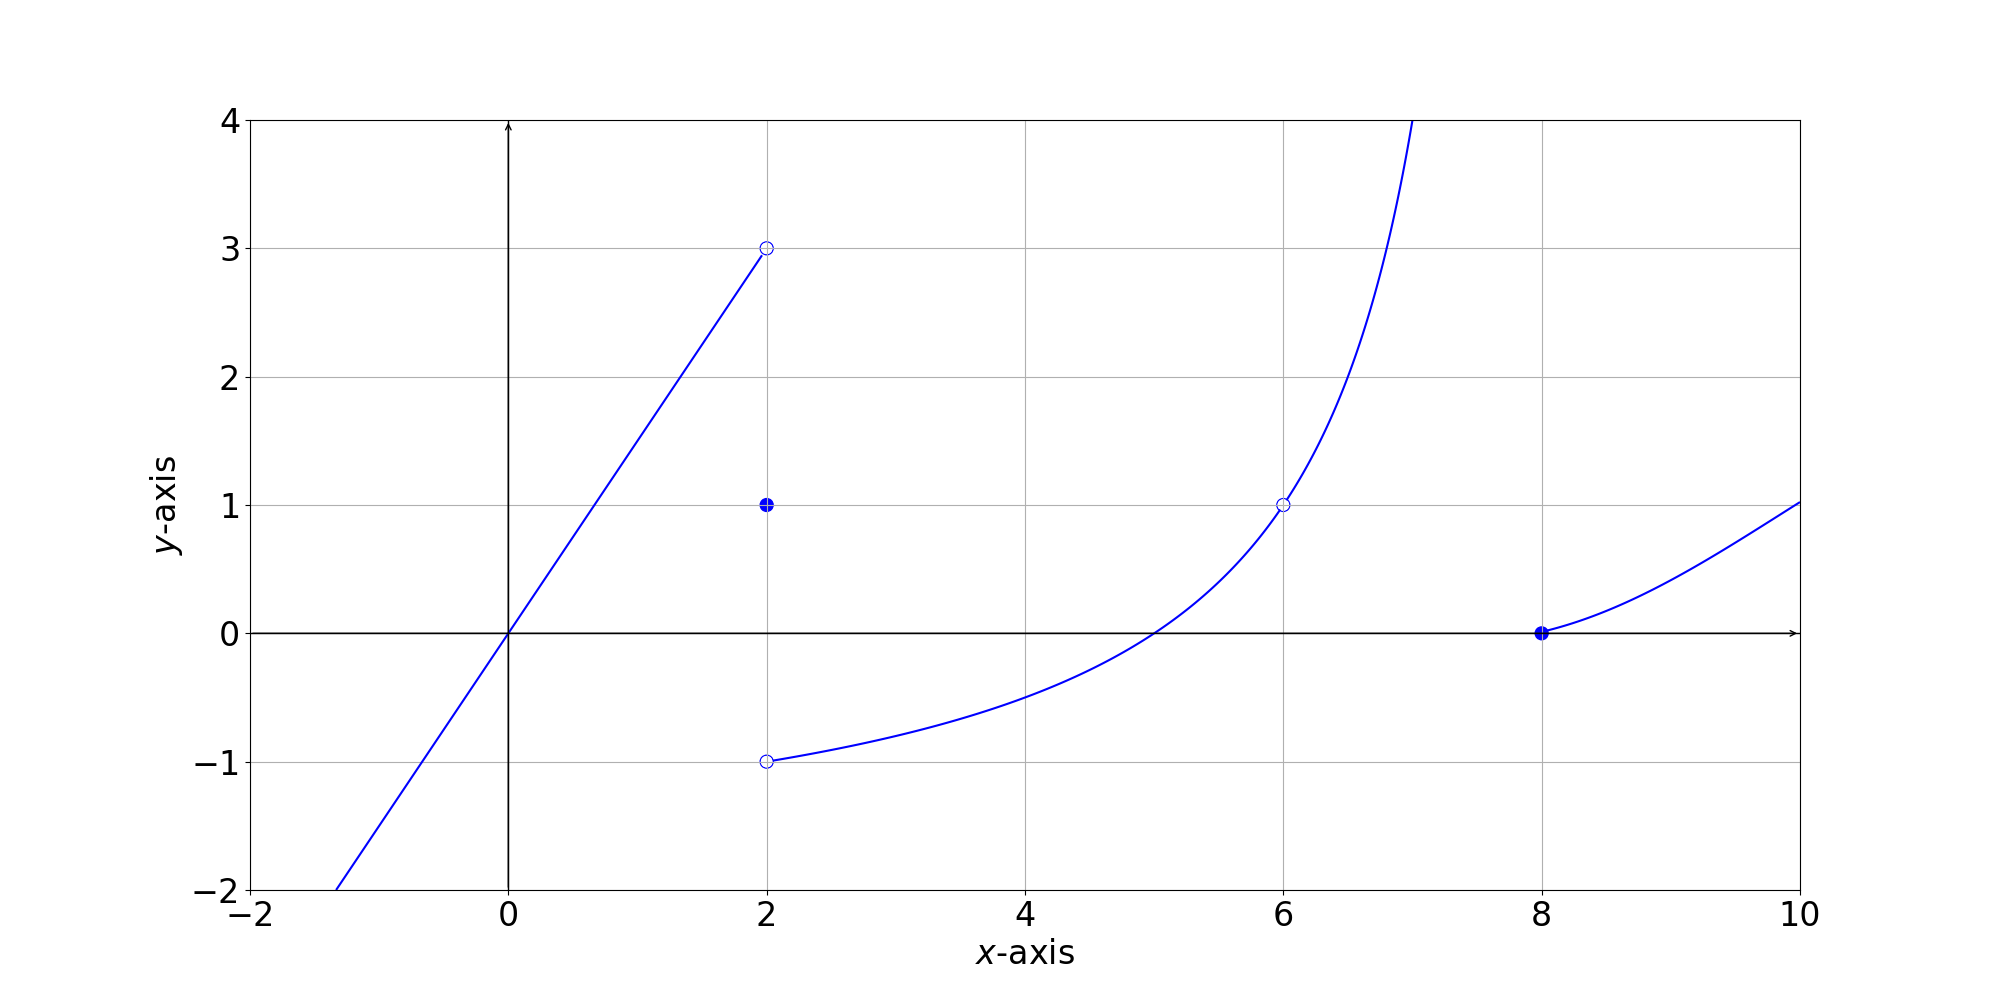
\includegraphics[width=0.95\textwidth]{discontinuity.png}\figtag{2.4.1}
\end{center}

\begin{theorem}[Intermediate Value Theorem]
    If $f$ is continuous on a closed interval $[a, b]$ (this interval is set to be bounded as $a, b\in\bbR$) and $y_0$ is an arbitrary number between $f(a)$ and $f(b)$, then there is a number $c\in(a, b)$ such that $f(c)=y_0$.
\end{theorem}

\begin{example}
    Let $f(x)=x^2-2$. Then, $f(1)=-1$ and $f(2)=2$. Hence, by the intermediate value theorem, there is a number $c\in(1, 2)$ such that $f(c)=0$, i.e., $c^2=2$. The number $c$ is unique, and it is called $\sqrt{2}$.
\end{example}

\begin{example}
    Let $f$ be continuous on $[0, 2]$. Suppose $f(0)=-2$ and $f(2)=7$. Then, there is a number $c\in(0, 2)$ such that $f(c)=0$, i.e., $c$ is a root of $f$.
\end{example}

From the intermediate value theorem, we know that a continuous function maps an interval to another interval. If the interval of domain is closed and bounded (the values in it are finite), then a maximum and a minimum will be granted by the extreme value theroem.

\begin{theorem}[Extreme Value Theorem]
    If $f$ is continuous on a closed interval $[a, b]$, then there is a number $c_1\in[a, b]$ such that $\displaystyle f(c_1)=\max_{x\in[a, b]}f(x)$ and $\displaystyle f(c_2)=\min_{x\in[a, b]}f(x)$.
\end{theorem}

\begin{example}
    In Figure 2.4.2, this function attains neither a maximum nor a minimum on $[0, 2]$ since it is not continuous on the endpoints.
\end{example}

From the extreme value theorem, we know that a continuous function maps a closed and bounded interval to another closed and bounded interval.

\begin{remark}
    One have to check the interval of continuity, then apply the intermediate value theorem or the extreme value theroem.
\end{remark}

\begin{center}
    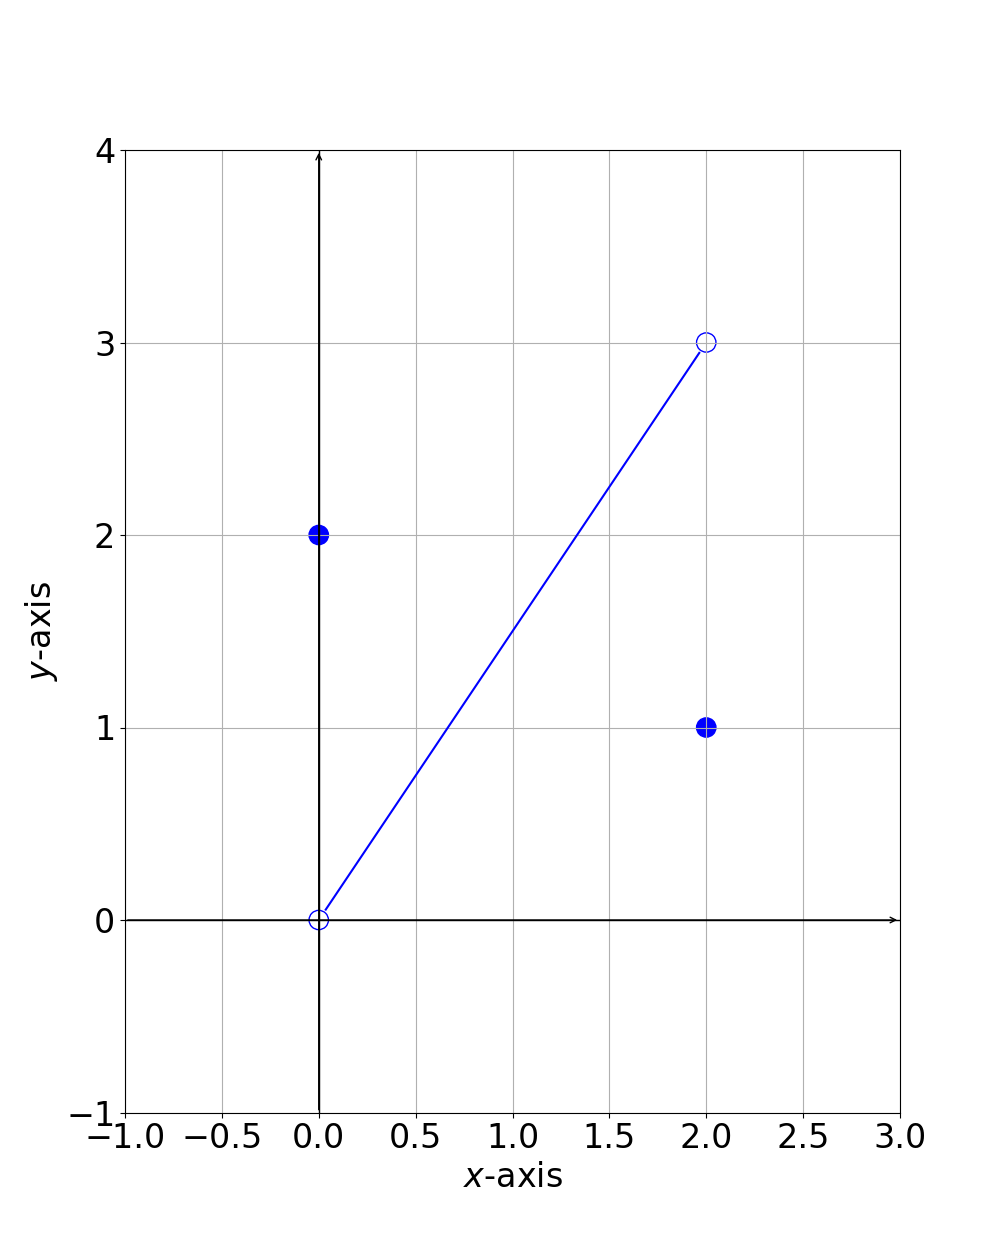
\includegraphics[width=0.45\textwidth]{evt.png}\figtag{2.4.2}
\end{center}


\subsection*{Exercise}

\begin{enumerate}[label=\arabic*.]
    \item Determine points such that $f$ is discontinuous at. Determine the genre of each discontinuity. Determine whether $f$ is continuous from the right, from the left, or neither for each discontinuity.
    \begin{center}
        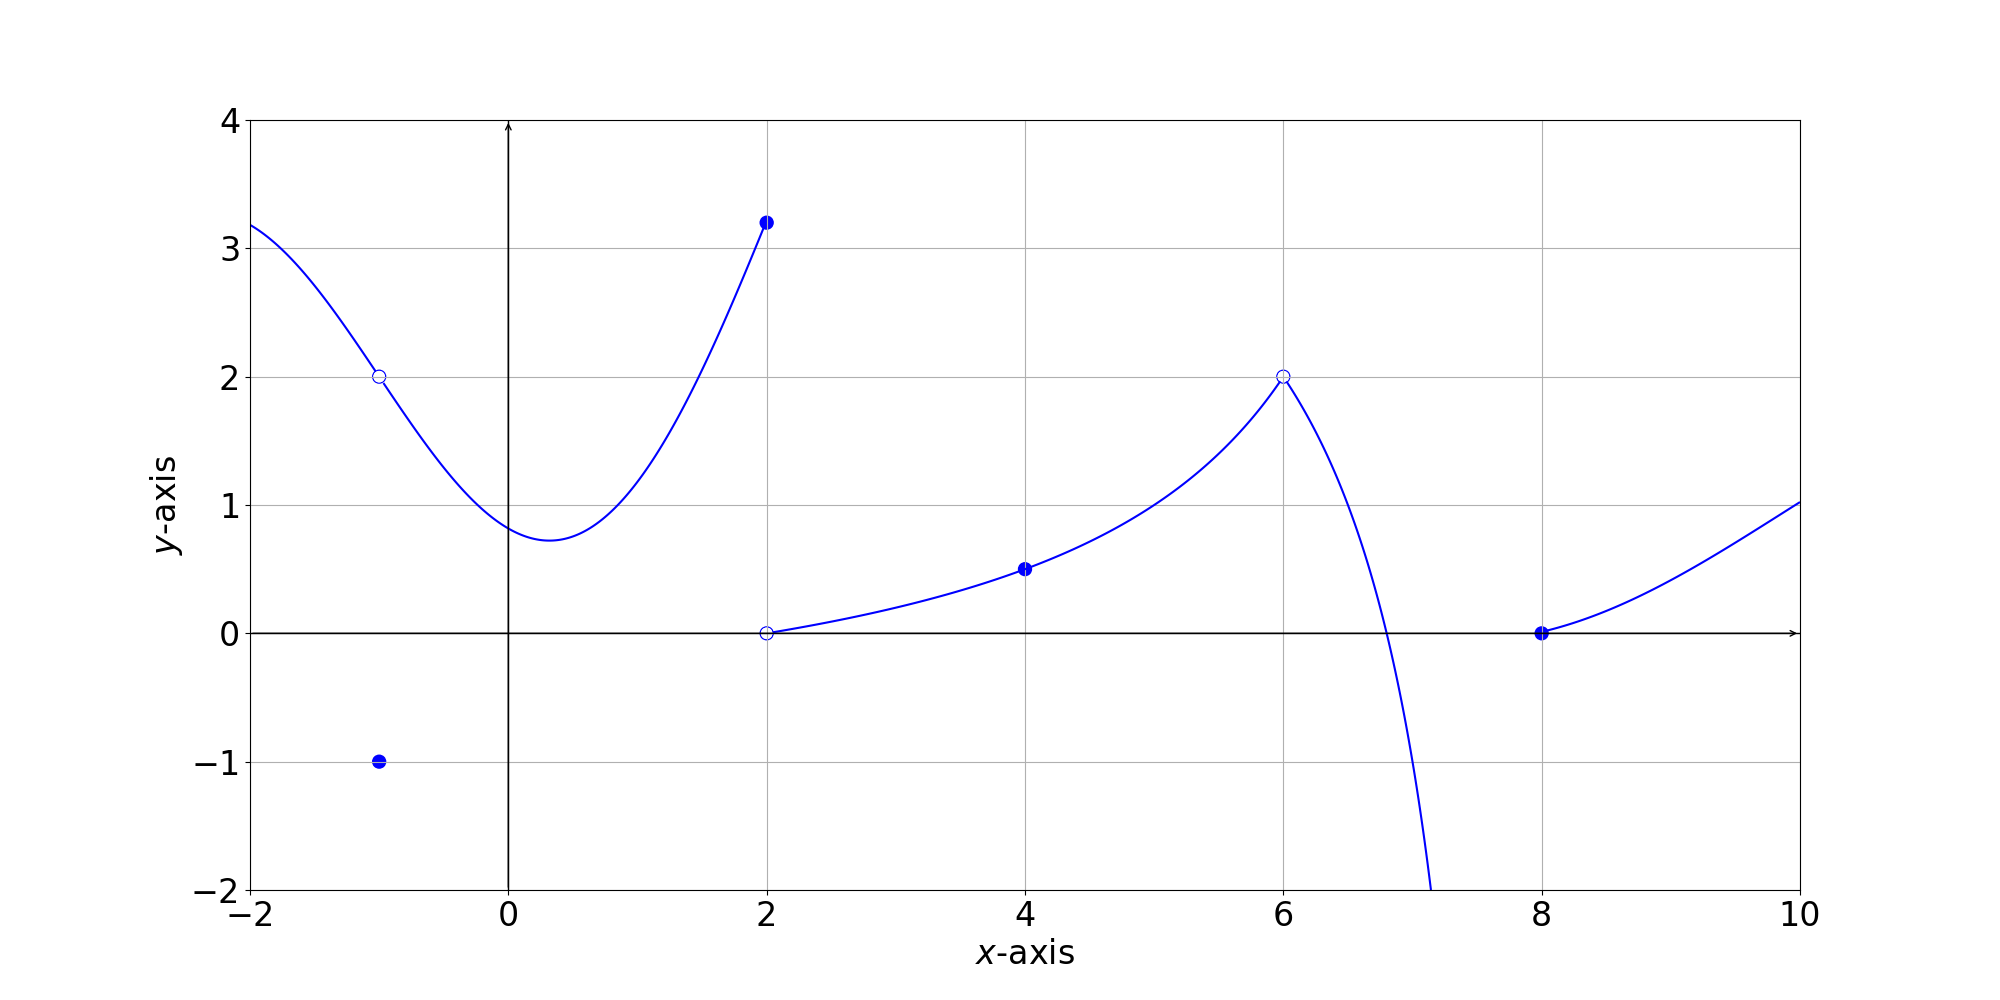
\includegraphics[width=0.87\textwidth]{continuity_exercise_1.png}
    \end{center}
    \item Determine whether the function is continuous at the indicated point. If not, determine the genre of each discontinuity.
    \begin{enumerate}
        \begin{multicols}{2}
            \item $f(x)=x^3-5x+1,\quad x=2$.
            \item $f(x)=\sqrt{(x-3)^2+9},\quad x=3$.
            \item $f(x)=\sqrt{x^2+4}, \quad x=-2$.
            \item $f(x)=|x-7|,\quad x=7$.
        \end{multicols}
    \end{enumerate}
    \item Determine whether the function is continuous at the indicated point. If not, determine the genre of each discontinuity.
    \begin{enumerate}
        \begin{multicols}{2}
            \item $f(x)=\left\{\begin{array}{rl}
                x^2+4, \quad & \text{if $x<2$},\\
                8, \quad & \text{if $x=2$},\\
                x^3, \quad & \text{if $x>2$},
            \end{array}\right., \quad x=2$.
            \item $f(x)=\left\{\begin{array}{rl}
                x^2+5, \quad & \text{if $x<2$},\\
                x^3, \quad & \text{if $x\geq 2$},
            \end{array}\right., \quad x=2$.
            \item $f(x)=\left\{\begin{array}{rl}
                x^2+4, \quad & \text{if $x<2$},\\
                5, \quad & \text{if $x=2$},\\
                x^3, \quad & \text{if $x>2$},
            \end{array}\right., \quad x=2$.
            \item $f(x)=\left\{\begin{array}{rl}
                x^2+5, \quad & \text{if $x<2$},\\
                10, \quad & \text{if $x=2$},\\
                x^3+1, \quad & \text{if $x>2$},
            \end{array}\right., \quad x=2$.
            \item $f(x)=\left\{\begin{array}{rl}
                \dfrac{|x-1|}{x-1}, \quad & \text{if $x\ne1$},\\
                0, \quad & \text{if $x=1$},
            \end{array}\right., \quad x=1$.
            \item $f(x)=\left\{\begin{array}{rl}
                1-x, \quad & \text{if $x<1$},\\
                1, \quad & \text{if $x=1$},\\
                x^3-1, \quad & \text{if $x>1$},
            \end{array}\right., \quad x=1$.
        \end{multicols}
    \end{enumerate}
    \item If possible, redefine the function at $1$ so that $f$ is continuous at $1$. Otherwise, explain the reason that $f$ cannot be continuous with any redefinition.
    \begin{enumerate}
        \begin{multicols}{2}
            \item $f(x)=\dfrac{x^2-1}{x-1}$.
            \item $f(x)=\dfrac{x-1}{|x-1|}$.
            \item $f(x)=\dfrac{(x-1)^2}{|x-1|}$.
            \item $f(x)=\dfrac{1}{x-1}$.
        \end{multicols}
    \end{enumerate}
    \item If possible, redefine the function at $0$ so that $f$ is continuous at $0$. Otherwise, explain the reason that $f$ cannot be continuous with any redefinition.
    \begin{enumerate}
        \begin{multicols}{2}
            \item $f(x)=\dfrac{\sin 5x}{\sin 3x}$.
            \item $f(x)=\dfrac{x^2}{\cos 4x-1}$.
            \item $f(x)=\dfrac{\sin x}{|x|}$.
            \item $f(x)=\dfrac{x\sin2x}{\sin(x^2)}$.
        \end{multicols}
    \end{enumerate}
    \item If possible, redefine the function at $5$ so that $f$ is continuous at $5$. Otherwise, explain the reason that $f$ cannot be continuous with any redefinition.
    \begin{enumerate}
        \begin{multicols}{2}
            \item $f(x)=\dfrac{\sqrt{x+4}-3}{x-5}$.
            \item $f(x)=\dfrac{\sqrt{x+4}-3}{\sqrt{x-5}}$.
            \item $f(x)=\dfrac{\sqrt{2x-1}-3}{x-5}$.
            \item $f(x)=\dfrac{\sqrt{x^2-7x+16}-\sqrt{6}}{(x-5)\sqrt{x+1}}$.
        \end{multicols}
    \end{enumerate}
    \item What is the value of $A$ so that the function $$f(x)=\left\{\begin{array}{rl}
        x^2, \quad & \text{if $x<1$},\\
        Ax-3, \quad & \text{if $x\geq1$}
    \end{array}\right.$$ is continuous at $1$?
    \item What is the value of $A$ so that the function $$f(x)=\left\{\begin{array}{rl}
        A^2x^2, \quad & \text{if $x\leq2$},\\
        (1-A)x, \quad & \text{if $x>2$}
    \end{array}\right.$$ is continuous at $2$?
    \item What are the values of $A$ and $B$ so that the function $$f(x)=\left\{\begin{array}{rl}
        2x^2-1, \quad & \text{if $x<2$},\\
        A \quad &\text{if $x=2$},\\
        x^3-2Bx, \quad & \text{if $x>2$}
    \end{array}\right.$$ is continuous at $2$?
    \item What is the value of $A$ so that the function $$f(x)=\left\{\begin{array}{rl}
        1+Ax, \quad & \text{if $x<2$},\\
        A-x, \quad & \text{if $x\geq2$}
    \end{array}\right.$$ is continuous at $2$? Is $f$ continuous on $\bbR$?
    \item Use the intermediate value theorem to show that there is a solution to the given equation in the given interval. 
    \begin{enumerate} \setlength{\delimitershortfall}{0pt}
        \item $2x^3-4x^2+5x-4=0, \quad [1, 2]$.
        \item $x^4-x+1=0, \quad [-1, 1]$.
        \item $\sin x+2\cos x-x^2=0, \quad \left[0, \dfrac{\pi}{2}\right]$.
        \item $2\tan x-x=1,\quad \left[0, \dfrac{\pi}{4}\right]$.
    \end{enumerate} \setlength{\delimitershortfall}{13.5pt}
    \item Show that there is a number $c\in\bbR$ such that $c^3-2c^2-1=6$.
    \item Sketch the graph of a function $f$ on $[0, 1]$, which meets the given conditions, if possible. Otherwise, explain the reason that you cannot do so.
    \begin{enumerate}
        \item $f$ is continuous on $[0, 1]$ with minimum $0$ and maximum $1$.
        \item $f$ is continuous on $[0, 1)$ with minimum $0$ and no maximum.
        \item $f$ is continuous on $[0, 1]$ with minimum $1$ and minimum $0$.
        \item $f$ is continuous on $(0, 1)$ and takes only two distinct values.
        \item $f$ is continuous on $(0, 1)$ and takes only three distinct values.
        \item $f$ is continuous on $(0, 1)$ and is unbounded.
    \end{enumerate}
    \item Locate a root for the following functions with an interval.
    \begin{enumerate}
        \begin{multicols}{2}
            \item $f(x)=x^3+4x-4$.
            \item $f(x)=2x^3-5x+7$.
            \item $f(x)=x^5-3x+1$.
            \item $f(x)=2x^3-\sin x+1$.
        \end{multicols}
    \end{enumerate}
\end{enumerate}

% Formulae for derivatives
\chapter{Derivative and Differentiation}

We started from limits in the world of calculus. We will encounter the two main applications of limits, differentiation and integration, in this chapter and in Chapter 5. Differentiation origins from the problem of looking for a tangent line for a function at a point.

\section{Derivative}

A derivative of $f$ at $c$ is the slope of the tangent line of $f$ at $c$. For example, in Figure 3.1.1, neither lines in pink, in red, nor in olive. They are all secant lines. However, these secant lines $\overleftrightarrow{AP_1}$, $\overleftrightarrow{AP_2}$, and $\overleftrightarrow{AP_3}$ have a tendency to become the tangent line of $f$ at point $A$ as the index of $P$ gets larger. The slope $m_i$ of these lines can be written in a systemetic way: $$m_i=\text{the slope of $\overleftrightarrow{AP_i}$}=\dfrac{y_{P_i}-y_{A}}{x_{P_i}-x_{A}},$$ where $A=(x_A, y_A)$ and $P_i=(x_{P_i}, y_{P_i})$. To describe in texts, the slope is the ratio of the change in $y$ to the change in $x$. This constructs the difference quotient $$\dfrac{f(x+h)-f(x)}{h},$$ which is the slope of a secant line of $f$ through point $(x, f(x))$ and $(x+h, f(x+h))$; note that $f(x+h)-f(x)$ is analygous to $y_{P_i}-y_{A}$ and that $h=(x+h)-x$ is analygous to $x_{P_i}-x_{A}$.

\begin{center}
    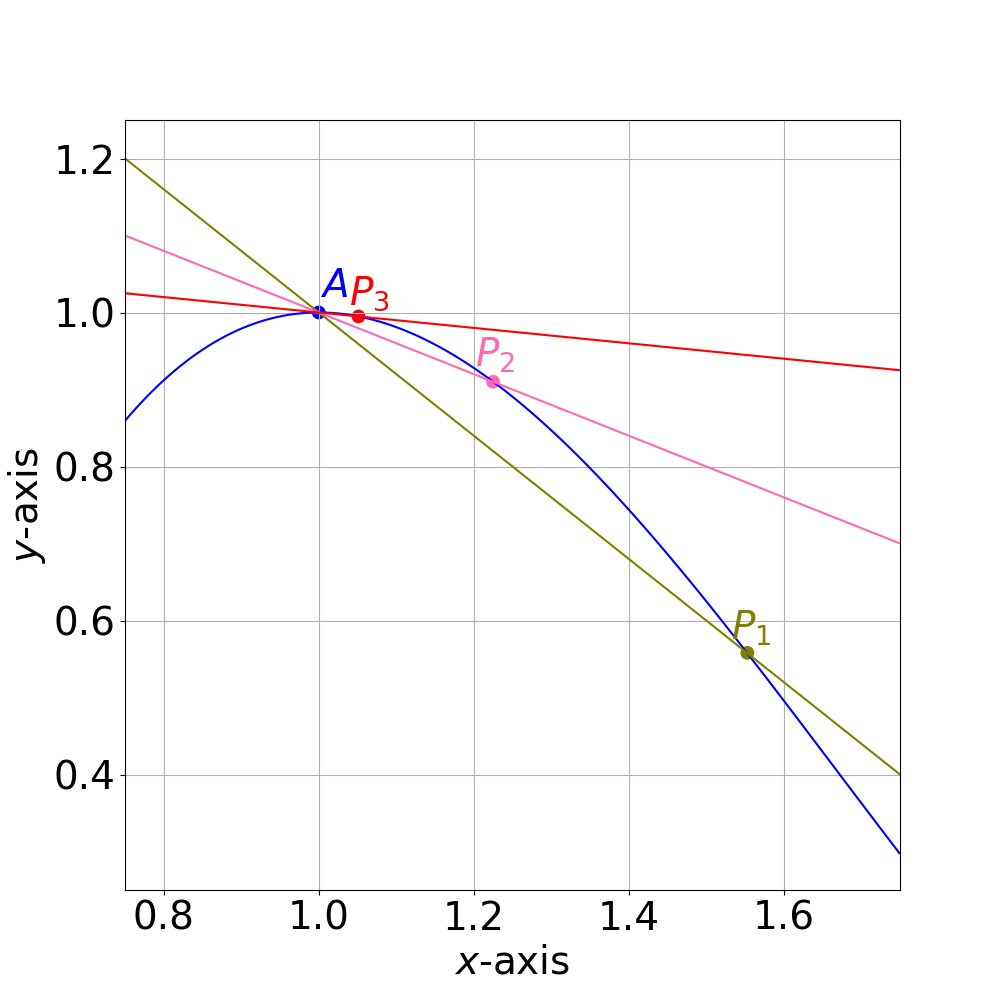
\includegraphics[width=0.6\textwidth]{sec_to_tan.png}\figtag{3.1.1}
\end{center}

As $h$ gets closer to $0$, the slope of each secant line indeed gets closer to the slope of the tangent line. If the limit of the slope of secants exists as $h$ approaches $0$, we just have the slope of the tangent line. For such kind of scenario, we say that the function is differentiable at $x$.

\begin{definition}[Differentiable and Derivative]
    A function $f$ is said to be \underline{differentiable} at $x$ if the limit $$\lim_{h\to 0}\dfrac{f(x+h)-f(x)}{h}$$ exists. If the limit exists, it is called the \underline{derivative} of $f$ at $x$ and is denoted by $f'(x)$. The symbol is read ``$f$ prime of $x$.''
\end{definition}

\begin{remark}
    We will say $f'(x)$ is ``the slope of $f$ at $x$'' for short-hand in the following context, instead of ``the slope of the tangent line of $f$ at $x$.''
\end{remark}

\begin{example}
    Find ${f_i}'(2)$, the slope of $f_i$ at $2$, if possible for the following functions.
    \begin{enumerate}
        \item $f_1(x)=x$.
        \item $f_2(x)=2x+5$.
        \item $f_3(x)=x^2$.
    \end{enumerate}
\end{example}
\textbf{Solution}. By definition, the slope of $f_i$ at $2$ is $${f_i}'(2)=\lim_{h\to 0}\dfrac{f_i(2+h)-f_i(2)}{h}.$$ Hence, \begin{align*}
    \lim_{h\to 0}\dfrac{f_1(2+h)-f_1(2)}{h}&=\lim_{h\to 0}\dfrac{2+h-2}{h}\\
    &=\lim_{h\to 0}1\\
    &=1,
\end{align*}
\begin{align*}
    \lim_{h\to 0}\dfrac{f_2(2+h)-f_2(2)}{h}&=\lim_{h\to 0}\dfrac{2(2+h)+5-(2\cdot2+5)}{h}\\
    &=\lim_{h\to 0}\dfrac{2h}{h}\\
    &=2,
\end{align*}
and \begin{align*}
    \lim_{h\to 0}\dfrac{f_3(2+h)-f_3(2)}{h}&=\lim_{h\to 0}\dfrac{(2+h)^2-(2)^2}{h}\\
    &=\lim_{h\to 0}\dfrac{4h+h^2}{h}\\
    &=\lim_{h\to 0}4+h\\
    &=4.
\end{align*} \qed

\begin{example}
    Let $t\in\bbR$. Find $f'(t)$, the slope of $f$ at $t$, if possible for $f(x)=x^2$.
\end{example}
\textbf{Solution}. By definition, the slope of $f$ at $t$ is \begin{align*}
    f'(t)&=\lim_{h\to 0}\dfrac{(t+h)^2-(t)^2}{h}\\
    &=\lim_{h\to 0}\dfrac{2th+h^2}{h}\\
    &=\lim_{h\to 0}2t+h\\
    &=2t.
\end{align*} \qed

In the previous example, $f'(t)=2t$ means that the function $f$ is going downwards at the left side of the $y$-axis and is going upwards at the right side of the $y$-axis.

In fact, the derivative $f'$ is also a function; it is only defined at points where $f$ is differentiable.

\begin{example}
    Let $t>0$. Find $f'(t)$, the slope of $f$ at $t$, if possible for $f(x)=\sqrt{x}$.
\end{example}
\textbf{Solution}. By definition, the slope of $f$ at $t$ is \begin{align*}
    f'(t)&=\lim_{h\to 0}\dfrac{\sqrt{t+h}-\sqrt{t}}{h}\\
    &=\lim_{h\to 0}\dfrac{\sqrt{t+h}-\sqrt{t}}{h}\cdot\dfrac{\sqrt{t+h}+\sqrt{t}}{\sqrt{t+h}+\sqrt{t}}\\
    &=\lim_{h\to 0}\dfrac{|t+h|-|t|}{h(\sqrt{t+h}+\sqrt{t})}\\
    &=\lim_{h\to 0}\dfrac{h}{h(\sqrt{t+h}+\sqrt{t})}\\
    &=\lim_{h\to 0}\dfrac{1}{\sqrt{t+h}+\sqrt{t}}\\
    &=\dfrac{1}{2\sqrt{t}}.
\end{align*} \qed

\begin{remark}
    In the previous example, $f'(0)$ does exist since the limit $$\lim_{h\to 0}\dfrac{\sqrt{0+h}-0}{h}=\lim_{h\to 0}\dfrac{1}{\sqrt{h}}$$ does not exist. Notice that the domain of $\sqrt{x}$ is $[0, \infty)$, but the domain of $\dfrac{1}{2\sqrt{t}}$ is $(0, \infty)$.
\end{remark}

\begin{example}
    Find the derivative $f'$ of $f(x)=\dfrac{1}{x}$ and state the domain of $f'$.
\end{example}
\textbf{Solution}. By definition, \begin{align*}
    \lim_{h\to 0}\dfrac{\dfrac{1}{x+h}-\dfrac{1}{x}}{h}&=\lim_{h\to 0}\dfrac{x-(x+h)}{h\cdot x\cdot(x+h)}\\
    &=\lim_{h\to 0}\dfrac{-h}{h\cdot x\cdot (x+h)}\\
    &=-\lim_{h\to 0}\dfrac{1}{x\cdot(x+h)}\\
    &=-\dfrac{1}{x^2}.
\end{align*} The domain of $f'(x)$ is $\bbR\setminus\{0\}$. \qed

\begin{example}
    Find the derivative $f'$ of $f(x)=e^x$.
\end{example}
\textbf{Solution}. By definition, \begin{align*}
    \lim_{h\to 0}\dfrac{e^{x+h}-e^x}{h}&=\lim_{h\to 0}\dfrac{e^x(e^h-1)}{h}\\
    &=e^x\lim_{h\to 0}\dfrac{e^h-1}{h}\\
    &=e^x\cdot 1\\
    &=e^x.
\end{align*} \qed

It turns out that the derivative of $e^x$ is itself. The action ``to find the derivative'' is called differentiate. That is, we differentiate a function $f$ to obtain its derivative (function) $f'$.

\begin{example}
    Differentiate $f(x)=\sin x$.
\end{example}
\textbf{Solution}. By definition, the derivative of $\sin x$ is \begin{align*}
    \lim_{h\to 0}\dfrac{\sin(x+h)-\sin x}{h}&=\lim_{h\to 0}\dfrac{\sin x\cos h+\cos x\sin h-\sin x}{h}\\
    &=\lim_{h\to 0}\dfrac{\sin x(\cos h-1)+\cos x\sin h}{h}\\
    &=\lim_{h\to 0}\dfrac{\sin x(\cos h-1)}{h}+\lim_{h\to 0}\dfrac{\cos x\sin h}{h}\\
    &=\sin x\cdot 0+\cos x\cdot 1\\
    &=\cos x.
\end{align*}
Hence, the derivative of $\sin x$ is $\cos x$. \qed

\begin{example}
    Find an equation of the tangent line to $f(x)=x^2$ at $3$.
\end{example}
\textbf{Solution}. Recall that a line $L$ with slope $m$ through point $(x_0, y_0)$ is $$L:y-y_0=m(x-x_0).$$ We know that the derivative of $x^2$ is $2x$; one should check it before proceed. Hence, the slope of $f$ at $3$ is $2\cdot 3=6$. Since $f(3)=9$, an equation for the tangent line to $f(x)=x^2$ at $3$ is $y-9=6(x-3)$. \qed

It strikes us that are continuous functions all differentiable? In fact, differentiable functions are continuous, but continuous functions are not deemed to be differentiable.

\begin{example}
    The absolute value function $f(x)=|x|$ is continuous on $\bbR$, but not differentiable at $0$.
\end{example}
\textbf{Proof}. It is clear that $f$ is differentiable on $\bbR\setminus\{0\}$. At $0$, \begin{align*}
    \lim_{h\to 0^+}\dfrac{|0+h|-|0|}{h}&=\lim_{h\to 0^+}\dfrac{h}{h}\\
    &=1,
\end{align*} but \begin{align*}
    \lim_{h\to 0^-}\dfrac{|0+h|-|0|}{h}&=\lim_{h\to 0^-}\dfrac{-h}{h}\\
    &=-1.
\end{align*} Since the two one-sided limits are not equal, the limit $\displaystyle\lim_{h\to 0}\dfrac{|0+h|-|0|}{h}$ does not exist. That is, $f$ is not differentiable at $0$. \qed

\begin{theorem}\label{diff->conti}
    If $f$ is differentiable at $c$, then $f$ is continuous at $c$.
\end{theorem}
\textbf{Proof}. Since $f$ is differentiable at $c$, the limit $$\lim_{h\to 0}\dfrac{f(c+h)-f(c)}{h}=f'(c).$$ Hence, \begin{align*}
    \lim_{h\to 0}f(c+h)-f(c)&=\lim_{h\to 0}\dfrac{f(c+h)-f(c)}{h}\cdot h\\
    &=\lim_{h\to 0}\dfrac{f(c+h)-f(c)}{h}\cdot \lim_{h\to 0} h\\
    &=f'(c)\cdot 0\\
    &=0.
\end{align*} \qed

\begin{remark}
    Through the contrapositive of Theorem \ref{diff->conti}, we know that if $f$ is not continuous at $c$, then $f$ is not differentiable at $c$.
\end{remark}

\subsection*{Exercise}

\begin{enumerate}[label=\arabic*.]
    \item Differentiate the following functions by definition.
    \begin{enumerate}
        \begin{multicols}{3}
            \item $f(x)=5-2x$.
            \item $f(x)=k, \quad k\in\bbR$.
            \item $f(x)=ax+b, \quad a, b\in\bbR$.
            \item $f(x)=x^3$.
            \item $f(x)=x^2-2x$.
            \item $f(x)=\dfrac{1}{\sqrt{x}}$.
            \item $f(x)=2x^3+c, \quad c\in\bbR$.
            \item $f(x)=\dfrac{8}{x+4}$.
            \item $f(x)=\sqrt{6-x}$.
        \end{multicols}
    \end{enumerate}
    \item Write an equation for the tangent line at $(c, f(c))$.
    \begin{enumerate}
        \begin{multicols}{2}
            \item $f(x)=x^2-2x, \quad c=1$.
            \item $f(x)=\dfrac{1}{x^2},\quad c=-1$.
            \item $f(x)=\sqrt{x-2}, \quad c=5$.
            \item $f(x)=2x^3-x^4, \quad c=-2$.
        \end{multicols}
    \end{enumerate}
    \item Find $f'(c)$ if it exists. Otherwise, explain the reason that the limit does not exist.
    \begin{enumerate}
        \begin{multicols}{2}
            \item $f(x)=\left\{\begin{array}{rl}
                6x, \quad & \text{if $x\leq 1$},\\
                3x^2+3, \quad & \text{if $x>1$},
            \end{array}\right.\quad c=1$.
            \item $f(x)=\left\{\begin{array}{rl}
                2x^2, \quad & \text{if $x\leq 0$},\\
                4x, \quad & \text{if $x>0$},
            \end{array}\right.\quad c=0$.
            \item $f(x)=\left\{\begin{array}{rl}
                x, \quad & \text{if $x<-1$},\\
                -\dfrac{1}{x}-2, \quad & \text{if $x\geq-1$},
            \end{array}\right.\quad c=-1$.
            \item $f(x)=\left\{\begin{array}{rl}
                x-2, \quad & \text{if $x\leq 2$},\\
                (x-2)^2, \quad & \text{if $x>2$},
            \end{array}\right.\quad c=2$.
            \item $f(x)=\left\{\begin{array}{rl}
                -\sqrt{-x}, \quad & \text{if $x<0$},\\
                \sqrt{x}, \quad & \text{if $x\geq 0$},
            \end{array}\right.\quad c=0$.
            \item $f(x)=\left\{\begin{array}{rl}
                -x^2, \quad & \text{if $x<0$},\\
                x^2, \quad & \text{if $x\geq 0$},
            \end{array}\right.\quad c=0$.
        \end{multicols}
    \end{enumerate}
    \item Differentiate $f(x)=\cos x$ by definition.
\end{enumerate}

\section{Differentiation Formulas}

Just like ones to continuous functions, there are operations tfor differentiable functions.

\setlength{\delimitershortfall}{0pt}
\begin{theorem}[Operations for Differentiable Functions]\label{diff_op}
    Let $\alpha\in\bbR$. If $f$ and $g$ are differentiable at $x$, then the following are true.
    \begin{enumerate}
        \item (\textit{Sum Rule}) The sum $f+g$ is differentiable, and the derivative of the sum is the sum of the derivatives, i.e., $(f+g)'=f'+g'$.
        \item (\textit{Scalar Multiple Rule}) The scalar product $\alpha f$ is differentiable, and the derivative of the scalar product is the scalar product of the derivative, i.e., $(\alpha f)'=\alpha f'$.
        \item (\textit{Product Rule}) The product $fg$ is differentiable, and $(fg)'=f'g+fg'$.
        \item (\textit{Reciprocal Rule}) If $g(x)\ne 0$, then the reciprocal of $g$ is differentiable, and $\left(\dfrac{1}{g}\right)'=-\dfrac{g'}{g^2}$.
    \end{enumerate}
\end{theorem}

\begin{example}
    Differentiate the following functions.
    \begin{enumerate}
        \item $f_1(x)=x^2$.
        \item $f_2(x)=x^n, \quad n\in\bbN$.
        \item $f_3(x)=x^{256}+x^{64}+x^{16}+4$.
        \item $f_4(x)=(4x^6+2x^3-7)(5x^2+x)$.
        \item $f_5(x)=\tan x$.
    \end{enumerate}
\end{example}
\textbf{Solution}. For $f_1$, we consider $x^2$ as $x\cdot x$ and use the product rule. That is, the derivative of $x^2$ is $1\cdot x+x\cdot 1=2x$. For $f_2$, we use induction on $n$ to show that the derivative of $x^n$ is $nx^{n-1}$. We already know the case $n=1$ holds. Suppose the derivative of $x^k$ is $kx^{k-1}$. Then, the derivative of $x^{k+1}$ is \begin{align*}
    1\cdot x^k+x\cdot kx^{k-1}&=x^k+kx^k\\
    &=(k+1)x^k.
\end{align*} We have hence proved the statement by induction. For $f_3$, we simply apply the sum rule with (ii) and have $${f_3}'(x)=256x^{255}+64x^{63}+16x^{15}.$$ For $f_4$, we use the product rule with (ii), having $${f_4}'(x)=(24x^5+6x)(5x^2+x)+(4x^6+2x^3-7)(10x).$$ For $f_5$, we use the product rule and the reciprocal rule together, having \begin{align*}
    {f_5}'(x)&=\cos x\cdot\dfrac{1}{\cos x}+\sin x\cdot\left(-\dfrac{-\sin x}{(\cos x)^2}\right)\\
    &=1+(\tan x)^2\\
    &=(\sec x)^2.
\end{align*} \qed
\setlength{\delimitershortfall}{13.5pt}

\begin{corollary}
    The derivative of $f(x)=x^k$ is $kx^{k-1}$ for all $k\in\mathbb{Z}\setminus\{0\}$.
\end{corollary}
\textbf{Proof}. The case for $k\in\bbN$ is already shown. For $k\in\mathbb{Z}$ with $k<0$, we simply apply the reciprocal rule, having \begin{align*}
    f'(x)&=-\dfrac{(-k)x^{-k-1}}{(x^{-k})^2}\\
    &=kx^{k-1}.
\end{align*} \qed

If one cannot see the first equation in the proof of the previous corollary, compare $$-\dfrac{(-k)x^{-k-1}}{(x^{-k})^2}\qquad\text{and}\qquad-\dfrac{g'}{g^2}.$$

\subsection*{Exercise}

\begin{enumerate}[label=\arabic*.]
    \item Differentiate the following functions.
    \begin{enumerate}
        \begin{multicols}{2}
            \item $f(x)=-x$.
            \item $f(x)=2-2x$.
            \item $f(x)=7x^3+2x^2+5$.
            \item $f(x)=\dfrac{e}{x^2}$.
            \item $f(x)=ax^2+bx+c, \quad a, b, c\in\bbR$.
            \item $f(x)=\dfrac{x^6}{6}+\dfrac{x^5}{5}+\dfrac{x^4}{4}+\dfrac{x^3}{3}+\dfrac{x^2}{2}+x+1$.
            \item $f(x)=\dfrac{1}{x^2+9}$.
            \item $f(x)=\dfrac{x^2+9}{x}$.
            \item $f(x)=\dfrac{x^4-4}{x^2-2}$.
            \item $f(x)=\dfrac{1+x^3}{2x^2-1}$.
            \item $f(x)=(5x^4-7x^2+1)\cdot(x^{12}+4x^5+3x-2)$.
            \item $f(x)=\dfrac{x^2-1}{x^2+1}$.
        \end{multicols}
    \end{enumerate}
    \item Find an equation for the tangent line at the point $(c, f(c))$.
    \begin{enumerate}
        \begin{multicols}{2}
            \item $f(x)=x^3+3x+6, c=-1$.
            \item $f(x)=\dfrac{5}{x^2+1}, c=2$.
        \end{multicols}
    \end{enumerate}
    \item Differentiate the following functions.
    \begin{enumerate}
        \begin{multicols}{3}
            \item $f(x)=\cot x$.
            \item $f(x)=\sec x$.
            \item $f(x)=\csc x$.
        \end{multicols}
    \end{enumerate}
    \item Find the number pair $(A, B)$ such that the derivative of $f$ is everywhere continuous for the following functions.
    \begin{enumerate}
        \begin{multicols}{2}
            \item $f(x)=\left\{\begin{array}{rl}
                Ax^3+Bx+2, \quad &\text{if $x\leq 2$},\\
                Bx^2-A, &\text{if $x>2$}.
            \end{array}\right.$
            \item $f(x)=\left\{\begin{array}{rl}
                Ax^2+B, \quad &\text{if $x<-1$},\\
                Bx^5+Ax+4, &\text{if $x\geq -1$}.
            \end{array}\right.$
        \end{multicols}
    \end{enumerate}
\end{enumerate}

\section{Derivatives of Higher Orders}

\section{The Chain Rule}

% Graph drawing, l'Hospital
\chapter{Application of Differentiation}



% Formulae for antiderivatives
\chapter{Integral and Integration}



% sub, IBP
\chapter{Techniques of Integration}



\chapter{Numerical Sequences, Numerical Series, and Power Series}



\chapter{Multivariable Differentiation}



\chapter{Multiple Integrals}


\end{document}